\documentclass[master,openany]{tongjithesis}
% \documentclass[%
%   master|doctor, % mandatory option
%   xetex|pdftex|dvips|dvipdfm, % optional
%   utf|gbk,
%   electronic,
%   openany|openright]{tongjithesis}

% 所有其它可能用到的包都统一放到这里了,可以根据自己的实际添加或者删除。
\usepackage{tongjiutils}
\usepackage[top=3.23cm, bottom=2.54cm, left=3.17cm, right=3.17cm]{geometry}

% 显示交叉引用的标签
%\usepackage{showkeys}

% 显示页面布局
%\usepackage{layout}

\def\myname{李勇奇}

\begin{document}

% 显示页面布局
%\layout

\graphicspath{{fig/}}

%%% 封面部分
\frontmatter
%!TEX root = ../thesis.tex

% 保密文字位置可能有问题,需要到cls文件中调整
\secretlevel{保密} \secretyear{2}

\ctitle{基于RGB-D图像的三维物体识别算法的研究与实现}
% 按照申请工学学位设计。如有其它需要,请修改相应文字。
\makeatletter
  \iftongji@doctor
    \cdegree{博士}
  \else
    \iftongji@master
      \cdegree{硕士}
    \fi
  \fi

\makeatother

\cauthor{李勇奇} % 姓名

\snumber{1531620}  % 学号

\cdepartment{电子与信息工程学院}

\cmajorfirst{工学}

\cmajorsecond{控制科学与工程}

\csupervisor{陈启军 ~ 教授}

\cassosupervisor{}
% 如果没有副指导老师或者联合指导老师,把各自{}中内容留空即可。

\ccosupervisor{}

% 日期自动生成,如果你要自己写就改这个cdate
%\cdate{\CJKdigits{\the\year}年\CJKnumber{\the\month}月}
\makeatletter
  \iftongji@doctor
    \edegree{Doctor of Philosophy}
  \else
    \iftongji@master
      \edegree{Master of Engineering}
    \fi
  \fi

\makeatother

%\cfunds{国家自然科学基金资助(项目号:XXXXXX)}

%\efunds{Supported by the Natural Science Foundation of China(No.XXXXXX)}


\etitle{3D Object Recognition and Pose Estimation \\ Based on RGB-D Images}

\eauthor{Li Yongqi}

\edepartment{College of Electronics and Information Engineering}

\emajorfirst{Engineering}%Science in

\emajorsecond{Control Science and Engineering}

\esupervisor{Prof. ~ Chen Qijun}
\eassosupervisor{}

% 这个日期也会自动生成,你要改么?
%\edate{March, 2017}

% 定义中英文摘要和关键字
\begin{cabstract}
  三维视觉是机器人感知的重要组成部分,但其目前的技术水平难以帮助机器人有效地感知周围的三维世界。随着近几年深度学习的发展,计算机视觉领域取得了巨大的发展,尤其是在2D视觉领域,2D目标的检测和分类的准确率得到了巨大的提升,但3D目标的检测并没有巨大的提升。因此,本文针对机器人目前三维感知的困难,通过参考深度学习在2D视觉上的突破,将其引入到3D视觉上来,提出了3D-MRAI算法,用于解决对3D目标的检测以及位姿的估计。

  深度信息的质量对3D目标检测以及位姿估计的准确率和精度都有至关重要的影响,因此为了获取高质量的深度信息,本文针对现有RGB-D相机的缺点,提出了对偶RGB-D相机结构,通过组合两个低价的RGB-D相机来获取高质量的深度信息,提高了相机获取深度图的填充率并且增强了深度信息的鲁棒性。

  为了能够在RGB-D图中检测出目标物体的种类以及位姿,本文提出的3D-MRAI算法分为两步,第一步在相机拍摄的三维点云中分割出目标物体点云;第二步通过点云匹配算法求解出目标的位姿。为了分割出目标物体点云,本文基于2D目标检测中的Faster R-CNN和Mask R-CNN两个算法,提出了3D Faster R-CNN和3D Mask R-CNN算法,3D Faster R-CNN和3D Mask R-CNN通过将深度图变换为HHA图,有效地利用三维信息,并结合RGB图完成对目标物体的检测,并且为了应对目标物体的各种姿态,算法还引入了Spatial Transformer结构。3D Faster R-CNN和3D Mask R-CNN相比Faster R-CNN和Mask R-CNN充分利用三维信息,对检测一些纹理较少(Textureless)的物体有着更高的准确率。为了求解目标的位姿,本文通过匹配目标物体点云和目标物体3D模型来实现,为此基于4PCS算法提出了A4PCS-ICP点云匹配算法,通过在改进4PCS算法的基础上引入ICP算法提高了匹配精度。

  本文还将所提出的3D-MRAI算法实际应用到Bin-Picking问题上,设计了一个基于3D-MARI算法的随机分拣视觉系统,所设计的系统在实验中达到了100\%的抓取成功率,并且算法的运算时间也完全满足实际应用。
\end{cabstract}

\ckeywords{RGB-D,目标检测,位姿估计,随机分拣}


\begin{eabstract}
3D vision is an important part of robot perception, but the technology of 3D vision currently is hard to help robots effectively perceive the surrounding 3D world. With the development of deep learning in recent years, tremendous development has been made in the field of computer vision. Especially in the field of 2D vision, the accuracy of 2D object detection and classification has been greatly improved, but the detection of 3D objects has not been huge Enhance. Therefore, for the difficulty of current 3D robot perception. This paper proposed a new algorithm 3D-MRAI, which introduced deep learning into 3D vision based on the breakthrough of deep learning in 2D vision. This algorithm is proposed to solve the problem of 3D object detection and pose estimation .

High-quality depth map has a great influence on the results of 3D object detection and pose estimation. To acquire high-quality depth map, a dual RGB-D camera structure is proposed to overcome the shortcomings of the existing RGB-D cameras. Dual RGB-D camera can obtain high-quality depth map by combining two low-cost RGB-D cameras, which also increases the fill rate of depth map and enhances depth value in depth map.

To detect object and estimate pose in a given RGB-D frame, 3D-MRAI algorithm proposed this paper runs in two stage. The first stage is to get the point cloud of the object from the RGB-D frame. The second stage is to estimate the object pose by point cloud matching. To segement the point cloud of the object, 3D Faster R-CNN and 3D Mask R-CNN are proposed based on two algorithm in 2D object detection: Faster R-CNN and Mask R-CNN. 3D Faster R-CNN and 3D Mask R-CNN take full advantage of depth value by converting depth map into HHA frame and detect object by combining RGB and HHA. 3D Faster R-CNN and 3D Mask R-CNN also use Spatial Transformer to detect object in arbitrary pose.  3D Faster R-CNN and 3D Mask R-CNN have higher detection accuracy when detecting textureless objects, comparing to Faster R-CNN and Mask R-CNN. In order to estimate the pose of the target, we match the 3D model of the object to the point cloud of the object. For this purpose, a new point cloud matching algorithm call A4PCS-ICP is proposed. A4PCS-ICP algorithm has higher matching accuracy by combining ICP and modified 4PCS.

  This paper also applies the proposed 3D-MRAI algorithm to solve the Bin-Picking problem. A bin-picking vision system is designed based on 3D-MARI algorithm. The designed system achieves 100\% successful picking rate, and the system's response time also fully meets the application.

\end{eabstract}

\ekeywords{RGB-D, object detection, pose estimation, Bin-Picking}

%%% Local Variables:
%%% TeX-master: "../thesis.tex"
%%% End:
\makecover

% 目录
\tableofcontents

% 符号对照表
% %!TEX root = ../thesis.tex
\begin{denotation}
\item[GNU] GNU's Not Unix /'gnu:/
\item[GFDL] GNU Free Documentation License
\item[GPL] GNU General Public License
\item[FSF] Free Software Foundation
\end{denotation}


%%% 以下索引按需要选择
% 插图索引
%\listoffigures
% 表格索引
%\listoftables
% 公式索引
%\listofequations

%%% 正文
\mainmatter
\chapter{引言}
\label{chap:introduction}
本文\cite{tex}

%%% Local Variables:
%%% TeX-master: "../thesis.tex"
%%% End:
%!TEX root = ../thesis.tex
\chapter{RGB-D图像的获取与融合}
\label{chap:rgbd}

\section{3D相机现状与分析}
% @TODO: 3d相机现状

\section{RGB-D相机}
\subsection{RGB-D相机原理与结构}
RGB-D相机获取深度的原理大致可以分为三种:
\begin{itemize}
\item Structure Light
\item Time of Flight(ToF)
\item Stereo
\end{itemize}

% @TODO: 加些原理图?
Structure Light获取深度信息的原理是通过激光发射器投射带有特定编码的结构光到物体表面后,由IR Camera采集,根据采集到的光信号量的变化来计算物体的深度。举一个形象的例子,将手电筒照向墙面,手电筒离墙面越远,墙面上所形成的光斑的直径就越大,所以可以通过光斑的直径来计算手电筒距离墙面的距离。ToF获取深度信息的原理是通过专有的传感器捕捉红外光发射到接收的飞行时间来计算物体的深度。Stereo是通过双摄像头拍摄物体,再通过特征点匹配,根据三角测量原理来计算物体的深度。

三种原理的深度相机各有其特点,采用Structure Light原理的深度相机一般精度比较高,但景深比较短并且受光线影响比较大,适合室内场景;ToF原理的深度相机获取深度图的精度和分辨率一般都比较低,但帧率高,并且具有一定的抗光照性能;Stereo获取深度精度适中,帧率相对来说较低,并且需要较强的计算性能,但抗光照能力强,适合室外场景。

本文所使用的RGB-D相机是Intel的Realsense SR300相机,SR300采用的结构光的原理获取深度\footnote{此后所提到的RGB-D相机均指与SR300相机类似的采用结构光原理获取深度的RGB-D相机},其内部结构如图\ref{fig:sr300}所示。
\begin{figure}[!ht]
  \centering
  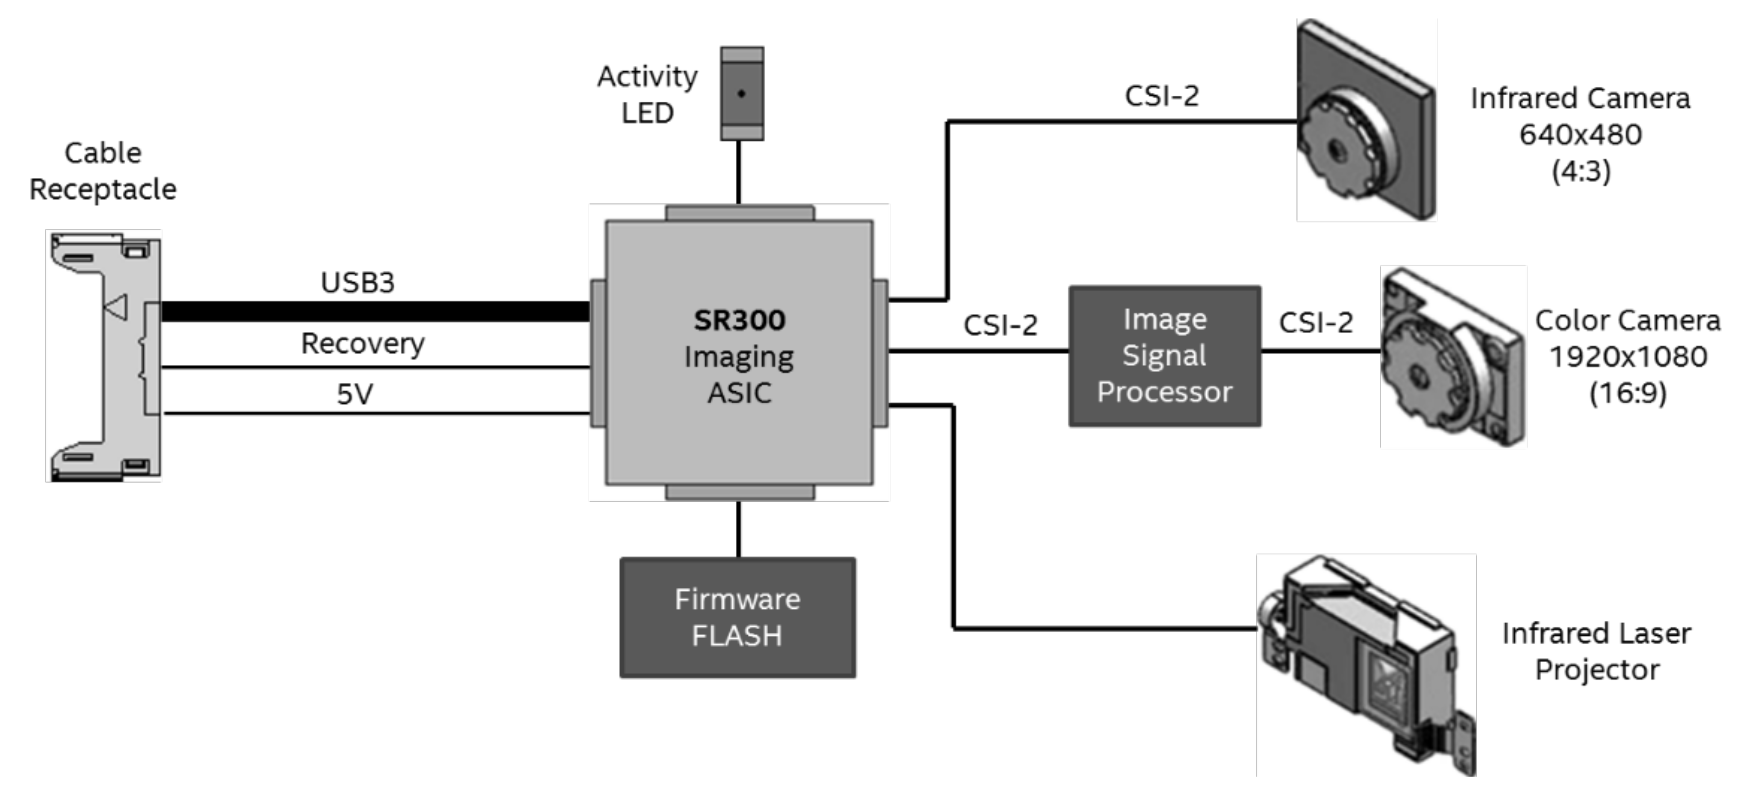
\includegraphics[width=12cm]{sr300}
  \caption{Realsense SR300内部结构图}
  \label{fig:sr300}
\end{figure}
从图\ref{fig:sr300}可以看出,SR300内部的传感器主要有彩色摄像头(Color Camera)、红外激光发射器(Infrared Laser Projector)和红外摄像头(Infrared Camera)。Color Camera是1920×1080像素的普通针孔摄像头,用来获取彩色图像;Infrared Laser Projector和Infrared Camera用来获取深度图像或者红外成像图,两种成像流程如图\ref{fig:capture_flow}所示。
\begin{figure}[!ht]
  \centering
  \subfloat[Depth Video Data Flow]{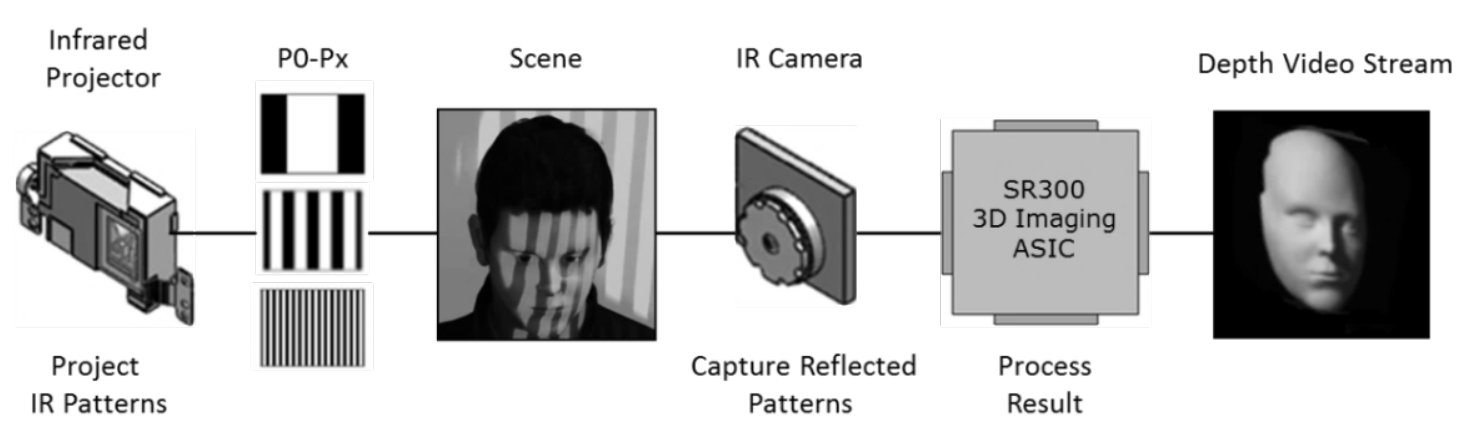
\includegraphics[width=12cm]{depth_flow}}
  \vfill
  \subfloat[IR Video Data Flow]{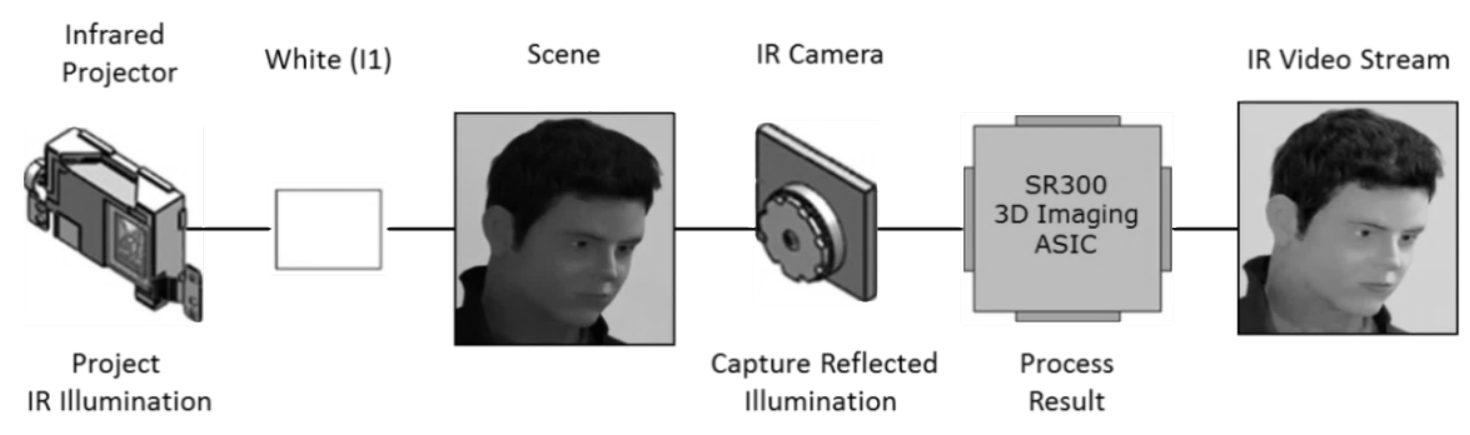
\includegraphics[width=12cm]{ir_flow}}
  \caption{Realsense SR300深度成像流程}
  \label{fig:capture_flow}
\end{figure}
其中当Infrared Laser Projector投射带有编码的结构光时,Infrared Camera可以获取深度图;当投射不带编码的红外光时,Infrared Camera可以获取红外成像图。正常使用时,往往设置Infrared Laser Projector投射带有编码的结构光来获取深度信息。因此,从RGB-D相机的使用来看,可以忽略其内部具体结构,将其看成由一个彩色摄像头和一个深度摄像头构成,其中彩色摄像获取彩色(RGB)信息,深度摄像头获取深度(depth)信息。

\subsection{RGB-D相机的数学模型}
\begin{figure}[!ht]
  \centering
  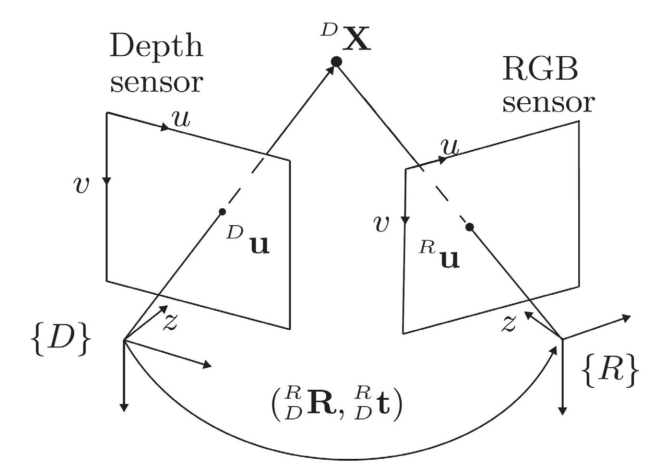
\includegraphics[width=8cm]{rgbd_model}
  \caption{RGB-D相机模型}
  \label{fig:rgbd_model}
\end{figure}
图\ref{fig:rgbd_model}展示了本文所使用的RGB-D相机的基本物理模型,其中彩色摄像头和深度摄像头都使用了针孔(pin-hole)相机模型\cite{Heikkila2000}。
先考虑普通针孔相机的模型,相机图像坐标系下一点$\bm{u}:=[u,v]^T$,对应的三维世界中的一点在相机坐标系下表示为$\bm{X}:=[x,y,z]^T$。根据针孔相机模型有:
\begin{equation}
  \label{eq:cam_model}
  z\bm{\tilde{u}} = \bm{K}\bm{X}
\end{equation}
其中$\bm{\tilde{u}}$表示$\bm{u}$的齐次变换形式,彩色相机的内参矩阵$\bm{K}$的定义如下:
\begin{equation}
  \bm{K} := \left[
    \begin{array}{ccc}
      f_u&0&u_0 \\
      0&f_v&v_0 \\
      0&0&1
    \end{array}
  \right]
\end{equation}
其中$f_u$和$f_v$分别表示彩色相机在图像坐标轴上的焦距(以像素为单位),$u_0$和$v_0$表示彩色相机光心在图像平面的投影中心。

公式\ref{eq:cam_model}还未考虑镜头的畸变,为了提高相机的精度,现引入径向畸变(radial distortion)和切向畸变(tangential distortion):
\begin{itemize}
\item 径向畸变是由相机透镜的不完善和表面曲率存在误差造成的,径向畸变的数学模型可以表示为:
  \begin{equation}
    \label{eq:radial}
    \left\{
      \begin{array}{ccc}
        \hat{x}&=&\bar{x}(1 + k_1r^2 + k_2r^4 + k_3r^6)\\
        \hat{y}&=&\bar{y}(1 + k_1r^2 + k_2r^4 + k_3r^6)\\
      \end{array}
    \right.
  \end{equation}
  其中
  \begin{align}
    \bar{x} =& x/z\\
    \bar{y} =& y/z\\
    r  =& \sqrt{\bar{x}^2 + \bar{y}^2}
  \end{align}
  $\bar{x}$,$\bar{y}$表示点$\bm{X}$在归一化平面上的坐标,$\hat{x}$,$\hat{y}$表示修正径向畸变后的的坐标,$k_1$,$k_2$,$k_3$表示径向畸变的参数。
\item 切向畸变是由于相机透镜与图像平面不平行造成的,其数字模型可以表示为:
  \begin{equation}
    \label{eq:trang}
    \left\{
      \begin{array}{ccc}
        \hat{x}&=&\bar{x} + (2p_1\bar{x}\bar{y} + p_2(r^2 + 2\bar{x}^2))\\
        \hat{y}&=&\bar{y} + (p_1(r^2 + 2\bar{y}^2) + 2p_2\bar{x}\bar{y})\\
      \end{array}
    \right.
  \end{equation}
  其中$p_1$,$p_2$是切向畸变的参数。
\item 结合公式\ref{eq:radial}和\ref{eq:trang}可以得到修正径向畸变和切向畸变的Brown–Conrady模型\cite{Brown1966}:
  \begin{equation}
    \label{eq:dist}
    \left\{
      \begin{array}{ccc}
        \hat{x}&=&\bar{x}(1 + k_1r^2 + k_2r^4 + k_3r^6) + (2p_1\bar{x}\bar{y} + p_2(r^2 + 2\bar{x}^2))\\
        \hat{y}&=&\bar{y}(1 + k_1r^2 + k_2r^4 + k_3r^6) + (p_1(r^2 + 2\bar{y}^2) + 2p_2\bar{x}\bar{y})\\
      \end{array}
    \right.
  \end{equation}
\end{itemize}
通过以上分析,根据公式\ref{eq:cam_model}和\ref{eq:dist}可以推导出带有畸变的针孔相机模型:
\begin{equation}
  \label{eq:dist_cam_model}
  \left\{
    \begin{array}{ccc}
      u&=&f_u(\bar{x}(1 + k_1r^2 + k_2r^4 + k_3r^6) + (2p_1\bar{x}\bar{y} + p_2(r^2 + 2\bar{x}^2))) + u_0\\
      v&=&f_v(\bar{y}(1 + k_1r^2 + k_2r^4 + k_3r^6) + (p_1(r^2 + 2\bar{y}^2) + 2p_2\bar{x}\bar{y})) + v_0
    \end{array}
  \right.
\end{equation}
为方便起见,记$\bm{d}:=[k_1,k_2,p_1,p_2,k_3]^T$,定义函数
\begin{equation}
  f_{undist}(\bm{d}, \bm{X}):=\left[
    \begin{array}{ccc}
      \bar{x}(1 + k_1r^2 + k_2r^4 + k_3r^6) + (2p_1\bar{x}\bar{y} + p_2(r^2 + 2\bar{x}^2))\\
      \bar{y}(1 + k_1r^2 + k_2r^4 + k_3r^6) + (p_1(r^2 + 2\bar{y}^2) + 2p_2\bar{x}\bar{y})\\
    \end{array}
  \right]
\end{equation}
\begin{equation}
  \tilde{f}_{undist}(\bm{d}, \bm{X}):=\left[
    \begin{array}{c}
      f_{undist}(\bm{d}, \bm{X})\\
      1
    \end{array}
  \right]
\end{equation}
则公式\ref{eq:dist_cam_model}可简化为:
\begin{equation}
  \tilde{\bm{u}} = \bm{K}\cdot \tilde{f}_{undist}(\bm{d}, \bm{X})
\end{equation}
其中需要标定的参数有相机内参矩阵$\bm{K}$(包含未知参数$f_u$,$f_v$,$u_0$,$v_0$)以及畸变参数$\bm{d}$(包含未知参数$k_1$,$k_2$,$p_1$,$p_2$,$k_3$),共9个参数。

明确了针孔相机的数学模型后,很容易推出SR300的相机模型:
\begin{equation}
  \label{eq:rgbd_cam_model}
  \left\{
    \begin{array}{ccc}
      \tensor*[^R]{\tilde{\bm{u}}}{}&=&\tensor*[^R]{\bm{K}}{}\cdot \tilde{f}_{undist}(\tensor*[^R]{\bm{d}}{},\tensor*[^R]{\bm{X}}{})\\
      \tensor*[^D]{\tilde{\bm{u}}}{}&=&\tensor*[^D]{\bm{K}}{}\cdot \tilde{f}_{undist}(\tensor*[^D]{\bm{d}}{},\tensor*[^D]{\bm{X}}{})\\
      \tensor*[^R]{\bm{X}}{} &=& \tensor*[^R_D]{\,\bm{R}}{}\tensor*[^D]{\bm{X}}{} + \tensor*[^R_D]{\,\bm{t}}{}
    \end{array}
  \right.
\end{equation}
其中左上标$\{R\}$表示SR300相机中的彩色相机(RGB),$\{D\}$表示SR300相机中的深度相机(Depth),$\tensor*[^R_D]{\,\bm{R}}{}$和$\tensor*[^R_D]{\,\bm{t}}{}$表示了彩色相机坐标系和深度相机坐标系之间的齐次变换关系。

\subsection{RGB-D相机的标定流程}
\label{sec:rgb-d_calibration}
根据上文所述的RGB-D相机的结构及数学模型,RGB-D相机的标定主要涉及到彩色摄像头内参和畸变的标定,深度摄像头内参和畸变的标定,以及彩色摄像头和深度摄像头之间位姿变换的标定。由于RGB-D相机是一种较为新颖的相机,所以市面上基本上没有较为成熟通用的标定RGB-D相机的方法以及对应的工具。因此本文针对所使用的Realsense SR300相机,设计了一套标定方法。

根据公式\ref{eq:rgbd_cam_model}可知相机需要标定的参数有彩色相机内参和畸变参数9个,深度相机内参和畸变参数9个,彩色相机和深度相机之间的位姿关系6个,一共24个参数。一起标定这24个参数理论上是相当困难的,考虑到普通针孔相机的标定技术已经相当成熟(如张正友的棋盘格标定\cite{Zhang2002},以及RGB-D相机中彩色相机和深度相机的解耦性,因此所设计的标定方法分为三步:
\begin{enumerate}[Step 1]
\item 标定彩色相机内参以及畸变参数
\item 标定深度相机内参以及畸变参数
\item 标定彩色相机和深度相机之间的齐次变换关系
\end{enumerate}

步骤1标定彩色相机内参以及畸变参数相对来说比较简单,主要参考文献\cite{Zhang2002},但所使用的标定板是不对称圆盘标定板(Asymmetrical Circle Board),如图\ref{fig:circle_board}是$4\times 11$的不对称圆盘标定板。
\begin{figure}[!ht]
  \centering
  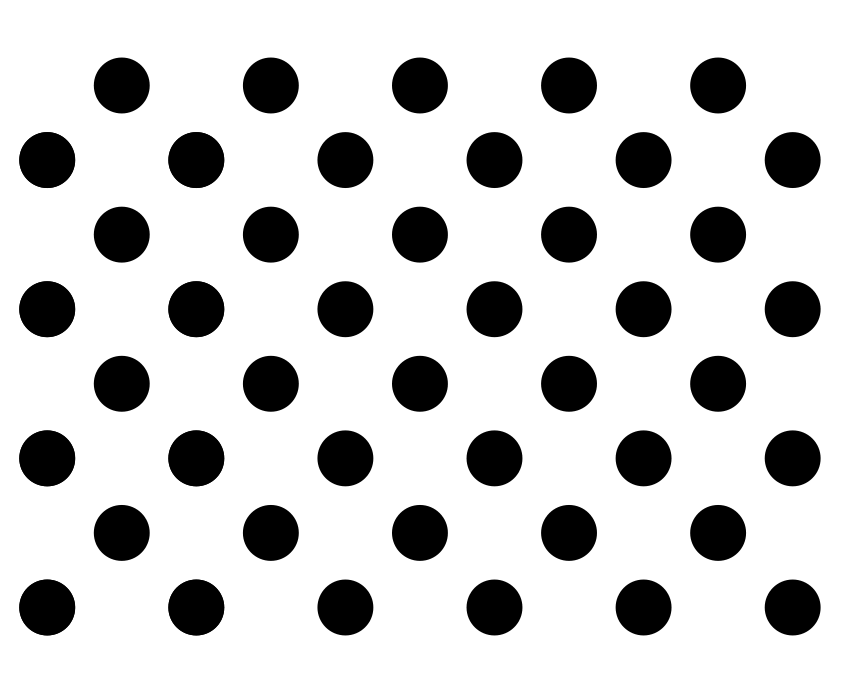
\includegraphics[width=10cm]{circle_board}
  \caption{Asymmetrical Circle Board}
  \label{fig:circle_board}
\end{figure}
使用圆盘标定板而非棋盘格标定板的原因是圆盘相对于棋盘格有更高的检测精度,在某些情况下可以达到0.1到0.01像素的亚像素精度,当然代价是相比计算棋盘格的角点,计算椭圆(圆形经过投影变换后退化为椭圆)的中心会涉及到较为复杂的数学运算,这也是为什么工业上大多使用圆盘作为标定板的原因。

步骤2标定深度相机内参以及畸变参数的方法和步骤1类似,区别在于深度相机并不能直接获得颜色信息,因此也不能直接检测图\ref{fig:circle_board}所示的标定板。但是,幸运的是,根据前文所述的SR300深度相机的原理,其本质上也是个普通的针孔相机,只不过在其镜头上加上了滤波片,可以认为其只对红外光成像。因此,只要使用图\ref{fig:capture_flow}中的红外成像模式获取红外成像图,在红外成像图上检测标定板。如图\ref{fig:circle_on_ir}所示,在红外成像图中检测出了标定板。
\begin{figure}[!ht]
  \centering
  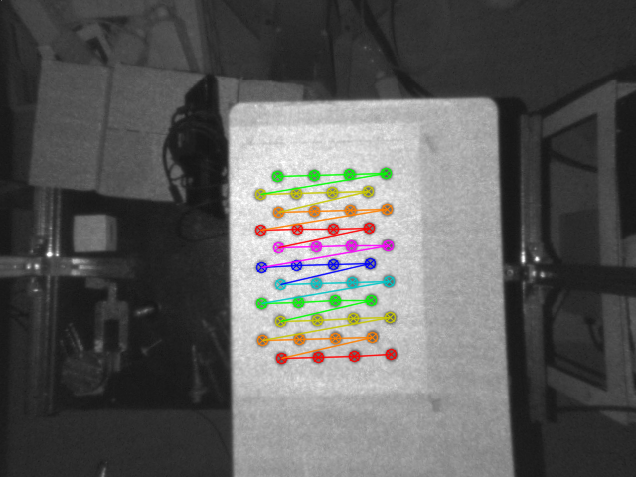
\includegraphics[width=12cm]{circle_on_ir}
  \caption{红外成像图中检测标定板}
  \label{fig:circle_on_ir}
\end{figure}

步骤3标定彩色相机和深度相机之间的齐次变换关系需要依赖于步骤1和步骤2中标定出的彩色相机和深度相机的内参和畸变参数,具体做法是将标定板放在彩色相机和深度相机下,使彩色相机和深度相机能够同时检测到标定板,然后分别根据各自的内参和畸变参数计算出标定板的位姿$\tensor*[^R_B]{\bm{H}}{}$和$\tensor*[^D_B]{\bm{H}}{}$,其中$\tensor*[^R_B]{\bm{H}}{}$是$4\times 4$的齐次变换矩阵,表示标定板在彩色相机坐标系下的位姿,也是彩色相机坐标系变换到标定板坐标系的齐次变换矩阵;$\tensor*[^D_B]{\bm{H}}{}$也是$4\times 4$的齐次变换矩阵,表示标定板在深度相机坐标系下的位姿,也是深度相机坐标系变换到标定板坐标系的齐次变换矩阵。从而所要求的彩色相机坐标系变换到深度相机坐标系的齐次变换矩阵为:
\begin{equation}
  \tensor*[^R_D]{\bm{H}}{} = \tensor*[^R_B]{\bm{H}}{}\tensor*[^D_B]{\bm{H}}{^{-1}}
\end{equation}
其中
\begin{equation}
  \tensor*[^R_D]{\bm{H}}{} := \left[
    \begin{array}{cc}
      \tensor*[^R_D]{\bm{R}}{}& \tensor*[^R_D]{\bm{t}}{}\\
      \bm{0}_{1\times 3}&1
    \end{array}
\right]
\end{equation}
当然,实际标定时,往往会采取多组$\tensor*[^R_B]{\bm{H}}{}$和$\tensor*[^D_B]{\bm{H}}{}$来提高标定的精度。

\section{对偶RGB-D相机}
使用SR300相机时,发现相机在某些情况下,对一些反光的物体的深度图有严重的缺失,具体如图\ref{fig:depth_missing}所示。
\begin{figure}[!ht]
  \centering
  \subfloat[彩色图]{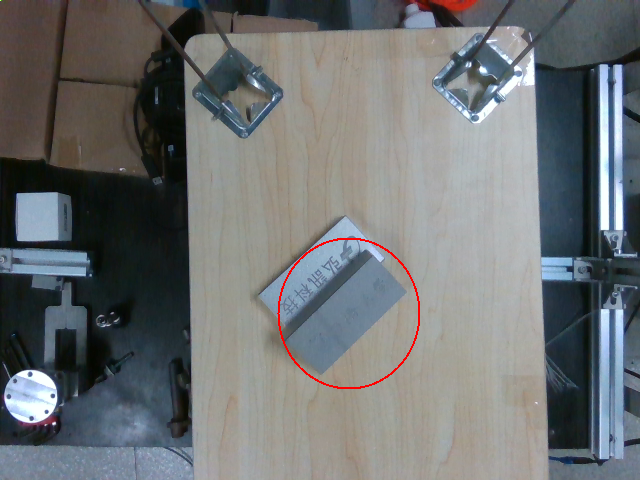
\includegraphics[width=7cm]{left_color}}
  \hfill
  \subfloat[深度图]{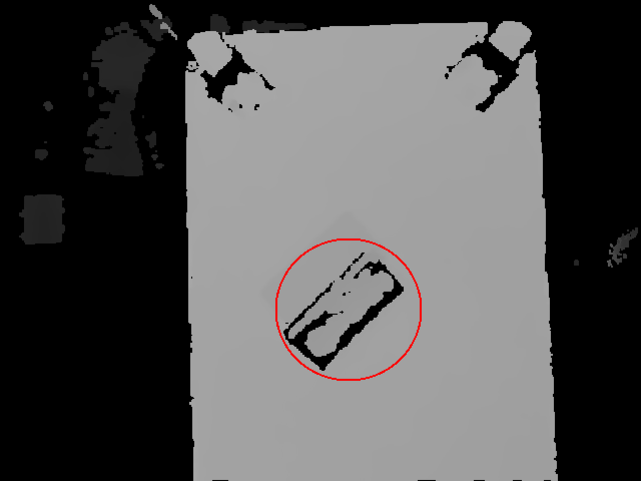
\includegraphics[width=7cm]{left_depth}}
  \caption{SR300采集的物体深度信息部分缺失情况下的深度图}
  \label{fig:depth_missing}
\end{figure}
经过实验,发现这种缺失情况的出现和拍摄的角度以及光线有关,因此本文提出一种组合相机对偶RGB-D相机(Dual RGB-D Camera)。

\subsection{对偶RGB-D相机原理与结构}
对偶RGB-D相机在原RGB-D相机的基础上,通过增加一个与原相机呈180度夹角的RGB-D相机构成,实际物理结构如图\ref{fig:dual_rgbd}所示。
\begin{figure}[!ht]
  \centering
  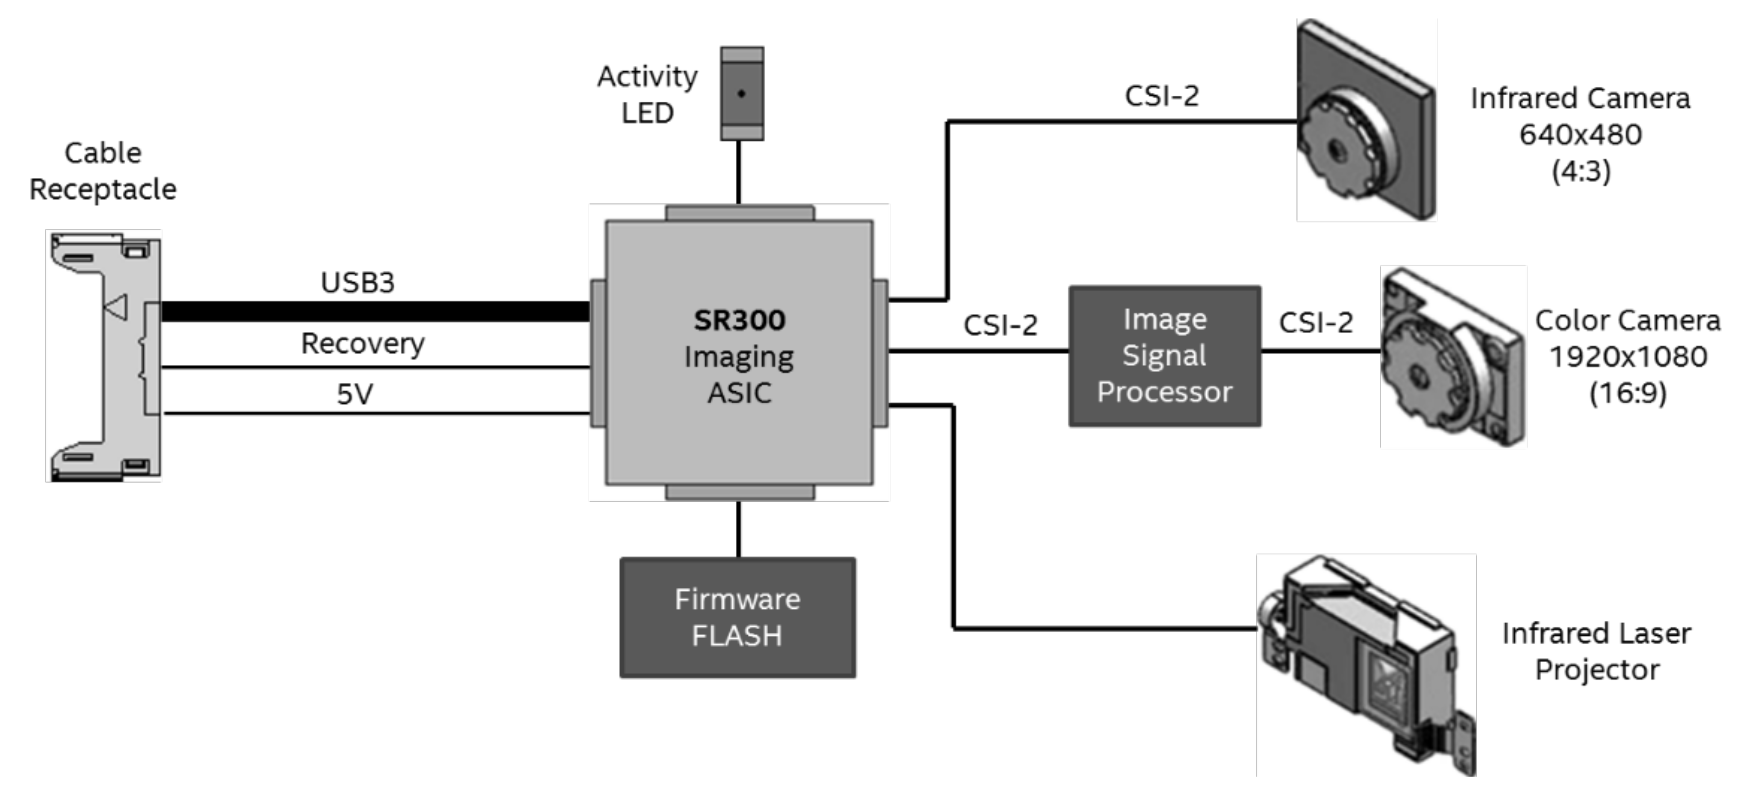
\includegraphics[width=6cm]{dual_rgbd}
  \caption{对偶RGB-D相机实际物理结构}
  \label{fig:dual_rgbd}
\end{figure}

对于对偶RGB-D相机,当其中一个相机深度图出现严重缺失时,另外一个相机的深度图往往不会在相同的地方深度信息出现严重的缺失,如图\ref{fig:dual_rgbd_depth}所示\footnote{实际下相机采集的图像与上相机采集的图像相差了180度,为了方便起见,都将下相机采集的图像旋转了180度}
,有效的避免了单个RGB-D相机某些情况下深度信息严重缺失的情况。
\begin{figure}[!ht]
  \centering
  \subfloat[上相机采集的深度图]{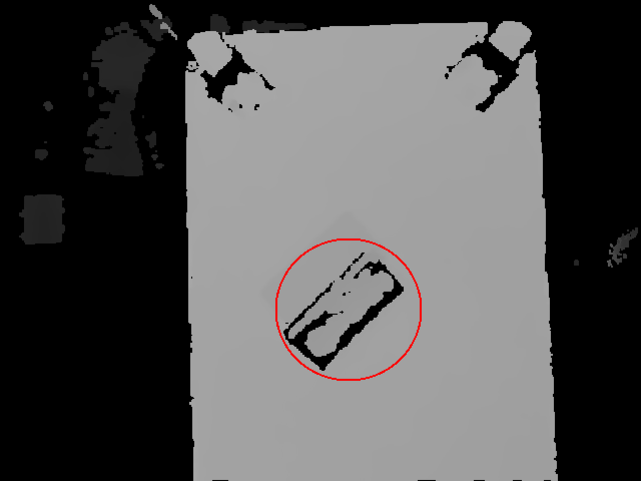
\includegraphics[width=7cm]{left_depth}}
  \hfill
  \subfloat[下相机采集的深度图]{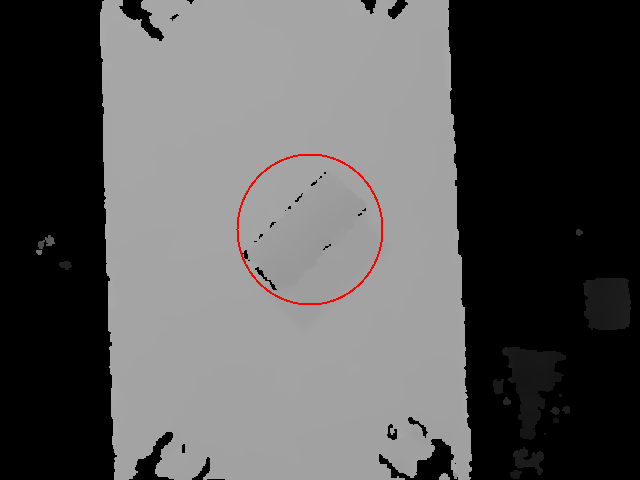
\includegraphics[width=7cm, angle=180, origin=c]{right_depth}}
  \caption{对偶RGB-D相机采集的左右两张深度图}
  \label{fig:dual_rgbd_depth}
\end{figure}

除此之外,对偶RGB-D相机还可以利用两个相机的彩色图构成双目,生成第三张深度图,从而通过设计的深度的融合算法将三张深度图融合成为一张质量更高的深度图,其内部原理如图\ref{fig:dual_rgbd_struct}所示。
\begin{figure}[!ht]
  \centering
  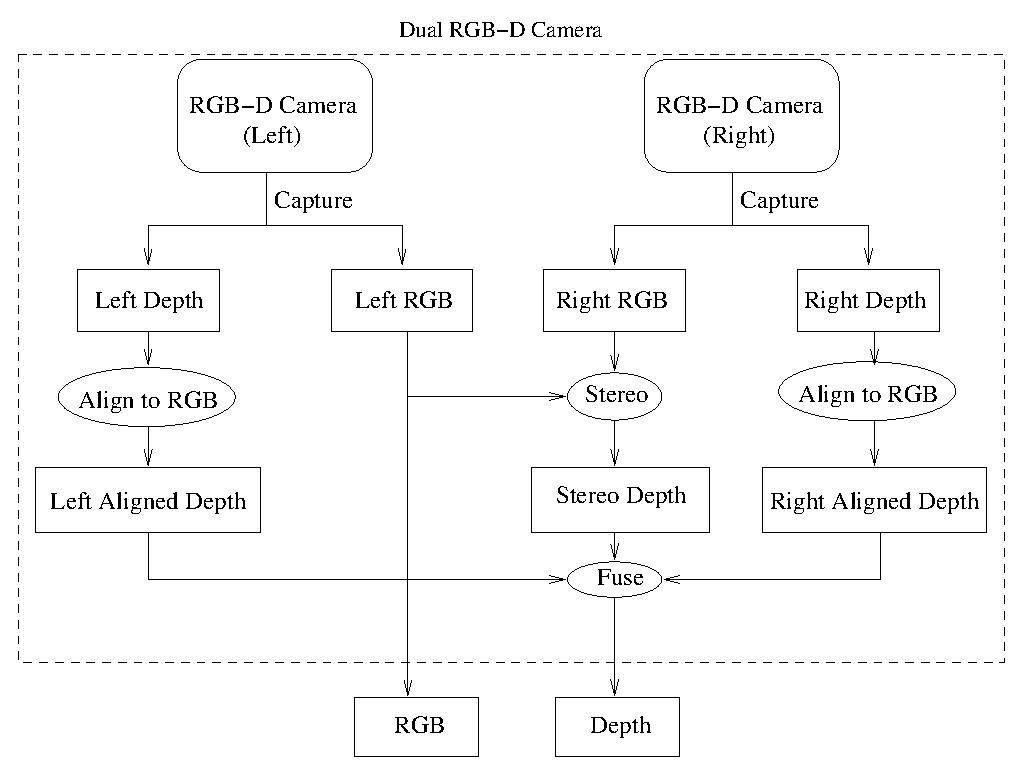
\includegraphics[width=14cm]{dual_rgbd_struct}
  \caption{对偶RGB-D相机内部原理图}
  \label{fig:dual_rgbd_struct}
\end{figure}

从外部使用来看,对偶RGB-D相机也输出一张彩色图、一张深度图。输出的彩色图就是从上相机采集到的彩色图;输出的深度图是由三张深度图融合而成,并且与输出的彩色图相对齐,对齐的意思是彩色图和深度图相同图像坐标下的颜色信息和深度信息对应的实际物理世界中相同的一点,对齐的意义在于方便后续的一些图像处理的算法。

从内部实现来看,主要涉及到三个部分:
\begin{itemize}
\item 将深度图与输出的彩色图对齐(Align to RGB)
\item 利用上相机采集的彩色图和下相机采集的彩色图,通过双目匹配算法形成一张新的深度图
\item 融合上相机对齐后的深度图、下相机对齐后的深度图和双目匹配得到的深度图
\end{itemize}
将深度图与彩色图对齐,相对来讲实现还是比较简单的,对齐深度图的具体流程如算法\ref{alg:align}所示。
\begin{algorithm}[!ht]
  \caption{Align Depth Frame}
  \label{alg:align}
  \KwIn{Raw Depth Frame $Raw\_D_{dh\times dw}$}
  \KwOut{Aligned Depth Frame $Aligned\_D_{ch\times cw}$}
  \For {p in $Aligned\_D$} {
    $p = 0$
  }
  \For {dy = 1; dy <= dh; ++dy} {
    \For {dx = 1; dx <= dw; ++dx} {
      通过深度相机内参将点$(dx, dy)$反投影到三维空间一点$\tensor*[^D]{\bm{X}}{}$\;
      坐标变换$\tensor*[^R]{\bm{X}}{} = \tensor*[^R_D]{\bm{R}}{}\tensor*[^D]{\bm{X}}{} + \tensor*[^R_D]{\bm{t}}{}$\;
      通过彩色相机内参将点$\tensor*[^R]{\bm{X}}{}$投影变换到彩色图像坐标系下一点$(cx, cy)$\;
      \If {cx in $(0, cw]$ and cy in $(0, ch]$} {
        $Aligned\_D(cx, cy) = Raw\_D(dx, dy)$\;
      }
    }
  }
\end{algorithm}
算法\ref{alg:align}主要将深度图中每个点的图像坐标利用该点的深度信息反投影变换到实际三维空间中一点,然后将该点坐标变换到彩色相机坐标系下,最后通过彩色相机的内参将该点在彩色相机坐标系下的三维坐标投影变换到彩色图像上的二维坐标。实际对齐三张深度图时,对于上相机深度图对齐到上相机彩色图,需要分别知道上相机深度相机和彩色相机的内参和畸变参数以及深度相机与彩色相机之间的齐次变换关系(通过相机标定这些参数都可以得到);双目匹配得到的深度图理论上可以有两张,一张与上相机校准后的彩色图像对齐,另一张与下相机校准后的彩色图像对齐,简单起见,选择与上相机对齐的深度图,然后通过上相机校准所使用的旋转矩阵的逆矩阵即可得到与原上相机彩色图像对齐的深度图;对齐下相机到上相机彩色图,除了要知道下相机标定的参数外,还需要知道下相机与上相机之间的齐次变换关系(通过对偶RGB-D相机的标定得到)。

利用上下相机采集到的两张彩色图获取深度信息主要分为三步:
\begin{itemize}
\item 分别对两张原始图像进行校准
\item 在校准后的两张图像上通过匹配算法得到视差图
\item 通过视差图获取深度图
\end{itemize}
对两张原始图像进行校准主要通过双目相机的标定实现,使得校准后的两张图像的极线对齐,如图\ref{fig:stereo_images}所示,
\begin{figure}[!ht]
  \centering
  \subfloat[上相机原始图像]{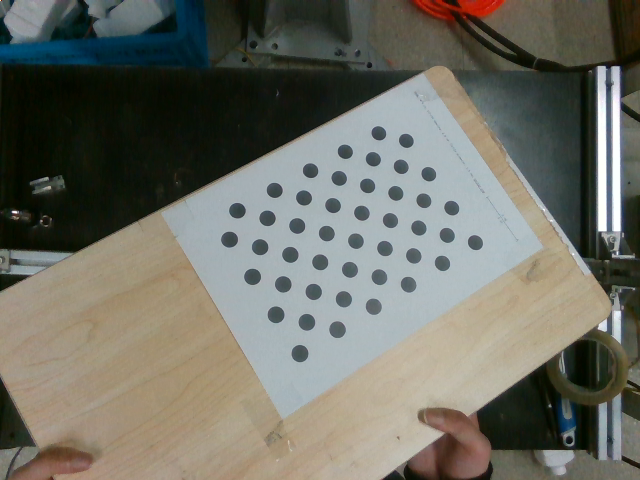
\includegraphics[width=7cm]{left_raw_image}}
  \hfill
  \subfloat[上相机校准后图像]{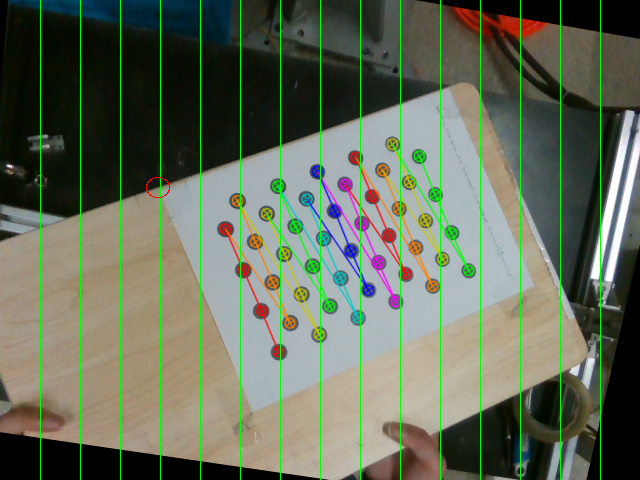
\includegraphics[width=7cm]{left_rectified_image}}
  \vfill
  \subfloat[下相机原始图像]{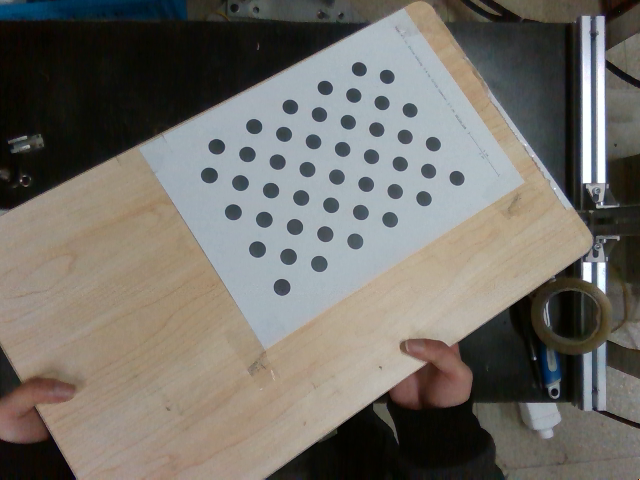
\includegraphics[width=7cm]{right_raw_image}}
  \hfill
  \subfloat[下相机校准后图像]{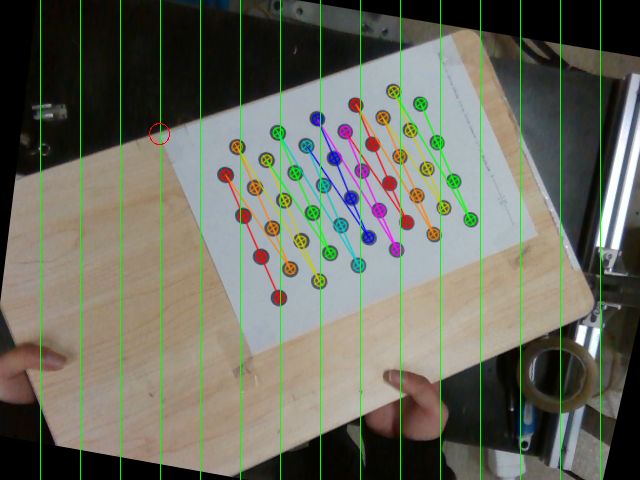
\includegraphics[width=7cm]{right_rectified_image}}
  \caption{双目相机原始图像和校准后图像}
  \label{fig:stereo_images}
\end{figure}
其中绿色的直线便是图像对齐后的部分极线,可以看出校准后的图像的对应点都分布在对齐的极线上(如图中用红色圈出的一对对应点所示),这样使得双目的匹配算法的搜索从二维缩小到了一维,只需要在极线上找对应点即可,能更快更稳定地在两张图中找到对应点。双目匹配算法使用的是ELSA算法\cite{Geiger2010},通过ELSA算法可以从两张校准后彩色图像上得到对应的视差图,视差图到深度图的变化可以通过公式\ref{eq:reprojection}得到:
\begin{equation}
  \label{eq:reprojection}
  z = \frac{\prescript{\{T,\,R\}}{}{f}B}{-(\prescript{\{T,\,R\}}{}{v_0}-\prescript{\{B,\,R\}}{}{v_0}) + \prescript{\{T,\,R\}}{}{d}}
\end{equation}
其中上标\{$T,R$\}(Top,RGB)表示上相机的RGB摄像头,\{$B,R$\}(Bottom,RGB)表示下相机的RGB摄像头,$B$表示基线长度,$\prescript{\{T,\,R\}}{}{d}$表示视差。一般地,会人为地校准过程中使得$\prescript{\{T,\,R\}}{}{v_0}-\prescript{\{B,\,R\}}{}{v_0}=0$,从而公式\ref{eq:reprojection}可以简化为:
\begin{equation}
  \label{eq:reprojection_simple}
  z = \frac{\prescript{\{T,\,R\}}{}{f}B}{\prescript{\{T,\,R\}}{}{d}}
\end{equation}

融合上相机对齐后的深度图、下相机对齐后的深度图以及双目匹配得到的深度这三张深度图的算法首先做的是分别对这三张深度图进行预处理,填补一些深度缺失的像素,因为对齐后的深度图和双目匹配得到的深度图深度信息都有细微的缺失,填补深度信息缺失的方法如算法\ref{alg:fill_hole}所示。
\begin{algorithm}[!ht]
  \caption{Fill Holes in Depth Frame}
  \label{alg:fill_hole}
  \KwIn{Depth Frame $D_{h\times w}$}
  \KwOut{Filled Depth Frame $FD_{h\times w}$}
  \For {y = 1; y <= h; ++y} {
    \For {x = 1; x <=w ; ++x} {
      \If {valid($D_{x,y}$)} {
        $FD_{x,y} = D_{x,y}$\;
      } \Else {
        $FD_{x,y}$= NAN\;
        bool leftTop = valid($D_{x-1, y-1}$) or valid($D_{x, y-1}$) or valid($D_{x-1, y}$)\;
        bool leftBottom = valid($D_{x-1, y+1}$) or valid($D_{x, y+1}$) or valid($D_{x-1, y}$)\;
        bool rightTop = valid($D_{x+1, y-1}$) or valid($D_{x, y-1}$) or valid($D_{x+1, y}$)\;
        bool rightBottom = valid($D_{x+1, y+1}$) or valid($D_{x, y+1}$) or valid($D_{x+1, y}$)\;
        \If {leftTop and leftBottom and rightTop and rightBottom} {
          validPoints = \{\}\;
          \For {dy = -1; dy <=1; ++dy} {
            \For {dx = -1; dx <=1; ++dx} {
              \If {valid($D_{dx, dy}$)} {
                push back $D_{x, y}$ to validPoints\;
              }
            }
          }
          \If {max(validPoints) - min(validPoints) < 0.05} {
            $FD_{x,y}$= mean(validPoints)\;
          }
        }
      }
    }
  }
\end{algorithm}
算法\ref{alg:fill_hole}主要实现对于深度缺失的点,将检查其周围的深度信息,当其四个角上都有有效的深度信息时,并且周围有效深度信息的极值小于一定阈值时,会用周围有效深度信息的均值填充该缺失的点。实际的效果如图\ref{fig:fill_hole}所示。
\begin{figure}[!ht]
  \centering
  % @TODO: fill hole 效果图
  \caption{填补深度信息缺失算法效果图}
  \label{fig:fill_hole}
\end{figure}
分别对深度图进行预处理后,将会对三张深度图进行线性叠加得到最终的深度图,基本叠加的公式如\ref{eq:linear}所示。
\begin{equation}
  \label{eq:linear}
  d_{fuse} = \frac{w_1d_{left} + w_2d_{right}+w_3d_{stereo}}{w_1+w_2+w_3}
\end{equation}
其中$w_1,w_2,w_3$分别表示上相机深度、下相机深度以及双目匹配深度的权重,SR300相机得到深度的精度比双目计算得到的深度要高,所以实际使用时$w_1,w_2$要比$w_3$大许多。融合三张深度图的理论相对简单,但实际上,三张深度图的深度信息并非都会永远有效,因此根据实际情况实际的融合算法如\ref{alg:fuse}所示。
\begin{algorithm}[!ht]
  \caption{Fuse Depth Frames}
  \label{alg:fuse}
  \KwIn{leftDepth, rightDepth, stereoDepth}
  \KwOut{fuseDepth}
  Initialize w1,w2,w3\;
  \For {(d1,d2,d3,d4) in (leftDepth, rightDepth, stereoDepth, fuseDepth)} {
    validDepth = [], validWeight = []\;
    \For {i = 1 to 3} {
      \If {di is valid} {
        push back di to validDepth, wi to validWeight\;
      }
    }
    \If {size of validDepth == 0} {
      d4 = NAN\;
    } \ElseIf {size of validDepth == 1} {
      d4 = validDepth[1]\;
    } \ElseIf {size of validDepth == 2 } {
      \If {extremum of validDepth < 0.03} {
        d4 = validDepth $\cdot$ validWeight / sum of validWeight\;
      } \Else {
        d4 = NAN\;
      }
    } \Else {
      mediumDepth = medium(validDepth)\;
      d4 = 0, sum = 0\;
      \For {(d,w) in (validDepth, validWeight)} {
        \If {abs(d-mediumDepth) < 0.03} {
          d4 += d*w\;
          sum += w\;
        }
      }
      \If {sum > 0} {
        d4 = d4 / sum\;
      } \Else {
        d4 = NAN\;
      }
    }
  }
\end{algorithm}
算法\ref{alg:fuse}不仅考虑了深度缺失的情况,对于深度信息差值过大的情况也进行了处理。实际处理的效果如图\ref{fig:fuse}所示。
\begin{figure}[!ht]
  \centering
  % @TODO 深度融合算法效果图
  \caption{深度融合算法效果图}
  \label{fig:fuse}
\end{figure}

\subsection{对偶RGB-D相机的标定流程}
对偶RGB-D相机的标定流程可以分为三步:
\begin{enumerate}[Step 1]
\item 分别标定好单个RGB-D相机
\item 标定出两个彩色相机之间的齐次变换关系
\item 标定出矫正彩色图像的旋转矩阵以及矫正后图像的投影矩阵
\end{enumerate}
单个RGB-D相机的标定在\ref{sec:rgb-d_calibration}小节中已经详细叙述过了,分别标定完单个RGB-D相机后,后面的步骤其实就等价于双目标定了。双目的几何结构如图\ref{fig:stereo}所示,
\begin{figure}[!ht]
  \centering
  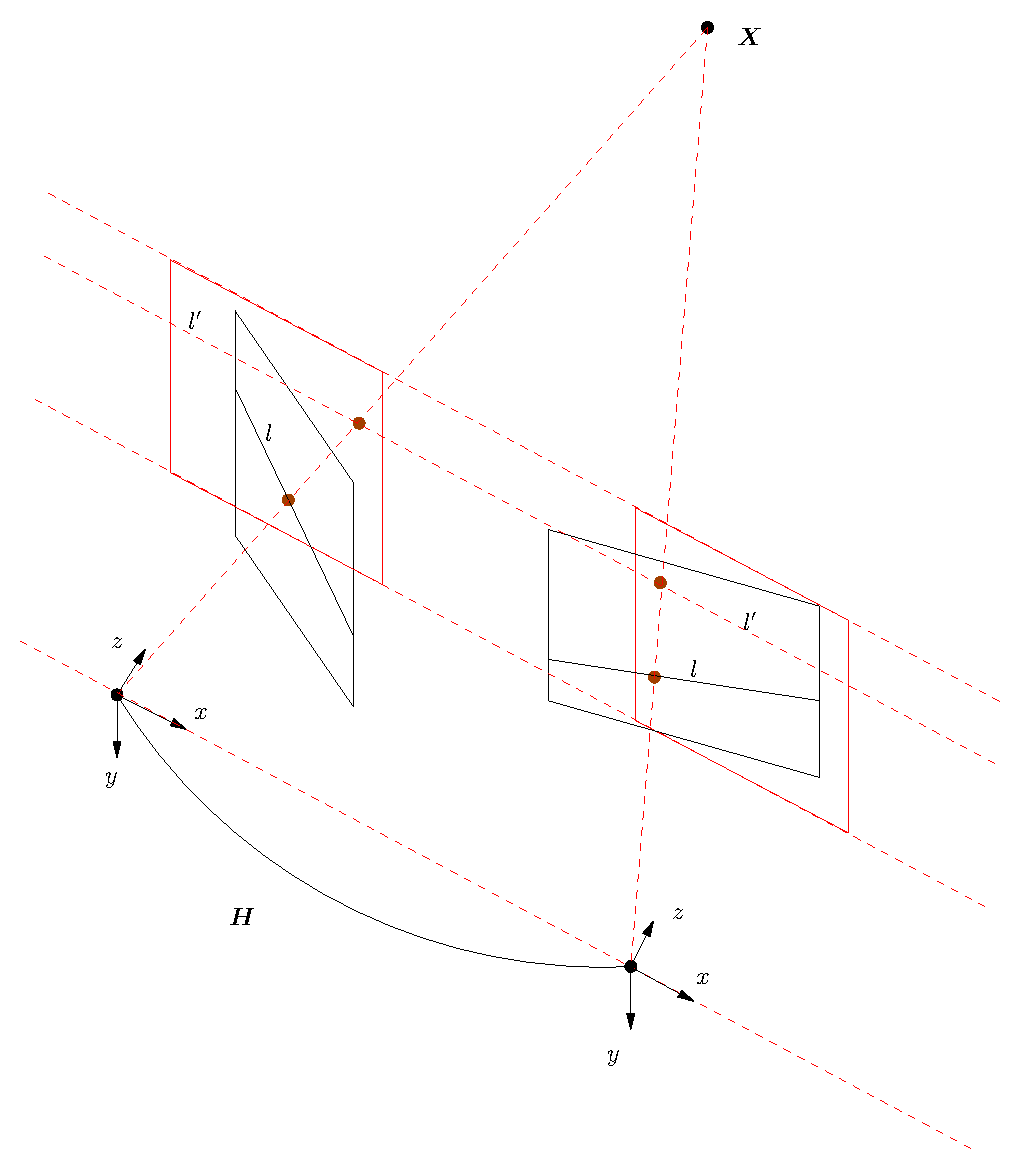
\includegraphics[width=14cm]{stereo}
  \caption{双目几何结构}
  \label{fig:stereo}
\end{figure}
标定出两个彩色相机之间的齐次变换关系,即图\ref{fig:stereo}中的$H$,简单地可以通过8点法\cite{Sur2008}先求出基础矩阵(Fundamental Matrix)$F$,即所谓的“弱标定”,然后根据相机的内参矩阵可求得本质矩阵(Essential Matrix)$E$:
\begin{equation}
  E = K^{T}FK'
\end{equation}
其中$K$和$K'$分别是两个相机的内参矩阵。求得本质矩阵后可以通过奇异值分解求得齐次变换矩阵的旋转矩阵$R$和平移向量$T$:
\begin{equation}
  \left\{\begin{array}{ccc}
    E &=& U\Sigma V^T \\
    R &=& U\bm{R}_Z^T(\frac{\pi}{2})V^T \\
    \left[T\right]_{\times} &=& U\bm{R}_Z^T(\frac{\pi}{2})\Sigma U^T
  \end{array}
  \right.
\end{equation}
其中$\bm{R}_Z(\theta)$表示绕$Z$轴旋转$\theta$角的旋转矩阵,$\left[T\right]_{\times}$的定义如下:
\begin{equation}
  \left[T\right]_{\times} = \left[
    \begin{array}{ccc}
      0&-T_z&T_y\\
      T_z&0&-T_x \\
      -T_y&T_x&0
    \end{array}
  \right]
\end{equation}
矫正彩色图像的旋转矩阵会将图\ref{fig:stereo}中黑色线框的图像平面变换到红色线框的图像平面上,使得对应点在两张图像的同一条极线上。矫正彩色图像的旋转矩阵的计算参考文献\cite{Loop2001},此步标定完最终可以得到:
\begin{itemize}
\item 两个相机的矫正旋转矩阵$R_1$,$R_2$
\item 两个矫正坐标系下的投影矩阵$P_1$,$P_2$
\item 主相机\footnote{另外一个相机的投影变换矩阵也可以得到,但没有必要。}的投影变换矩阵$Q$
\end{itemize}
其中
\begin{equation}
  Q = \left[
    \begin{array}{cccc}
      1&0&0&-u_0 \\
       0&1&0&-v_0 \\
       0&0&0&f \\
       0&0&1/B&0
    \end{array}
    \right]
\end{equation}
包含了公式\ref{eq:reprojection_simple}由视差计算深度的所有参数。

\section{RGB-D相机精度测量实验}
% @TODO: 精度测量实验

\section{本章小结}
% @TODO: 本章小结

\chapter{3D目标检测与位姿估计算法}
\label{chap:pose}
本章介绍了本文所设计的基于RGB-D图像的3D目标检测和位姿估计算法3D-MRAI(3D Mask R-CNN with Angle-fixed-4PCS and ICP),该算法根据所提供目标的CAD模型,可以在RGB-D图中检测出目标,并给出目标的位姿。所提出的3D-MRAI算法主要有两个模块构成:检测模块和匹配模块。检测模块基于Mask R-CNN\cite{He2017}实现在3D点云中定位目标,匹配模块通过匹配目标3D模型和由检测模块定位的目标点云实现对目标的位姿估计。为了评价所设计的3D-MRAI算法的性能,本章还设计了相关实验,并与同类算法相比较,从算法的检测准确度、位姿精度和时间性能三个方面分析了算法性能。

\section{3D-MRAI框架设计}
本文设计的3D-MRAI算法主要解决三维空间中的目标检测和位姿估计问题,根据输入的RGB-D图像,输出图像中的目标和其在三维空间中的位姿,区别于常见的2D目标检测算法(2D目标检测算法往往只给出目标的种类和其在图像坐标中的Bounding box或者Mask)。给出目标在三维空间中的位姿的意义十分巨大,尤其在机器人领域中,图像层面的结果往往难以满足要求,但同时算法的难度也很大。

一些给出3D目标位姿的传统算法,如3DMatch\cite{zeng20163dmatch},3DMatch通过匹配局部几何特征来计算目标的位姿,缺点是对采集的3D数据质量要求很高,往往需要使用激光采集,因此整个识别过程的时间很久;通过SIFT描述子来匹配目标位姿\cite{dias2015sift}也是一种方法,但其对纹理较少的物体往往难以匹配,效果很差;另外如LINEMOD\cite{hinterstoisser2012gradient}和MOPED\cite{collet2011moped}这些位姿估计框架,在某些情况下如目标在平整的桌面上并且光照条件较好的情况下才能取得满意的效果。因此,传统的一些3D目标位姿估计算法往往难以在实际中具体应用,为此,本文设计一种鲁棒性和准确率都较高的3D目标检测和位姿估计算法3D-MRAI。

所设计的3D-MRAI算法的框架如图\ref{fig:detect-pose}所示,
\begin{figure}[ht]
  \centering
  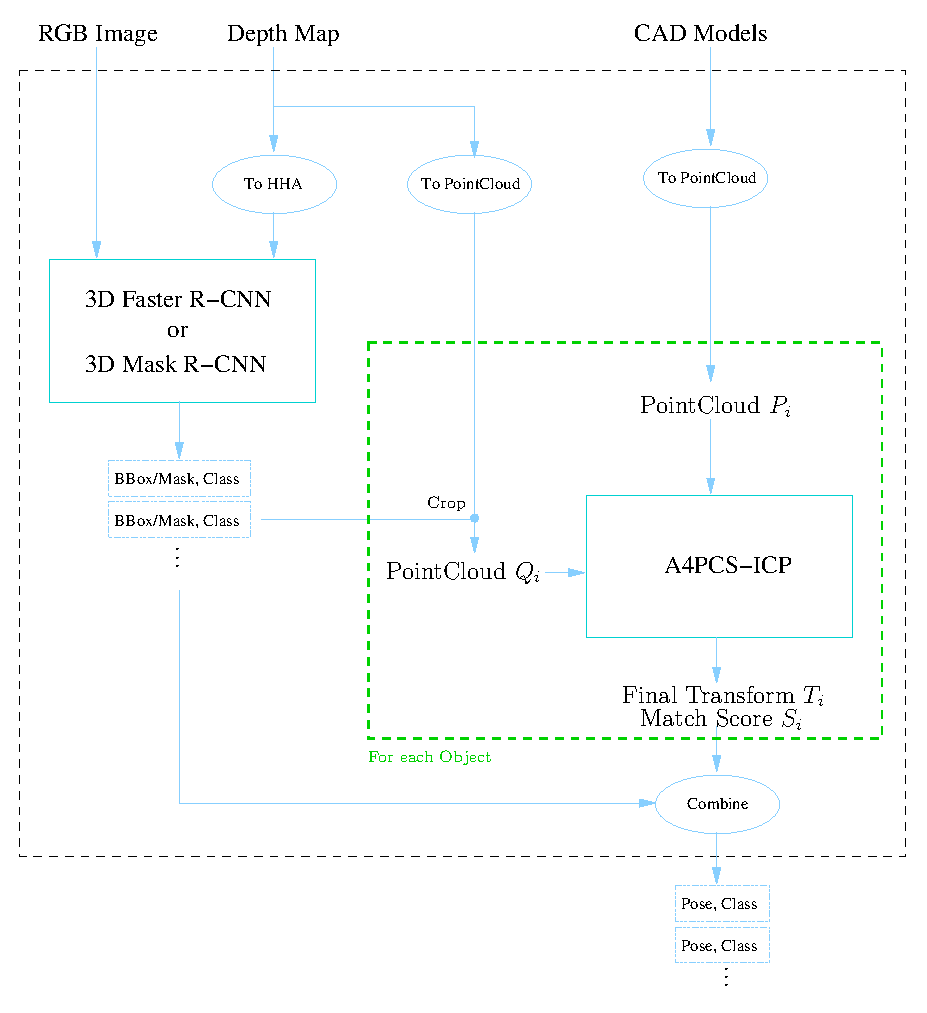
\includegraphics[width=12cm]{detect-pose}
  \caption{3D-MRAI算法框架}
  \label{fig:detect-pose}
\end{figure}
从图\ref{fig:detect-pose}可以看出算法的输入是RGB图像、深度图,以及目标物体的CAD模型,输出是图像中检测到的目标的位姿。所设计的3D-MRAI算法的核心部分为两个模块:检测模块和匹配模块。检测模块通过引入HHA(Horizontal disparity, Height above ground, Angle with gravity)和STN(Spatial Transformer Network)将Faster R-CNN\cite{Ren}和Mask R-CNN\cite{He2017}扩展到RGB-D图像上来,使其检测缺少纹理目标的准确率大大提升;匹配模块在4PCS算法\cite{aiger20084}的基础上,对其进行改进,减少了算法运算时间,并通过ICP算法\cite{besl1992method}迭代提高匹配精度。两个模块完成的主要功能如下:
\begin{itemize}
\item {\kai 检测模块}:在RGB-D图中检测出目标,得到目标BBox(Bounding Box)或者Mask
\item {\kai 匹配模块}:将目标3D模型与由BBox/Mask分割的目标点云进行匹配,得到目标位姿
\end{itemize}

\section{检测模块}
\label{sec:detector}
\subsection{模块框架设计}
本文所设计的检测模块有两种:一种基于Faster R-CNN,另外一种基于Mask R-CNN。两种模块的输出不同,基于Faster R-CNN的检测模块在RGB-D图中输出的是目标的Class和BBox;基于Mask R-CNN的检测模块输出的是目标的Class、BBox和Mask。从模块输出来看,基于Faster R-CNN的检测模块是基于Mask R-CNN的检测模块的子集。在设计之初,基于Faster R-CNN的检测模块先被设计出来,由于基于Faster R-CNN的检测模块的输出只有Class和BBox,对于普通物体通过BBox分割目标点云再输入到匹配模块进行匹配并没有什么问题,但是,当所要检测的物体是细长类型的,在某些位姿下,如图\ref{fig:bbox-segment}所示BBox内的大部分像素都不是目标物体,此时通过该BBox分割得到的目标点云也包含了许多不属于该目标的点,这样的点云输入到匹配模块很难进行正确的匹配。
\begin{figure}[ht]
  \centering
  \subfloat[检测模块输出的BBox示意图]{
    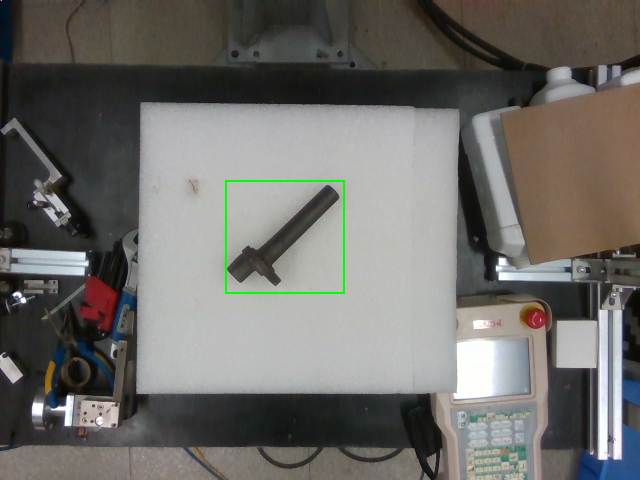
\includegraphics[width=6cm]{bbox-segment}
  }
  \hskip1cm
  \subfloat[根据BBox分割得到的点云]{
    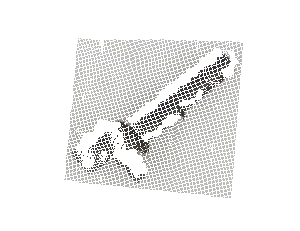
\includegraphics[width=6cm]{bbox-segment-cloud}
  }
  \caption{由BBox分割点云效果图}
  \label{fig:bbox-segment}
\end{figure}

\begin{figure}[ht]
  \centering
  \subfloat[检测模块输出的Mask示意图]{
    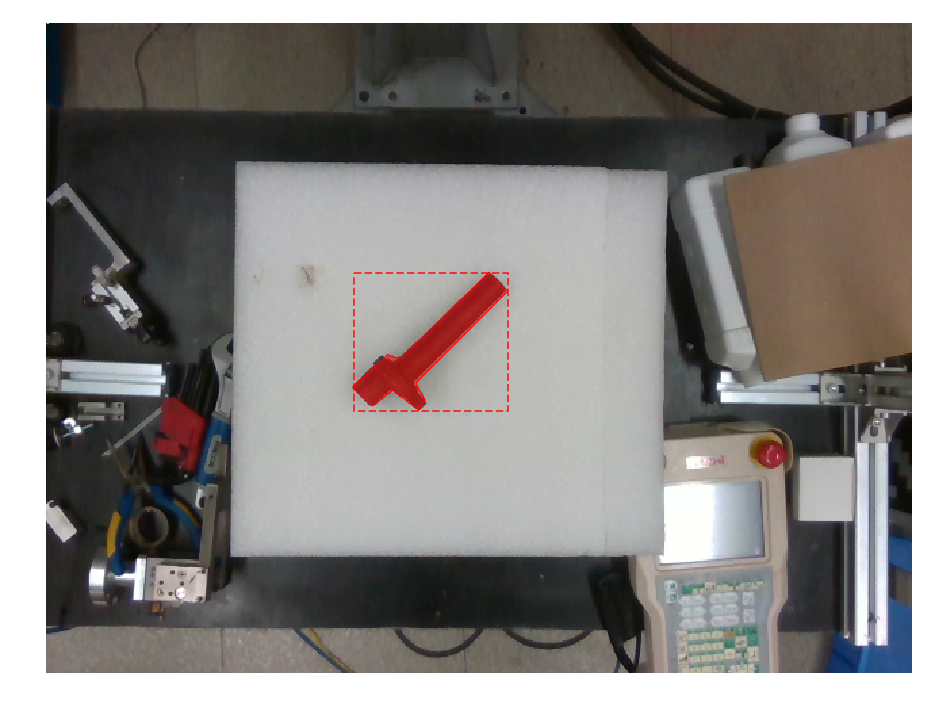
\includegraphics[width=6cm]{mask-segment}
  }
  \hskip1cm
  \subfloat[根据Mask分割得到的点云]{
    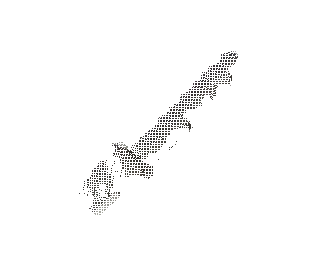
\includegraphics[width=6cm]{mask-segment-cloud}
  }
  \caption{由Mask分割点云效果图}
  \label{fig:mask-segment}
\end{figure}
为了解决这一个问题,本文参考Mask R-CNN对Faster R-CNN的改进,设计了基于Mask R-CNN的检测模块,通过Mask R-CNN检测输出的Mask分割点云,有效的解决了利用BBox分割细长物体时造成目标点云包含过多不属于目标的点的问题,如图\ref{fig:mask-segment}所示。但是,基于Faster R-CNN的检测模块也有其存在的必要,因为基于Mask R-CNN的检测模块的运算时间要大于基于Faster R-CNN的检测模块,所以,如果考虑算法的时间性能,对于细长物体建议使用基于Mask R-CNN的检测模块,除此之外使用基于Faster R-CNN的检测模块。

基于Faster R-CNN的检测模块的框架如图\ref{fig:3d_faster_rcnn}所示,基于Mask R-CNN的检测模块的框架如图\ref{fig:3d_mask_rcnn}所示。
\begin{figure}[ht]
  \centering
  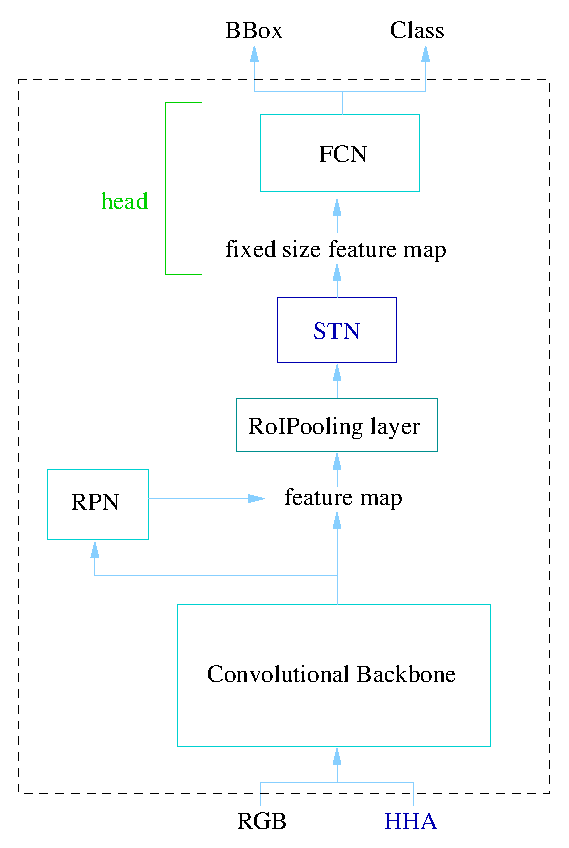
\includegraphics[width=8cm]{faster_rcnn_module}
  \caption{基于Faster R-CNN的检测模块}
  \label{fig:3d_faster_rcnn}
\end{figure}
\begin{figure}[ht]
  \centering
  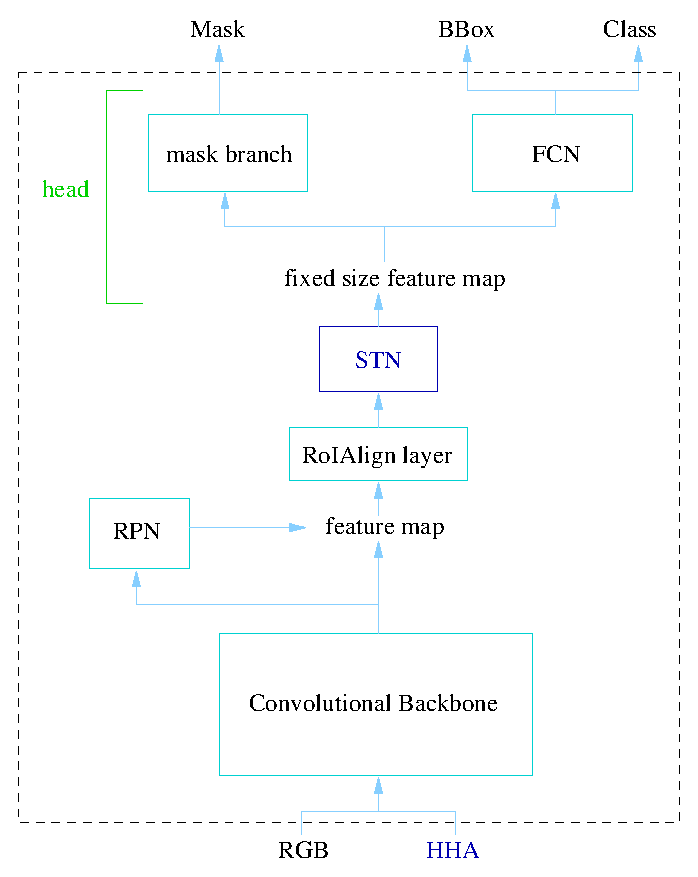
\includegraphics[width=10cm]{mask_rcnn_module}
  \caption{基于Mask R-CNN的检测模块}
  \label{fig:3d_mask_rcnn}
\end{figure}
两个检测模块对Faster R-CNN和Mask R-CNN的改进相同,因此本文主要介绍对Mask R-CNN的改进,对Faster R-CNN的改进类似。

\subsection{对Mask R-CNN的改进}
Mask R-CNN是一个2D目标检测的深度神经网络,其网络结构如图\ref{fig:mask_rcnn}所示。
\begin{figure}[ht]
  \centering
  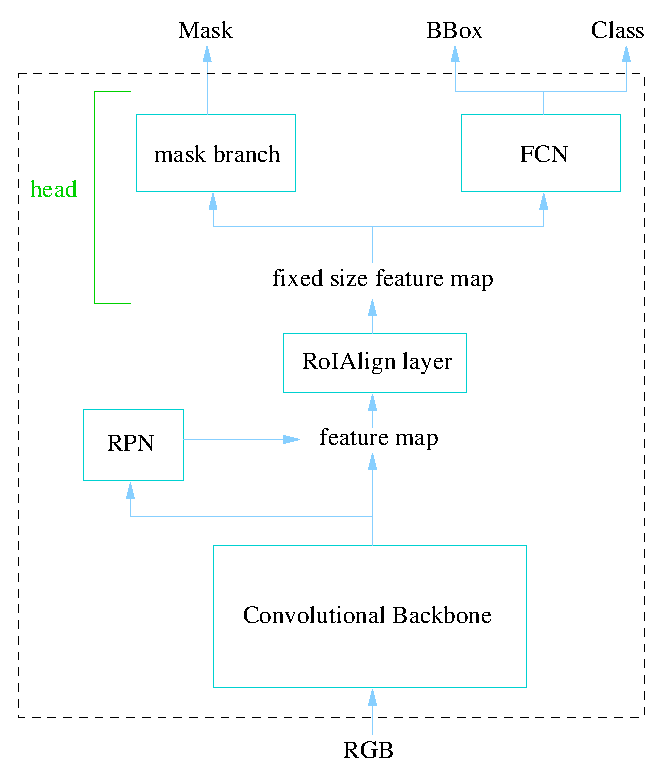
\includegraphics[width=10cm]{mask_rcnn}
  \caption{Mask R-CNN网络结构}
  \label{fig:mask_rcnn}
\end{figure}
Mask R-CNN在Faster R-CNN的基础上通过增加一个Mask分支,使得网络不仅可以输出目标的Class和BBox,还可以输出目标的Mask。除此之外,Mask R-CNN还通过改用ResNeXt-101+FPN强化了Faster R-CNN中的特征提取网络(convolutional backbone),其中ResNeXt\cite{xie2017aggregated}是残查网络ResNet\cite{he2016deep}的改进, ResNeXt结构可以在不增加参数复杂度的前提下提高准确率,同时还减少了超参数的数量;FPN(Feature Pyramid Networks)\cite{lin2017feature}利用了深度卷积神经网络固有的多尺度、多层级的金字塔结构去构建特征金字塔网络来提升检测的准确度。Mask R-CNN还提出了ROIAlign层,替换掉Faster R-CNN中的ROIPooling层,从而解决ROIPooling造成的像素不对齐问题,实现预测Pixel级别的Mask。

本文所设计的检测模块对Mask R-CNN的改进主要有两点:
\begin{itemize}
\item 将深度图转化为HHA图与RGB图一起输入到网络
\item 在ROIAlign层后面增加了STN
\end{itemize}

Mask R-CNN网络本来的输入是RGB图,经过实验测试,本文发现单单通过RGB图Mask R-CNN难以检测一堆缺少纹理的物体(Textureless Object)。对于缺少纹理的物体虽然在RGB图中难以检测,但是其在深度图中信息还没有有效利用,所以可以尝试将RGB图和深度图相结合。

从2012年AlexNet\cite{Krizhevsky2012}在ImageNet\cite{imagenet}数据集上的应用开始,深度学习在彩色图上的应用已经相当成熟,但深度学习在深度图上的应用还比较少,如何使用CNN在深度图上提取特征是一个值得探讨的问题,是将深度图直接作为一个通道使用CNN提取特征?还是将深度图变换到三维坐标(x,y,z),然后再在这三个通道上通过CNN提取特征?经过实验和相关调研,本文发现将深度图转换为HHA图后进行训练的模型有较高的准确率\cite{Gupta2014},因此本文将深度图转换为HHA三个通道,然后再通过CNN提取特征。HHA三个通道的分别为:
\begin{itemize}
\item 水平方向上视差(Horizontal disparity)
\item 距离地面的高度(Height above ground)
\item 法向量与重力的夹角(Angle with gravity)
\end{itemize}

\emph{Horizontal disparity}:深度图到视差的转换相对来说十分简单,理论上视差与深度呈倒数关系,因此水平方向上的视差计算具体如算法\ref{alg:hd}所示。
\begin{algorithm}[!ht]
  \caption{计算水平方向上视差}
  \label{alg:hd}
  \KwIn{Depth Frame $D_{h\times w}$}
  \KwOut{Horizontal disparity Frame $H_{h\times w}$}
  $h_{floor} = 1 / d_{ceil}, h_{ceil} = 1 / d_{floor}$\;
  \For {$y\leftarrow 1$ \KwTo $h$} {
    \For {$x\leftarrow 1$ \KwTo $w$} {
      $H[y, x] = 1 / D[y, x]$\;
      $H[y, x] = (H[y, x] - h_{floor}) / (h_{ceil} - h_{floor})$\;
    }
  }
\end{algorithm}

\emph{Height above ground}:计算距离地面的高度首先要确定一个世界坐标系,然后得到世界坐标系到相机坐标系的旋转矩阵$\prescript{W}{C}{R}$和平移向量$\prescript{W}{C}{T}$,最后通过坐标变换得到距离地面的高度,具体如算法\ref{alg:hg}所示。
\begin{algorithm}[!ht]
  \caption{计算距离地面的高度}
  \label{alg:hg}
  \KwIn{Point Cloud $P_{h\times w}$}
  \KwOut{Hight Frame $H_{h\times w}$}
  \For {$y\leftarrow 1$ \KwTo $h$} {
    \For {$x\leftarrow 1$ \KwTo $w$} {
      $p =  \prescript{W}{C}{R}P[y, x] + \prescript{W}{C}{T}$\;
      $H[y, x] = p.z$\;
    }
  }
\end{algorithm}

\emph{Angle with gravity}:法向量与重力的夹角的计算相对来说稍微复杂一点,重力的方向在工作区间内一般与所设的世界坐标系的$z$轴负方向相同,因此原问题就是求法向量与世界坐标系$z$轴负方向之间的夹角。参考文献\cite{Gupta2013},首先计算深度图中每个点上的法向量,计算点云中一点$p_0$的法向量$\vec{n}$的简单思路如下:
\begin{itemize}
\item 找出距离点$p_0$最近的$k$个点:$p_1, p_2,...p_k$
\item 通过最小二乘在点$\{p_i|i = 0, 1, \ldots , k\}$中拟合出平面$Ax + By + Cz + D = 0$
\item 点$p_0$的法向量$\vec{n} = [A, B, C]^T$
\end{itemize}
考虑到所采集的深度图转换的点云是有序的(Organized Point Cloud),意味着坐标索引相近的点实际物理距离也相近,因此找出距离点$p_0$最近的$k$个点可以通过选取点$p_0$坐标索引附近的点代替,具体地,记点$p_0$在深度图中图像坐标为$(x_0, y_0)$,取点集$\bm{S} = \{p_i|x_0 - R \leq x_i \leq x_0 + R , y_0 -R \leq y_i \leq y_0 + R\}$,其中$R$是选取区域的半径。得到法向量后计算法向量与世界坐标$z$轴负方向的角度就十分简单了,整个计算法向量与重力的夹角的算法如\ref{alg:angle}所示。
\begin{algorithm}[!ht]
  \caption{计算法向量与重力的夹角}
  \label{alg:angle}
  \KwIn{Point Cloud $P_{h\times w}$}
  \KwOut{Angle Frame $A_{h\times w}$}
  \For {$y\leftarrow 1$ \KwTo $h$} {
    \For {$x\leftarrow 1$ \KwTo $w$} {
      Calculate surface normal $\prescript{C}{}{\vec{n}}$ at point $P[y,x]$\;
      $\prescript{W}{}{\vec{n}} =  \prescript{W}{C}{R}\prescript{C}{}{\vec{n}} + \prescript{W}{C}{T}$\;
      $A[y, x] = arccos(-(\vec{n}\cdot\vec{oz}) / (|\vec{n}||\vec{oz}|))$\;
    }
  }
\end{algorithm}

计算完上述HHA三个通道后,为了计算和存储方便,分别将三个通道的值线性变换到0到255之间,可视化如图\ref{fig:hha}所示。
\begin{figure}
  \centering
  \subfloat[Depth frame]{
\includegraphics[width=4.5cm]{depth_frame}}
  \hskip5em
  \subfloat[HHA frame]{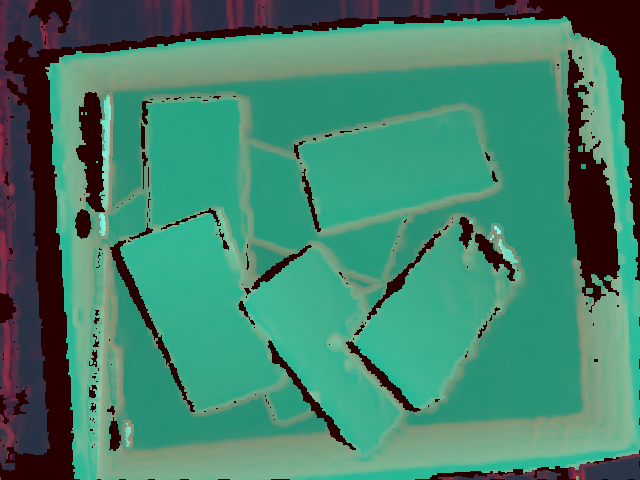
\includegraphics[width=4.5cm]{hha_frame}}
  \vfill
  \subfloat[Horizontal disparity frame]{
\includegraphics[width=4.5cm]{disparity_frame}}
  \hfill
  \subfloat[Height above ground frame]{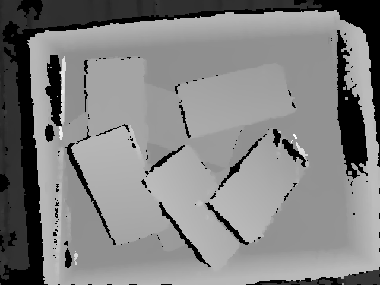
\includegraphics[width=4.5cm]{height_frame}}
  \hfill
  \subfloat[Angle with gravity frame]{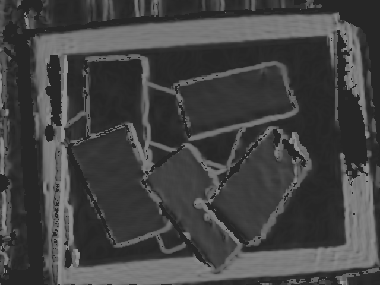
\includegraphics[width=4.5cm]{angle_frame}}
  \caption{HHA可视化效果图}
  \label{fig:hha}
\end{figure}

Mask R-CNN除了难以检测一堆缺少纹理的物体外,本文还发现Mask R-CNN训练得到的模型对物体旋转较为敏感,如图\ref{fig:cat}所示,
\begin{figure}[!ht]
  \centering
  \subfloat[检测旋转前的图片\label{fig:rotation1}]{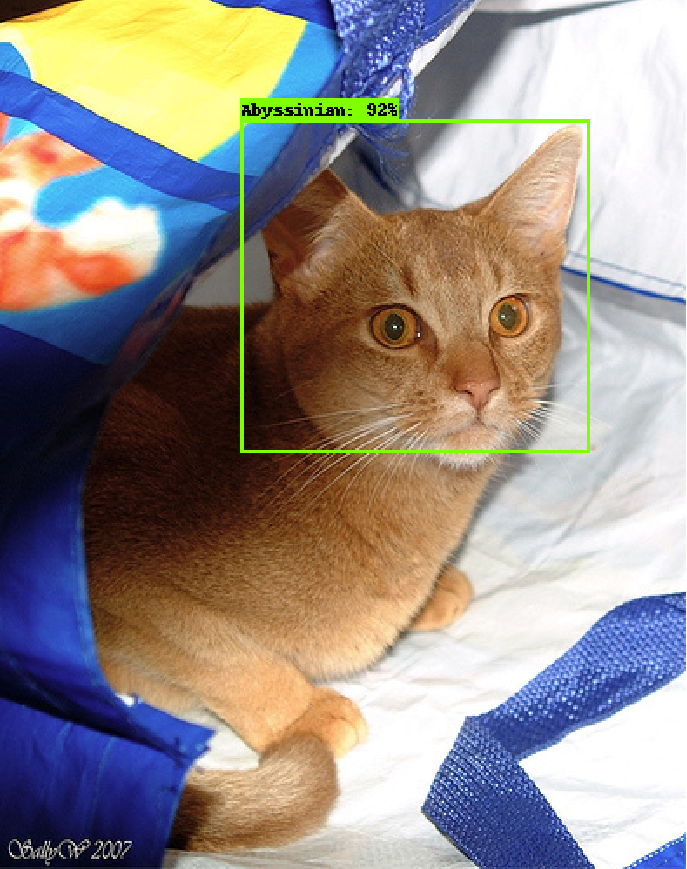
\includegraphics[width=4cm]{cat_up}}
  \hskip1em
  \subfloat[检测旋转后的图片\label{fig:rotation2}]{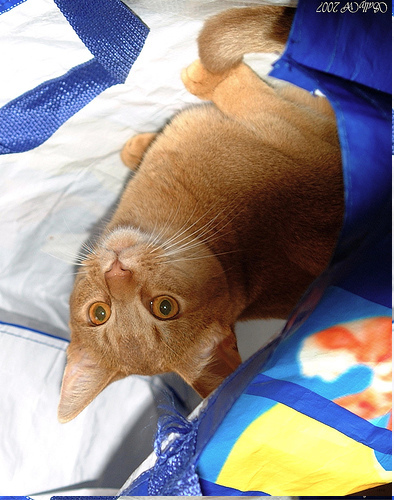
\includegraphics[width=4cm]{cat_down}}
  \caption{检测模型对旋转敏感}
  \label{fig:cat}
\end{figure}
其中图\ref{fig:rotation2}只是将图\ref{fig:rotation1}旋转了180度,由于CNN所提取的特征不具有旋转不变性,并且训练集中的图片宠物都是头朝上的,即使图\ref{fig:rotation1}在训练集中,将其旋转180度后,也无法从中检测出目标来。解决这个问题有两个思路:
\begin{itemize}
\item Data Augmentation
\item Spatial Transformer Network
\end{itemize}
Data Augmentation是通过对训练集中的图片进行旋转以获取不同角度的图片,通过这种方式增大数据集从而使得最终训练得到的模型对各种角度的图片都能识别;Spatial Transformer Network是一种特殊的网络结构,本文所使用的就这种方式。

Spatial Transformer Network是一个可微模块,根据输入的特征对其进行相应的空间变化,输出变换后的特征,如图\ref{fig:spatial_transformer_results}所示,
\begin{figure}[ht]
  \centering
  \subfloat{
    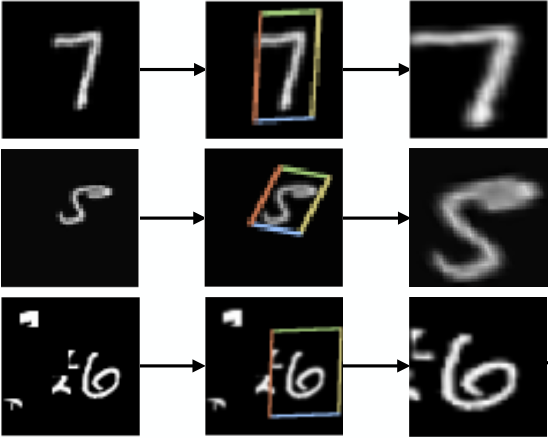
\includegraphics[width=6cm]{stn_results}
  }
  \hskip0.5cm
  \subfloat{
    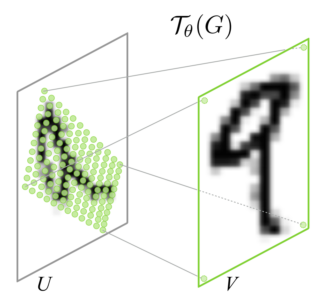
\includegraphics[width=6cm]{grid-generator}
  }
  \caption{Spatial Transformer Network效果图}
  \label{fig:spatial_transformer_results}
\end{figure}
输入特征$U$经过Spatial Transformer Network模块后输出特征$V$。Spatial Transformer Network模块具体可以分为三个部分,如图\ref{fig:spatial_transformer}。
\begin{figure}[ht]
  \centering
  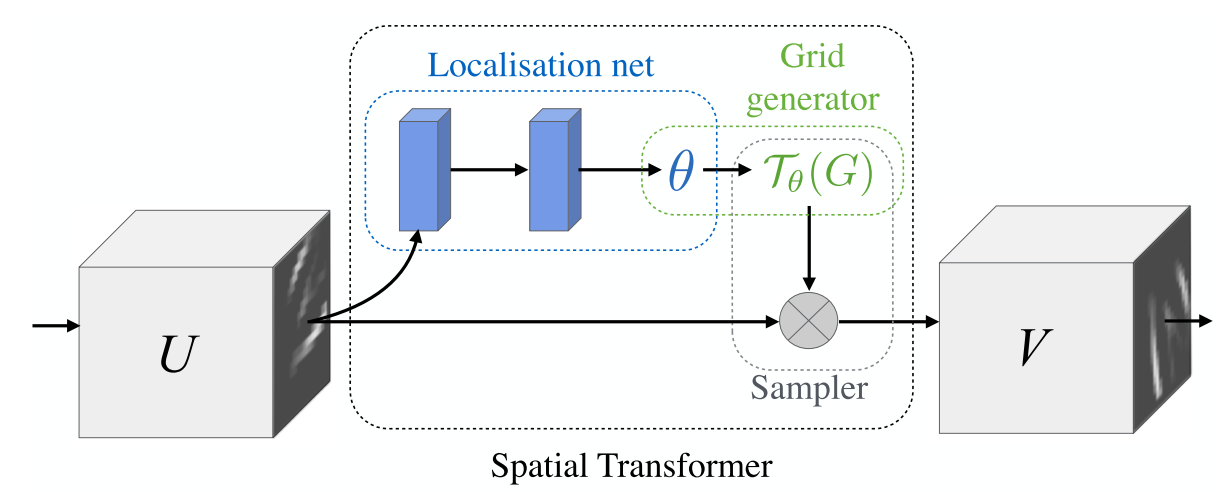
\includegraphics[width=12cm]{stn_structure}
  \caption{Spatial Transformer Network结构图}
  \label{fig:spatial_transformer}
\end{figure}
简单来讲,第一部分是一个定位网络(localisation network),输入特征$U$,输出需要进行空间变换的参数;第二部分是一个网格生成器(grid generator),根据空间变换的参数生成输入特征中需要变换的点的网格;第三部分是个采样器,根据网格生成器的输出对输入特征进行采样并进行空间变换,生成输出特征。

具体地,记定位网络的输入为特征$U\in \mathbb{R}^{H\times W\times C}$,其中$W,H,C$分别为长、宽和通道数,网络的输出为空间变化$\mathcal{T}_{\theta}$的参数$\theta$,参数$\theta$的个数由空间变换的类型决定,本文所采用的空间变换为2D仿射变换,则
\begin{equation}
  \mathcal{T}_\theta = \left[
    \begin{array}{ccc}
      \theta_{11}&\theta_{12}&\theta_{13}\\
      \theta_{21}&\theta_{22}&\theta_{23}
    \end{array}
    \right]
\end{equation}
定位网络内部可以由一些全连接层或者卷积层再加一个回归层组成。

网格生成器本质上就是在输入特征中选取需要进行空间变化的点,如图\ref{fig:spatial_transformer_results}中绿色点便是网格生成器所选取的点,记Spatial Transformer Network的输出特征为$V\in \mathbb{R}^{H'\times W'\times C}$,其中$W',H',C$分别为输出特征的长、宽和通道数,输出特征的通道数和输入特征的通道数相同,不能改变,并且空间变换$\mathcal{T}_{\theta}$将分别作用于输入$U$的各个通道以保证每个通道上的变换一致。并记点集$G = \{G_i|G_i = (x^t_i, y^t_i)\}$,其中$(x_i^s, y_i^s)$为输出特征图中点的坐标,由定位网络输出的参数$\theta$和$G$我们就可以在输入特征中确定需要进行空间变换的点的集合$\mathcal{T}_\theta(G)$:
\begin{equation}
  \left(
    \begin{array}{c}
      x_i^s\\
      y_i^s
    \end{array}
  \right) = \mathcal{T}_\theta(G_i) =
  \left[
    \begin{array}{ccc}
    \theta_{11}&\theta_{12}&\theta_{13}\\
    \theta_{21}&\theta_{22}&\theta_{23}
    \end{array}
  \right]
  \left(
    \begin{array}{c}
      x_i^t\\
      y_i^t\\
      1\\
    \end{array}
  \right)
\end{equation}
其中$(x_i^s, y_i^s)$是输入特征中点的坐标,也是图\ref{fig:spatial_transformer_results}中的绿色点。

采样器输入网格生成器生成的点集$\mathcal{T}_\theta$,和输入特征$U$,最终输出经过空间变换后的特征$V$,具体如公式\ref{eq:sampler}所示:
\begin{equation}
  \label{eq:sampler}
  V_i^c = \sum_n^H\sum_m^W{U_{nm}^ck(x_i^s-m;\Phi_x)k(y_i^s-n;\Phi_y)}\quad \forall i\in[1\ldots H'W']\quad \forall c\in[1\ldots C]
\end{equation}
其中$\Phi_{x}$和$\Phi_{y}$是采样核函数$k()$的参数,$U_{nm}^c$表示输入特征$U$在坐标$(n, m)$下第$c$个通道上的值,$V_i^c$表示输出特征在坐标$(x_i^t,y_i^t)$下第$c$个通道上的值。理论上可以使用任何采样核函数,只要可以对$x_i^s$和$y_i^s$求导,因为网络训练需要对公式\ref{eq:sampler}求导。以双线性采样核函数为例,公式\ref{eq:sampler}变为
\begin{equation}
  V_i^c = \sum_n^H\sum_m^W{U_{nm}^cmax(0, 1-|x_i^s-m|)max(0, 1-|y_i^s-n|)}
\end{equation}
则$V$对$U$和$G$的梯度为
\begin{equation}
  \frac{\partial V_i^c}{\partial U_{nm}^c} = \sum_n^H\sum_m^W{max(0, 1-|x_i^s-m|)max(0, 1-|y_i^s-n|)}
\end{equation}
\begin{equation}
  \frac{\partial V_i^c}{\partial x_i^s} = \sum_n^H\sum_m^W{U_{nm}^cmax(0, 1-|y_i^s-n|)}
  \left\{
      \begin{array}{ll}
        0&if\; |m-x_i^s| \geq 1\\
        1&if\; m \geq x_i^s\\
        -1&if\; m < x_i^s
      \end{array}
    \right.
\end{equation}
\begin{equation}
  \frac{\partial V_i^c}{\partial y_i^s} = \sum_n^H\sum_m^W{U_{nm}^cmax(0, 1-|x_i^s-m|)}
  \left\{
      \begin{array}{ll}
        0&if\; |n-y_i^s| \geq 1\\
        1&if\; n \geq y_i^s\\
        -1&if\; n < y_i^s
      \end{array}
    \right.
\end{equation}

具体地,对于Mask R-CNN本文将STN模块加在了Mask R-CNN的ROIAlign层之后,如图\ref{fig:mask_rcnn}所示。通过在ROIAlign层后增加STN模块,使得提取的特征经过STN模块后具有一定的旋转不变性。

\subsection{检测模块实验}
为了评价所设计的基于Faster R-CNN和Mask R-CNN的检测模块的性能,本文分别在一个现有的数据集和一个自己采集的实际应用的数据集上进行了网络的训练和测试,并与原始的Faster R-CNN和Mask R-CNN网络相比较,验证了所设计的检测模块的性能。

{\kai 数据集}:实验所采用的数据集一个是参加APC(Amazon Picking Challenge)的MIT-Princeton队伍所采集的数据集"Shelf \& Tote" Benchmark Dataset\cite{apcdataset},此处简单记为APC数据集,另外一个数据集是实际用于Bin-Picking在实验室采集的数据集,记为workpiece数据集。

对于APC数据集,该数据集共有39类不同的物体,452个场景,每个场景有不同的物体,一共7281组图片,通过在多个场景下,不同的视角下使用Intel Realsense SR300相机所拍摄。标注的数据是每个场景下物体在世界坐标系下的位姿,以及每个场景下相机在世界坐标系下的位姿,是一个半自动标注的数据集,通过物体的位姿和相机的位姿就可以得到每个物体在相机坐标系下的位姿,数据集中部分数据如图\ref{fig:apc_dataset}所示。
\begin{figure}[ht]
  \centering
  \subfloat{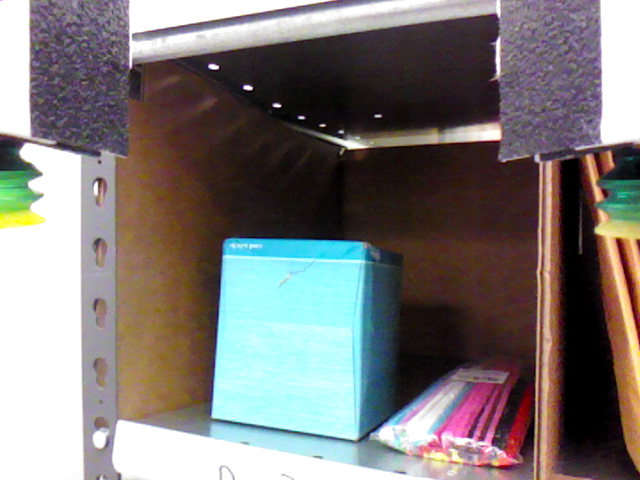
\includegraphics[width=3.5cm]{apc_color1}}
  \hskip0.2cm
  \subfloat{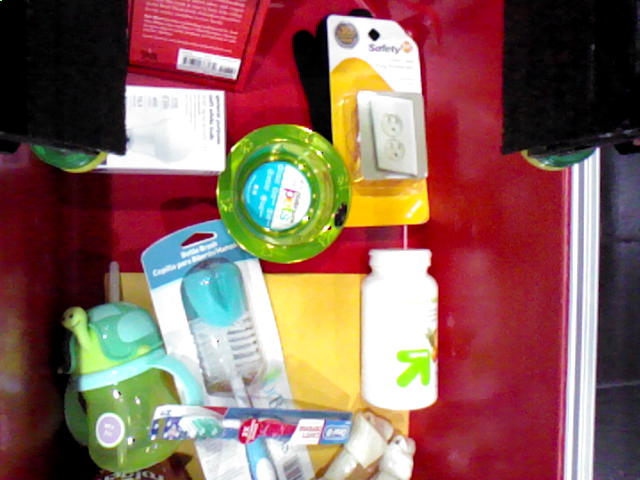
\includegraphics[width=3.5cm]{apc_color2}}
  \hskip0.2cm
  \subfloat{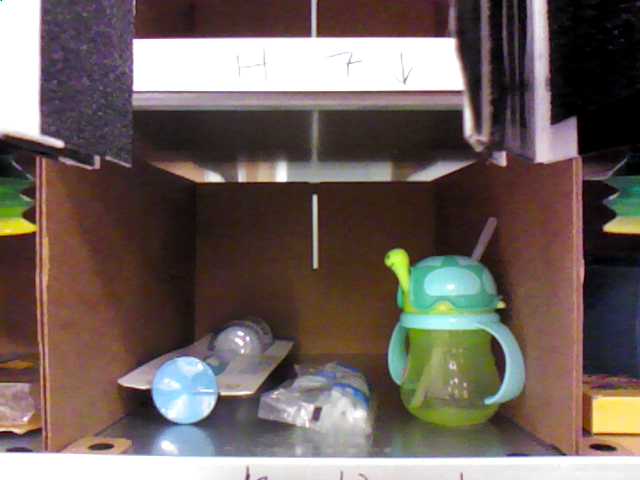
\includegraphics[width=3.5cm]{apc_color3}}
  \hskip0.2cm
  \subfloat{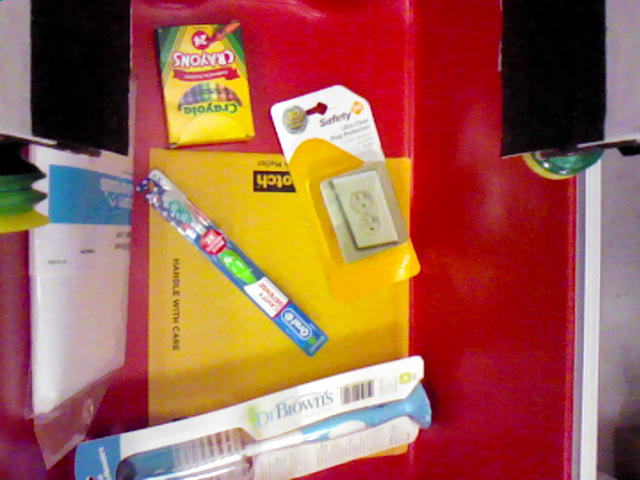
\includegraphics[width=3.5cm]{apc_color4}}
  \vfill
  \subfloat{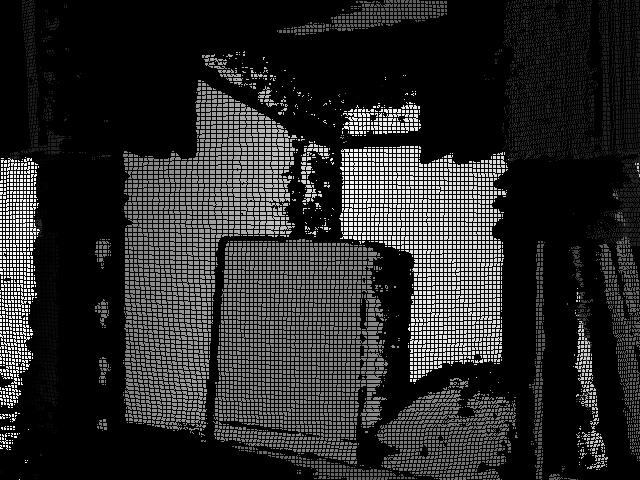
\includegraphics[width=3.5cm]{apc_depth1}}
  \hskip0.2cm
  \subfloat{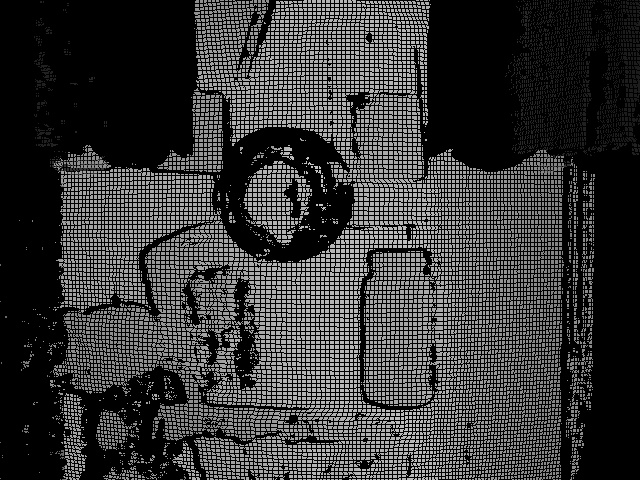
\includegraphics[width=3.5cm]{apc_depth2}}
  \hskip0.2cm
  \subfloat{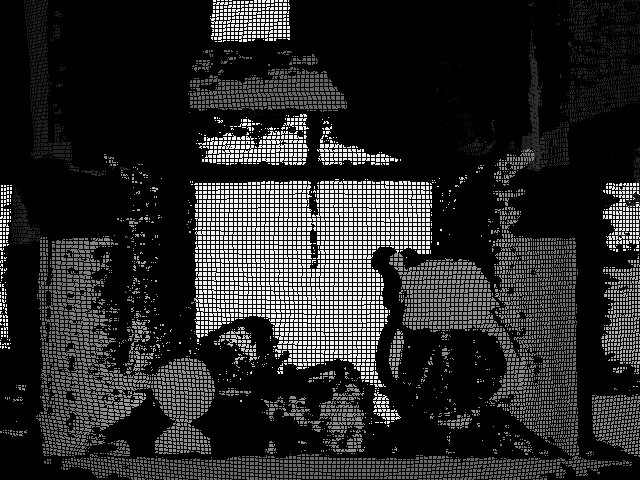
\includegraphics[width=3.5cm]{apc_depth3}}
  \hskip0.2cm
  \subfloat{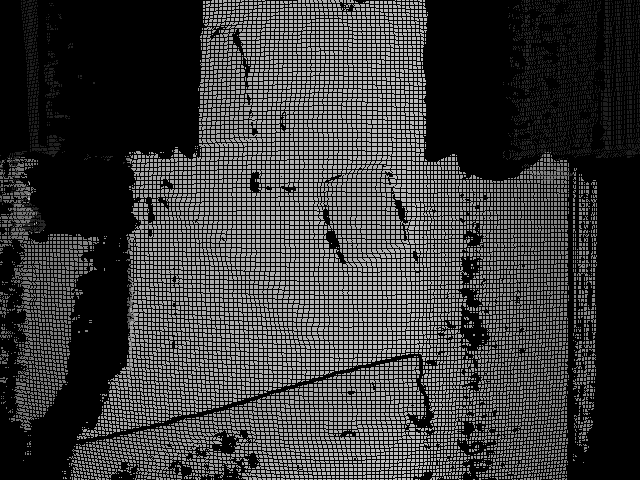
\includegraphics[width=3.5cm]{apc_depth4}}
  \caption{APC数据集部分数据:第一栏为彩色图像,第二栏为与彩色图像相匹配的深度图}
  \label{fig:apc_dataset}
\end{figure}

APC数据集中标注的标签可以认为是每个物体在相机坐标系下的位姿和类别,对于设计的算法来说需要的是物体的类别(Class)、边界框(Bounding Box)和掩模(Mask),因此需要对原始标注数据进行一些处理,因为APC还提供了每类物体的CAD模型,并且相机的内参矩阵也在数据集中提供了,因此可以将CAD模型转换为点云后齐次变换到所标注的对应物体在相机坐标系下的位姿,然后利用相机内参矩阵将物体点云投影到图像平面,从而获得物体的Mask,进而可以得到物体的Bounding Box。需要注意的是由于一个场景中有多个物体,在不同相机位姿下会出现遮挡,因此需要对被遮挡物体的Mask进行相应的裁剪,对于几乎被完全遮挡的物体可以去除掉,判断物体是否遮挡可以通过物体点云距离相机原点的距离远近判断。将一张图中物体位姿得到Mask和Boudning Box的处理流程如下所示:
\begin{enumerate}
\item 对于图中标注的每个物体:
  \begin{itemize}
  \item 将对应物体的3D点云变换到物体标注的位姿
  \item 根据相机内参矩阵将3D点云投影到图像平面,获得物体的Mask以及Mask对应的深度图Depth
  \end{itemize}
\item 遍历像素索引i:
  \begin{itemize}
  \item 如果在索引i出存在多张Mask的值有效,保留Depth值最小的Mask,将其余Mask在索引i处置为无效
  \end{itemize}
\item 对于每个物体的Mask:
  \begin{itemize}
  \item 如果Mask中有效像素点小于阈值$T$,删除该Mask
  \item 根据mask有效像素点的坐标计算对应的Bounding Box
  \end{itemize}
\end{enumerate}
处理后的部分图片的ground truth(Class,Mask,Boudning Box)如图\ref{fig:apc_gt}所示。
\begin{figure}[ht]
  \centering
  \subfloat{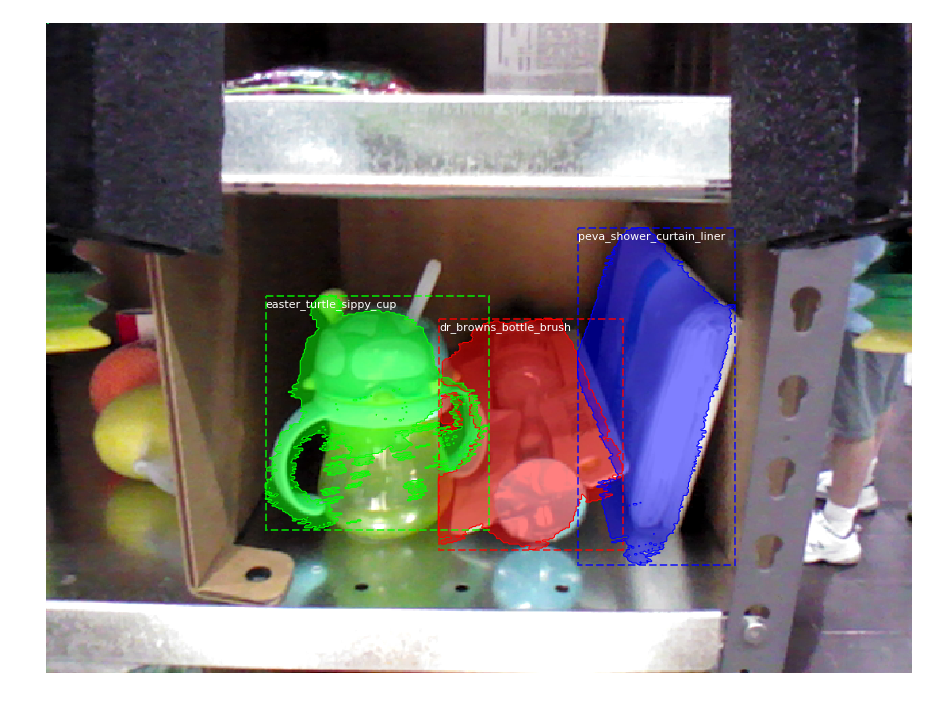
\includegraphics[width=6cm]{apc_gt1}}
  \hskip1cm
  \subfloat{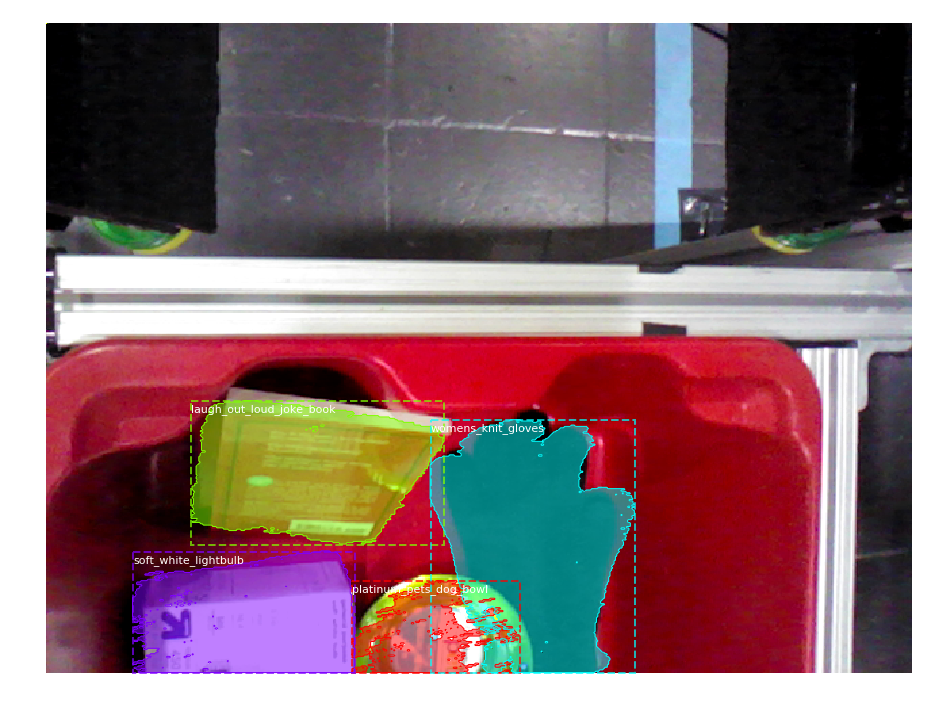
\includegraphics[width=6cm]{apc_gt2}}
  \vfill
  \subfloat{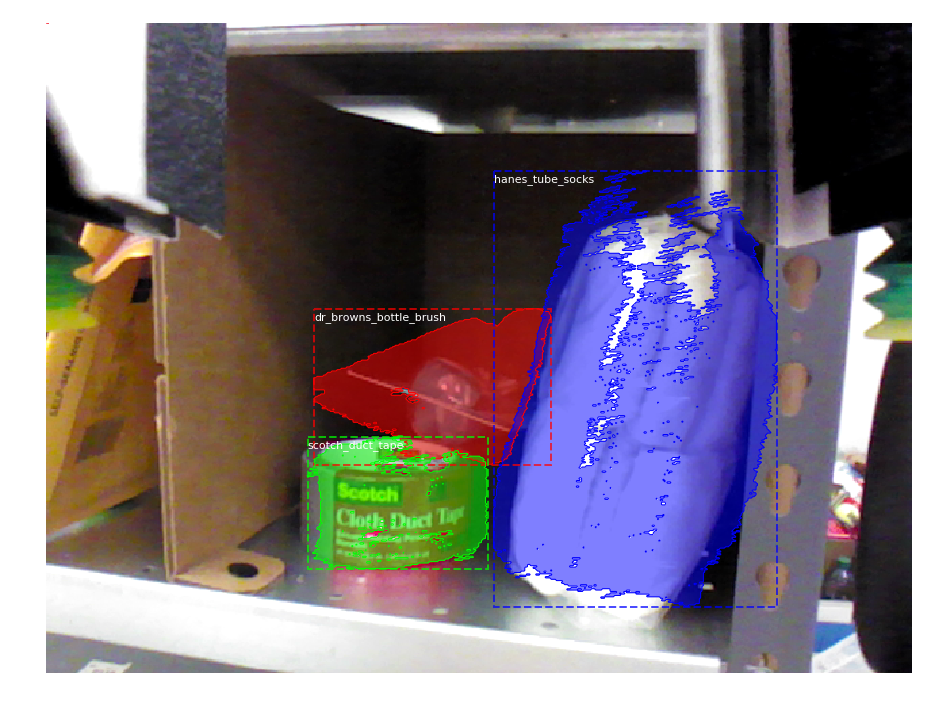
\includegraphics[width=6cm]{apc_gt3}}
  \hskip1cm
  \subfloat{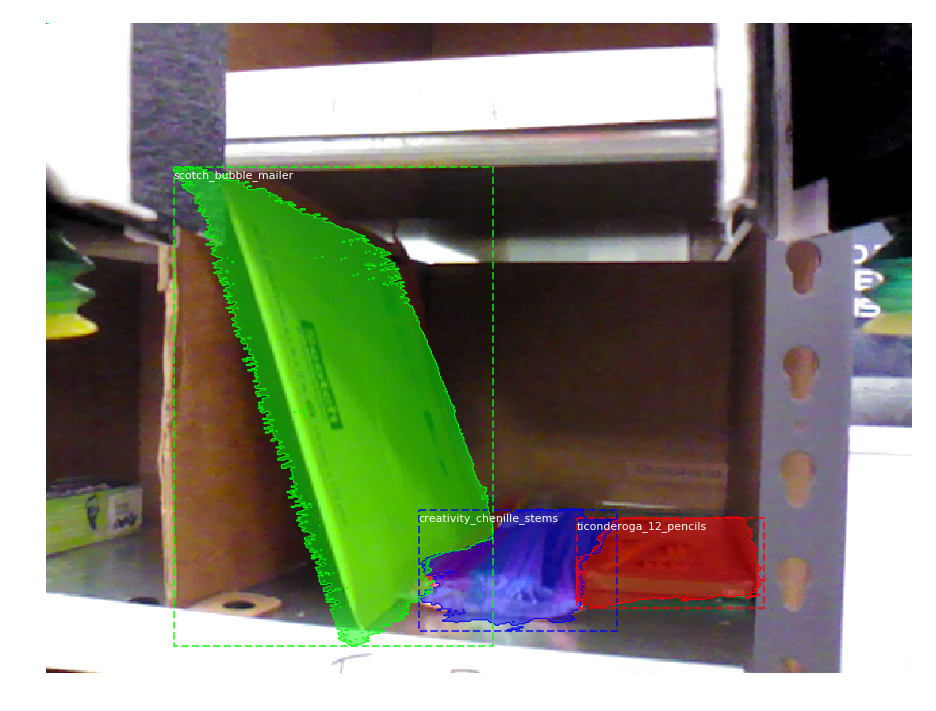
\includegraphics[width=6cm]{apc_gt4}}
  \caption{APC数据集部分标注数据}
  \label{fig:apc_gt}
\end{figure}
从图\ref{fig:apc_gt}可以看出处理后的Mask基本覆盖了物体,Boudning Box也正确框出了物体,唯一的缺点是所生成的Mask有时候有些缺失,没有人工标注的完美,如图\ref{fig:apc_gt}中第一张图中的瓶子(easter turtle sippy cup)标注的Mask有很多缺失,根本原因是所使用的物体的CAD模型是通过相机采集生成的,其转换的3D点云质量并不是十分理想,其3D点云比较稀疏并且有部分缺失,如图\ref{fig:apc_model}所示,这个瓶子的点云有严重的缺失,主要原因是瓶子透明,所以相机难以采集其深度信息。
\begin{figure}[ht]
  \centering
  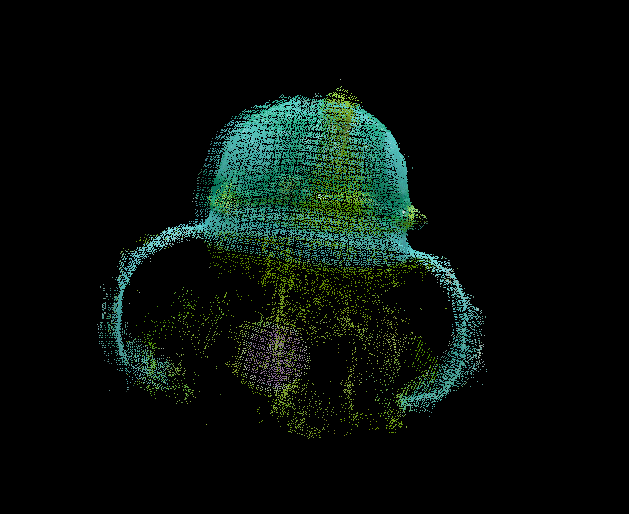
\includegraphics[width=10cm]{apc_model1}
  \caption{easter turtle sippy cup point cloud}
  \label{fig:apc_model}
\end{figure}
模型点云的缺失,因此将点云投影到图像平面生成的mask也有部分缺失,尽管已经对生成的mask进行了一些滤波处理,但部分Mask还是有明显的缺失。

总体来说,尽管生成的ground truth的质量没有人工标注的ground truth质量好,但对本实验来说已经够用,并且相比人工标注这种半自动化的标注方式节省了大量时间和金钱成本。

workpiece数据集有三类物体,共2k组图片。该数据集与APC数据集最大的不同是,同一张图片中存在大量不同位姿的同种物体,并且三类物体都缺少纹理(textureless),因此Faster R-CNN和Mask R-CNN在该数据集上的表现理论上应该大大不如所设计的检测模块。部分数据集中的图片如图\ref{fig:wp_dataset}所示。
\begin{figure}[ht]
  \centering
  \subfloat{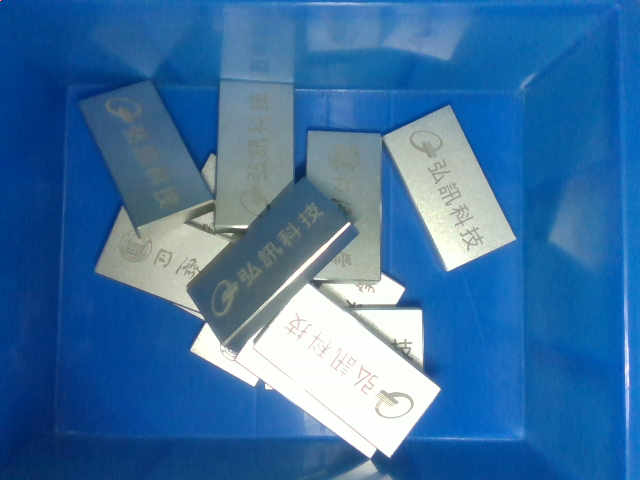
\includegraphics[width=3.5cm]{wp_color1}}
  \hskip0.2cm
  \subfloat{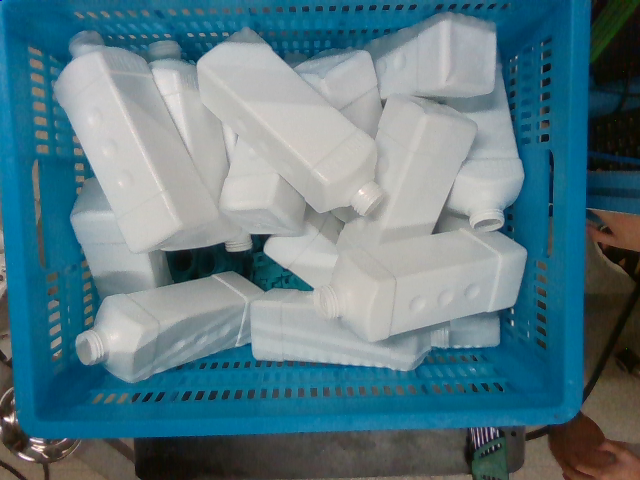
\includegraphics[width=3.5cm]{wp_color2}}
  \hskip0.2cm
  \subfloat{\includegraphics[width=3.5cm]{wp_color3}}
  \vfill
  \subfloat{\includegraphics[width=3.5cm]{wp_depth1}}
  \hskip0.2cm
  \subfloat{\includegraphics[width=3.5cm]{wp_depth2}}
  \hskip0.2cm
  \subfloat{\includegraphics[width=3.5cm]{wp_depth3}}
  \caption{workpiece数据集部分图片}
  \label{fig:wp_dataset}
\end{figure}
workpiece数据集的ground truth由人工标定,其中据测试集中有的ground truth不仅包括了物体的Class,Mask,Bounding box,还有物体的位姿,并且由于三类物体都是工厂中的工件,因此也提供三类物体精确的CAD模型。

{\kai 算法实现}主要通过Tensorflow框架使用python语言实现,详细代码见Github项目地址\footnote{\url{https://github.com/freealong/Mask\_RCNN}}。

{\kai 评价的指标}主要是检测的精确度AP(Average Precision)以及算法的时间性能FPS。FPS是每秒能检测的图片数比较好理解,AP是BBox或者Mask交并比的精确度。具体地,如图\ref{fig:iou}所示,
\begin{figure}[ht]
  \centering
  \includegraphics[width=8cm]{iou}
  \caption{bounding box交并比}
  \label{fig:iou}
\end{figure}
两个BBox的交并比定义为:
\begin{equation}
  IoU = \frac{S_1\cap S_2}{S_1\cup S_2}
\end{equation}
$AP_{0.5}$表示检测的结果与ground truth的交并比大于0.5的个数占总体检测个数的比例,显然定义精度的$IoU$大小会影响最终评价的质量,过小和过大的最小$IoU$都不能很好地反应算法的精缺度,因此将评价的主要精确度定义如下:
\begin{equation}
  AP = \frac{1}{10}\sum_{i=0}^{9}{AP_{0.5 + 0.5i}}
\end{equation}
检测结果换为Mask精确度的定义也类似,只需用Mask的交并比代替BBox的交并比。

{\kai 模型训练}在实验室的服务器上进行,服务器有两块Intel(R) Xeon(R) E5-2683 v3(2.00GHz)的CPU,4块TITAN X GPU。模型训练时为了减少训练时间,4块GPU都使用了。在APC数据集上,训练用了约6k组图片,剩下的1k多组图片用于测试,基于Faster R-CNN的检测模块训练用了40个小时左右,基于Mask R-CNN的检测模块用了48个小时左右;在workpiece数据集上,训练用了约1.6k组图片,剩下的400组图片用于测试,基于Faster R-CNN的检测模块训练用了30个小时左右,基于Mask R-CNN的检测模块用了36小时左右。

{\kai 实验结果}:
在APC数据集上,本文的检测模块与原始的Faster R-CNN和Mask R-CNN的精确度如表\ref{tab:ap1}所示,在测试集上的部分图片检测结果见图\ref{fig:apc_res}。
\begin{table}[ht]
  \centering
  \caption{APC数据集上的精确度}
    \begin{tabular}{cccccc}
      \toprule
      &input&output&$AP$&$AP_{0.5}$&$AP_{0.75}$ \\
      \midrule
      Faster R-CNN&RGB&bbox&33.26&56.29&34.03 \\
      \bf{Our method(based on Faster R-CNN)}&RGB+HHA&bbox&\bf{34.55}&\bf{57.99}&\bf{34.69} \\
      Mask R-CNN&RGB&mask&32.34&55.78&33.12 \\
      \bf{Our method(based on Mask R-CNN)}&RGB+HHA&mask&\bf{33.94}&\bf{56.45}&\bf{33.99} \\
      \bottomrule
    \end{tabular}
  \label{tab:ap1}
\end{table}
\begin{figure}[ht]
  \centering
  \subfloat{\includegraphics[width=4.5cm]{detect_apc_res1}}
  \hskip2pt
  \subfloat{\includegraphics[width=4.5cm]{detect_apc_res2}}
  \hskip2pt
  \subfloat{\includegraphics[width=4.5cm]{detect_apc_res3}}
  \caption{APC数据集上部分检测结果}
  \label{fig:apc_res}
\end{figure}
从表\ref{tab:ap1}中可以看出在APC数据集上本文基于Faster R-CNN所提出的方法相比Faster R-CNN的精确度提高了1.3个百分点左右,基于Mask R-CNN所提出的方法相比Mask R-CNN提高了0.8个百分点左右。整体来说对精确度的提高并不是十分明显,究其原因,从图\ref{fig:apc_dataset}可以看到APC数据集中的物体大多也是纹理丰富的,单从RGB图就可以训练出一个很好的模型,因此增加HHA通道,对模型精确度的提升十分有限,反而降低了算法的FPS。

在workpiece数据集上的检测精确度如表\ref{tab:ap2}所示,在测试集上的部分图片检测结果见图\ref{fig:wp_res}。
\begin{table}[ht]
  \centering
  \caption{workpiece数据集上的精确度}
    \begin{tabular}{cccccc}
      \toprule
      &input&output&$AP$&$AP_{0.5}$&$AP_{0.75}$ \\
      \midrule
      Faster R-CNN&RGB&bbox&18.78&37.49&19.46 \\
      \bf{Our method(based on Faster R-CNN)}&RGB+HHA&bbox&\bf{32.39}&\bf{56.37}&\bf{33.54} \\
      Mask R-CNN&RGB&mask&16.12&35.95&18.74 \\
      \bf{Our method(based on Mask R-CNN)}&RGB+HHA&mask&\bf{30.98}&\bf{53.74}&\bf{32.19} \\
      \bottomrule
    \end{tabular}
  \label{tab:ap2}
\end{table}
\begin{figure}[ht]
  \centering
  \subfloat{\includegraphics[width=4.5cm]{detect_wp_res1}}
  \hskip0.2cm
  \subfloat{\includegraphics[width=4.5cm]{detect_wp_res2}}
  \hskip0.2cm
  \subfloat{\includegraphics[width=4.5cm]{detect_wp_res3}}
  \caption{workpiece数据集上部分检测结果}
  \label{fig:wp_res}
\end{figure}
从表\ref{tab:ap2}可以看出在workpiece数据集上,本文基于Faster R-CNN所提出的检测模块相比Faster R-CNN的精确度提高了13.6个百分点左右,基于Mask R-CNN所提出的检测模块相比Mask R-CNN提高了约14.8个百分点。显然,本文所提出的检测模块在workpiece数据集上精确度相比原算法有了大大的提高,从图\ref{fig:wp_dataset}可以发现workpiece数据集中的图片包含的都是一些缺少纹理的物体,并且有大量同种物体混杂在一起,有时候人眼也很难从中区分单个目标,因此可能单从RGB图难以训练出一个准确率较高的模型来检测目标。而这些缺少纹理的大量物体在深度图,尤其是变换后的HHA图上十分容易区分出来,因此引入HHA后,增加了更多信息,最终训练得到的模型的准确度相比原算法有了巨大的提升。

所提出的检测模块的时间性能见表\ref{tab:fps},
由于两个数据集内图片的大小都是一样的,因此算法的时间性能在两个数据集上并不会有什么差异,因此表\ref{tab:fps}中直接统计了算法在两个数据集测试样本上FPS的平均值。从表\ref{tab:fps}可以看出本文所提出的检测模块与Faster R-CNN和Mask R-CNN相比,普遍具有更低的FPS,主要因为增加了HHA数据并且增加了STN模块。但考虑到本文算法的具体应用,适当降低的FPS并不会对具体使用造成什么影响。
\begin{table}[ht]
  \centering
  \caption{算法时间性能}
  \begin{tabular}{cc}
    \toprule
    &FPS \\
    \midrule
    Faster R-CNN&5.5 \\
    \bf{Our method(based on Faster R-CNN)}&\bf{3.2} \\
    Mask R-CNN&4.1 \\
    \bf{Our method(based on Mask R-CNN)}&\bf{2.5} \\
    \bottomrule
  \end{tabular}
  \label{tab:fps}
\end{table}

\section{匹配模块}
\label{sec:matcher}

\subsection{模块框架设计}
本文设计的匹配模块的框图如图\ref{fig:4pcs-pe}所示,
\begin{figure}[ht]
  \centering
  \includegraphics[width=12cm]{4pcs-pe}
  \caption{匹配模块框架}
  \label{fig:4pcs-pe}
\end{figure}
匹配模块的输入是两个点云(点集)\footnote{本文对点集(point set)与点云(point cloud)不做区分,都指包含坐标点的集合}$P$和$Q$,输出的是这两个点云之间的刚体变换$T$。

点云之间的匹配问题并不是一个新的问题,解决该问题的算法也有很多,尤其是近些年来,随着几何扫描相关技术的发展,如何将多次扫描或者多个设备采集的三维信息统一到一个坐标系下成为研究的热点,这些问题也是计算机几何学和计算机视觉中的基础问题。

其中一个比较流行的算法是通过使用稳定的局部几何描述子来匹配得到粗略的刚体变换,然后紧接着使用ICP算法\cite{besl1992method}迭代获取较为精确的刚体变换\cite{li2005multiscale}。这种算法的效果十分取决于所选取的描述子,通常一般的描述子对传感器噪声都比较敏感,尤其是一些低精度的传感器,常用的局部几何特征描述子有SHOT\cite{salti2014shot}、FFPH\cite{rusu2009fast}等;还有一种比较流行的方法是通过几何希哈方法从事先设置好的候选集中来选择合适的刚体变换\cite{wolfson1997geometric};一些随机算法,如RANSAC(Random Sample Consesue)\cite{bolles1981ransac}通常需要足够长的时间才能保证得到合适的解。

上述介绍的一些算法,有些对噪声的鲁棒性不强,有些时间复杂度极高,有些也难以处理部分重叠的情况,即点集$P$和$Q$之间只有一部分点集是相匹配的,因此难以实际直接应用到本文所需要解决的问题,其效果也难以让人满意。对此,本文基于4PCS(4-Points Congruent Sets)\cite{aiger20084}算法设计了有效解决点云匹配的匹配模块。

所设计的匹配模块首先针对4PCS算法的不足,对其进行改进,然后通过对离群点进行过滤和利用ICP算法进行迭代提升最终匹配的精度。从图\ref{fig:4pcs-pe}中可以看出所设计的匹配模块主要由三个部分组成:改进的4PCS算法(Angle-fixed 4PCS)、Outlier filter和ICP算法。改进的4PCS算法根据输入的两个点云输出两个点集之间的粗略的变换关系;Outlier filter根据改进的4PCS算法的输出对点集$P'$和$Q'$进行滤波,去掉一些离群点,用以提高下一步ICP算法的精度;ICP模块通过以改进后的4PCS算法输出的变换关系为初始值对滤波后的两个点集进行迭代求解最佳的刚体变换关系,输出最终的变换关系$T$和匹配的分数$S$,$T$也是目标的位姿,$S$是点云匹配误差的倒数,\ref{sec:matcher_exp}小节会具体介绍匹配误差。

\subsection{4PCS算法的改进}
介绍改进的4PCS算法之前,首先必须详细介绍一下4PCS算法。4PCS算法是用于求解LCP(Largest Common Pointset)问题的一个算法,LCP问题的定义如下:

{\kai LCP问题:给定两个点集$P$和$Q$,在给定距离误差$\delta$下,求解点集$P$的最大子集$P'$,使得$T(P')$和点集$Q$之间的距离在合适的距离度量下小于$\delta$,其中$T$是一个刚体变换。}

\begin{algorithm}
  \caption{4PCS算法}
  \label{alg:4pcs}
  \KwIn{Point sets $P$ and $Q$, measure level $\delta$}
  \KwOut{Rigid transform $T$}
  $h\leftarrow 0$\;
  \For {$i = 1$ to $L$} {
    $B\leftarrow$ SELECTCOPLANARBASE($P$)\;
    $U\leftarrow$ FINDCONGRUENT($B,Q,\delta$)\;
    \ForAll {4-points coplannar sets $U_i\in U$} {
      $T_i\leftarrow$ best rigid transform that aligns $B$ to $U_i$ in the least square sense\;
      Find $S_i\subseteq P$, such that $d(T_i(S_i), Q)\leq\delta$\;
    }
    $k\leftarrow arg\;\underset{i}{max}\left\{|S_i|\right\}$\;
    \If {$|S_k| > h$} {
      $h\leftarrow |S_k|$\;
      $T\leftarrow T_k$\;
    }
    \Return $T$\;
  }
  \BlankLine
  \BlankLine
  \BlankLine
  \BlankLine
  \SetKwProg{Def}{def}{:}{}
  \Def{FINDCONGRUENT($B:=\left\{\mathbf{b}_1,\mathbf{b}_2,\mathbf{b}_3,\mathbf{b}_4\right\},Q,\delta)$} {
    $d_1\leftarrow\;\parallel\mathbf{b}_1-\mathbf{b}_2\parallel$\;
    $d_2\leftarrow\;\parallel\mathbf{b}_3-\mathbf{b}_4\parallel$\;
    计算$R_1\equiv\left\{(\mathbf{p}_i,\mathbf{p}_j)\;|\;\mathbf{p}_i,\mathbf{p}_j\;\in Q\right\}$,使得$\parallel\mathbf{p}_i-\mathbf{p}_j\parallel\;\in [d_1-\delta,d_1+\delta]$\;
    计算$R_2\equiv\left\{(\mathbf{p}_i,\mathbf{p}_j)\;|\;\mathbf{p}_i,\mathbf{p}_j\;\in Q\right\}$,使得$\parallel\mathbf{p}_i-\mathbf{p}_j\parallel\;\in [d_2-\delta,d_2+\delta]$\;
    \ForAll {$r_{1i}\in R_1$} {
      计算与定量$r_1$和$r_2$相关的四个点$\left\{\mathbf{e}_{1i}^1,\mathbf{e}_{1i}^2,\mathbf{e}_{1i}^3,\mathbf{e}_{1i}^4\right\}$,记$\Pi(\mathbf{e}_{1i}^j)=r_{1i}$\;
    }
    对点集$\left\{\mathbf{e}_{1i}^j\right\}$在$\mathbb{R}^3$空间建立range tree的数据结构\;
    \ForAll {$r_{2i}\in R_1$} {
      计算与定量$r_1$和$r_2$相关的四个点$\left\{\mathbf{e}_{2i}^1,\mathbf{e}_{2i}^2,\mathbf{e}_{2i}^3,\mathbf{e}_{2i}^4\right\}$,记$\Pi(\mathbf{e}_{1i}^j)=r_{1i}$\;
    }
    $U'\leftarrow\varnothing$\;
    \ForAll {$\mathbf{e}_{2i}^j$} {
      在range tree中以$\delta$为领域检索点$\mathbf{e}_{2i}^j$附近的点,对于每个检索到的点$\mathbf{q}$,建立与$B$相对应的4个点的点集$U'\leftarrow\left\{U',(\Pi(\mathbf{q}),\Pi(\mathbf{e}_{2i}^j))\right\}$\;
    }
    \Return $U'$\;
  }
\end{algorithm}

4PCS算法具体的流程如\ref{alg:4pcs}所示,该算法输入两个点集$P$和$Q$,还有距离参数$\delta$,返回两个点集之间的刚体变换$T$。4PCS基于以下事实:{\kai 共面点集中定义的比例在仿射变换,包括刚体运动中保持不变。}举例来说,定义点集$X:=\left\{\mathbf{a},\mathbf{b},\mathbf{c},\mathbf{d}\right\}$,其中4个点不都在同一条直线上,设直线$ab$和$cd$相交于点$\mathbf{e}$,定义两个比例:
\begin{equation}
  \begin{array}{ccc}
    r_1& =& {\parallel \mathbf{a}-\mathbf{e}\parallel}/{\parallel \mathbf{a}-\mathbf{b}\parallel}\\
    r_2& =& {\parallel \mathbf{c}-\mathbf{e}\parallel}/{\parallel \mathbf{c}-\mathbf{d}\parallel}
  \end{array}
\end{equation}
则在仿射变换下所定义的$r_1$和$r_2$均保持不变,如图\ref{fig:4points}。
\begin{figure}[ht]
  \centering
  \includegraphics[width=12cm]{4points}
  \caption{4-points比例的仿射不变性}
  \label{fig:4points}
\end{figure}
如果曲面$S_1$和$S_2$匹配,并且4-points共面基在重叠区域,则$\mathbf{a},\mathbf{b},\mathbf{c},\mathbf{d}$对应的四个点$\mathbf{a}',\mathbf{b}',\mathbf{c}',\mathbf{d}'$也共面,并且
\begin{equation}
  \begin{array}{ccc}
    {\parallel \mathbf{a}'-\mathbf{e}'\parallel}/{\parallel \mathbf{a}'-\mathbf{b}'\parallel}&=&r_1\\
    {\parallel \mathbf{c}'-\mathbf{e}'\parallel}/{\parallel \mathbf{c}'-\mathbf{d}'\parallel}&=&r_2\\
  \end{array}
\end{equation}


4PCS算法另一个关键技术是使用了{\kai 宽基}(\emph{wide-base}),相比于一般的基,宽基中基的长度更长,如图\ref{fig:wide-base}所示,图片上半部分是使用宽基匹配的曲线,图片下半部分是使用一般的基匹配的曲线,显然,通过比较可以发现宽基相比普通基有更稳定的匹配结果,相关理论证明见文献\cite{goodrich1994practical}。
\begin{figure}[ht]
  \centering
  \includegraphics[width=14cm]{wide-base}
  \caption{宽基的匹配稳定性}
  \label{fig:wide-base}
\end{figure}

回到4PCS算法具体实现,算法的主体其实是一个RANSAC循环,每次循环首先会从点集$P$中挑选共面的宽基$B$,具体实现时,先从点集$P$中随机选取3个点,然后在剩下的点中选取第四个点构成共面的四点,第四个点的选取尽可能使得每个点之间的距离最大(因为我们要使用宽基),并且与前3个点近似共面(显然由于噪声的存在,完全共面并不现实),但如果第四个点选取的过远也会出现问题,因为如果宽基超过两个点集的重叠区域则难以匹配,因此当选以最大距离取宽基造成误差变大时以$f=1,0.5,0.25,\ldots$的比率降低最大距离来选取宽基。

在点集$P$中选取好宽基$B$后,算法下一步会在点集$Q$中通过4-points的仿射不变性找出所有与宽基$B$“全等”的基,构成集合$U$。在$Q$中选取基的方法见算法\ref{alg:4pcs}中的FINDCONGRUENT函数,函数首先使用基$B$中的点先定义两个仿射无关的比例,如图\ref{fig:findbase}中左边的图所示。
\begin{figure}[ht]
  \centering
  \includegraphics[width=15cm]{findbase}
  \caption{寻找近似“全等”的基示意图}
  \label{fig:findbase}
\end{figure}
假设在点集$Q$中找到两点$\mathbf{q}_1$和$\mathbf{q}_2$,并且$\left|\parallel \mathbf{q}_1-\mathbf{q}_2\parallel - \parallel \mathbf{a}-\mathbf{b}\parallel\right| \leq \delta$,则点$\mathbf{q}_1,\mathbf{q}_2$有可能与点$\mathbf{a}, \mathbf{b}$对应,则直线$\mathbf{a}\mathbf{b}$与$\mathbf{c}\mathbf{d}$相交的点$\mathbf{e}$的对应点可能为
\begin{equation}
  \mathbf{e}_1 = \mathbf{q}_1 + r1(\mathbf{q}_2-\mathbf{q}_1)
\end{equation}
或者
\begin{equation}
  \mathbf{e}_1 = \mathbf{q}_2 + r1(\mathbf{q}_1-\mathbf{q}_2)
\end{equation}
同理也可以根据$\mathbf{c},\mathbf{d}$的对应点(设为$\mathbf{q}_3, \mathbf{q}_4$)求得$\mathbf{e}$的对应点
\begin{equation}
  \mathbf{e}_2 = \mathbf{q}_3 + r1(\mathbf{q}_4-\mathbf{q}_3)
\end{equation}
或者
\begin{equation}
  \mathbf{e}_2 = \mathbf{q}_4 + r1(\mathbf{q}_3-\mathbf{q}_4)
\end{equation}
则当$\mathbf{e}_1\approx \mathbf{e}_2$时,$\mathbf{q}_1,\mathbf{q}_2,\mathbf{q}_3,\mathbf{q}_4$就是我们所要找的一组与点$\mathbf{a},\mathbf{b},\mathbf{c},\mathbf{d}$近似“全等”的基,如图\ref{fig:findbase}中右边图中的$\mathbf{q}_5,\mathbf{q}_3,\mathbf{q}_4,\mathbf{q}_1$。

具体实现时,当我们在点集$Q$中找出了所有可能的$\mathbf{e}_1$和$\mathbf{e}_2$后,找出其中近似相等的$\mathbf{e}_1$和$\mathbf{e}_2$可以通过range树\cite{arya1998optimal}来实现,对于大小为$n$的点集,range树的建立时间复杂度为$O(n\lg n)$,查询附近点的时间复杂度为$O(\lg n + k)$,其中$k$是查询到点的个数。

在$Q$中找出所有与基$B$近似“全等”的基后,下一步就是计算出最优的刚体变换$T$。对于$U$中的每个基$U_i$,我们可以利用最小二乘\cite{horn1987closed}的思想计算$B$到$U_i$的刚体变换$T_i$。得到刚体变换$T_i$后,我们将点集$P$进行变换$T_i$,然后对变换后的点集中的点在$Q$中查找最近点,统计最近点距离小于$\delta$的个数$S_i$,$S_i$也是评价$T_i$效果的分数,分数越高的$T_i$就是我们要求的最优刚体变换$T$。

仔细研究4PCS算法,可以发现从点集$Q$中提取的基与$B$并不是全等的,如图\ref{fig:4pcs-flaw}所示,
\begin{figure}[ht]
  \centering
  \includegraphics[width=12cm]{4pcs-flaw}
  \caption{4PCS中"全等“的基}
  \label{fig:4pcs-flaw}
\end{figure}
将线段$\mathbf{q}_1\mathbf{q}_2$绕交点转动一定角度后便不再与原基全等,但是4PCS仍然会找出点$\mathbf{q}_1',\mathbf{q}_2',\mathbf{q}_3,\mathbf{q}_4$作为与$\mathbf{p}_1',\mathbf{p}_2',\mathbf{p}_3,\mathbf{p}_4$全等的基。这一缺点会导致4PCS算法需要更多的求解时间,并且还有可能影响最终的匹配结果。因此,对4PCS改进去除这些与原基不是全等的基很有必要。改进后的算法如算法\ref{alg:a4pcs}所示,与原算法的区别在于,在FINDCONGRUENT函数后面增加了滤去不全等的基的步骤FILTERCONGRUENT函数。FINDCONGRUENT函数输入原基$B$、在$Q$中找到的与$B$全等的基的集合,以及允许的角度阈值$\epsilon$,然后通过比较基中两个向量之间的点积来判断角度是否近似相等,但由于我们无法确定向量的方向,即无法确定点$\mathbf{b}_1$是与$\mathbf{q}_1$对应还是与$\mathbf{q}_2$对应,因此$U$中基的两个向量之间的角度可能与$B$中相差180度。
\begin{algorithm}
  \caption{改进的4PCS算法}
  \label{alg:a4pcs}
  \KwIn{Point sets $P$ and $Q$, distance tolerance $\delta$, angle tolerance $\epsilon$}
  \KwOut{Rigid transform $T$}
  $h\leftarrow 0$\;
  \For {$i = 1$ to $L$} {
    $B\leftarrow$ SELECTCOPLANARBASE($P$)\;
    $U\leftarrow$ FINDCONGRUENT($B,Q,\delta$)\;
    $U\leftarrow$ FILTERCONGRUENT($B,U,\epsilon$)\;
    \ForAll {4-points coplannar sets $U_i\in U$} {
      $T_i\leftarrow$ best rigid transform that aligns $B$ to $U_i$ in the least square sense\;
      Find $S_i\subseteq P$, such that $d(T_i(S_i), Q)\leq\delta$\;
    }
    $k\leftarrow arg\;\underset{i}{max}\left\{|S_i|\right\}$\;
    \If {$|S_k| > h$} {
      $h\leftarrow |S_k|$\;
      $T\leftarrow T_k$\;
    }
    \Return $T$\;
  }
  \BlankLine
  \BlankLine
  \BlankLine
  \BlankLine
  \SetKwProg{Def}{def}{:}{}
  \Def{FILTERCONGRUENT($B:=\left\{\mathbf{b}_1,\mathbf{b}_2,\mathbf{b}_3,\mathbf{b}_4\right\},U,\epsilon)$} {
    $U'\leftarrow \varnothing$\;
    $a\leftarrow \overrightarrow{\mathbf{b}_1\mathbf{b}_2}\cdot \overrightarrow{\mathbf{b}_3\mathbf{b}_4}$\;
    \ForAll {$U_i:=\left\{\mathbf{q}_1,\mathbf{q}_2,\mathbf{q}_3,\mathbf{q}_4\right\}\in U$} {
      $a'\leftarrow \overrightarrow{\mathbf{q}_1\mathbf{q}_2}\cdot \overrightarrow{\mathbf{q}_3\mathbf{q}_4}$\;
      \If {$a'\in [a-\epsilon,a+\epsilon]\cup [-a-\epsilon,-a+\epsilon]$} {
        $U'\leftarrow \left\{U',U_i\right\}$\;
      }
    }
    \Return $U'$\;
  }
\end{algorithm}

\subsection{匹配精度优化}
实验表明,经过改进的4PCS算法输出的刚体变换$T$的精度不高,所以,所设计的匹配模块在改进的4PCS算法后面通过滤波和迭代来提升最终匹配的精度。

实际要匹配的两个点云往往不是完全重合的,也就是说两个点云匹配的时候有许多离群点,尤其是目标点云由BBox分割得到的情况,如图\ref{fig:outlier-pointcloud}所示,
\begin{figure}[ht]
  \centering
  \subfloat[目标3D模型转化的点云]{
    \includegraphics[width=6cm]{object-cloud}
  }
  \hskip1cm
  \subfloat[由BBox分割得到的点云]{
    \includegraphics[width=6cm]{target-cloud}
  }
  \caption{实际要匹配的两个点云}
  \label{fig:outlier-pointcloud}
\end{figure}
由BBox分割得到的点云由许多点并不与目标3D模型相匹配,将这些离群点滤去有助于提高最终的匹配精度,因此本文设计了Outlier filter模块用于滤去这些离群点,具体的算法如\ref{alg:outlier-filter}所示。
\begin{algorithm}[ht]
  \caption{Outlier filter算法}
  \label{alg:outlier-filter}
  \KwIn{Point sets $P$ and $Q$, Initial transform $T$, Distance tolerance $\delta$}
  \KwOut{Point sets $P'$ and $Q'$}
  $P'\leftarrow P$\;
  $Q'\leftarrow \varnothing$\;
  \ForAll {point $\mathbf{p}_i\in P$} {
    $\mathbf{p}_i\leftarrow T(\mathbf{p}_i)$\;
  }
  对点集$P$在$\mathbb{R}^3$空间建立kd树的数据结构\;
  \ForAll {point $\mathbf{q}_i\in Q$} {
    在kd树中检索出距离点$\mathbf{q}_i$最近的点$\mathbf{p}$\;
    $d\leftarrow\;\parallel\mathbf{q}_i-\mathbf{p}\parallel$\;
    \If {$d \leq \delta$} {
      $Q'\leftarrow \left\{Q', \mathbf{q}_i\right\}$\;
    }
  }
  \Return $P'$,$Q'$\;
\end{algorithm}
算法输入点集$P$和$Q$,需要参数初始刚体变换$T$,以及允许的距离误差$\delta$,由于点集$P$是由物体的CAD模型转换过来的,因此不对其进行滤波,只对点集$Q$进行离群点去除。具体方法是,首先使用$T$对点集$P$进行刚体变换;然后对变换后的点集建立kd树,建立kd树的目的是为了快速在点集$P$中找到距离某点最近的点,其查找的时间复杂度为$O(kN^{1-1/k})$,其中$k$是所建立kd树的维数,显然对于三维空间中点集为3,$N$是建立的kd树的节点个数;建立好kd树后,对点集$Q$中的每个点在kd树中找到与之距离最近的点,如果两点间的距离大于所设的参数$\delta$,则在点集Q中去除该点。实际运行Outlier filter算法的效果如图\ref{fig:outlier-filter}所示。
\begin{figure}[ht]
  \centering
  \includegraphics[width=15cm]{outlier-filter}
  \caption{Outlier filter效果图}
  \label{fig:outlier-filter}
\end{figure}

在滤去离群点后,为了提升匹配精度,我们使用ICP算法对滤去离群点后的点云进行迭代匹配。ICP算法本质上是基于最小二乘法的最优配准方法。该算法重复进行选择对应关系点对,计算最优刚体变换,直到满足正确配准的收敛精度要求。由于ICP算法是一种迭代算法,因此只要时间允许便可以获取足够精度的解,但也正因为如此,ICP也容易陷入局部最优解。本文充分考虑了ICP算法的这个特点,通过改进的4PCS算法给出初始的刚体变换来避免ICP算法陷入局部最优解,同时通过迭代来提高最后输出的刚体变换精度。

ICP算法的原理很简单,给定两个点集$P_n:=\left\{\mathbf{p}_1,\mathbf{p}_2,\ldots,\mathbf{p}_n\right\}$和$Q_m:=\left\{\mathbf{q}_1,\mathbf{q}_2,\ldots,\mathbf{q}_m\right\}$,以及初始旋转变换$R$和平移变换$t$,以及迭代结束额距离误差$\delta$,ICP算法迭代步骤如下:
\begin{itemize}
\item {\kai 步骤1:}根据当前$R$和$t$,对于点集$P_n$中的每个点在$Q_m$中找出距离最近的点,构成点集$Q_n$;
\item {\kai 步骤2:}计算$P_n$和$Q_n$之间的距离的均方根误差:
  \begin{equation}
    E(R,t) = \frac{1}{n}\sum_{i=1}^n{\parallel \mathbf{q}_i - R\mathbf{p}_i - t\parallel}
  \end{equation}
  通过奇异值分解求得使得$E(R,t)$最小的$R'$和$t'$;
\item {\kai 步骤3:}如果$E(R,t) < \delta$,结束迭代;否则$R\leftarrow R'$,$t\leftarrow t'$,跳转至步骤1。
\end{itemize}

ICP算法的迭代过程还是相对来说十分简单的,唯一需要思考一下的是如何求得最小化$E(R,t)$的$R'$和$t'$,通过奇异值分解求解$R'$和$t'$的方法如下:

首先,记
\begin{equation}
  \left\{
  \begin{array}{ccccc}
  P_n'& = &\left\{\mathbf{p}_i-\mathbf{\mu}_p \;|\; \forall \mathbf{p}_i \in P_n\right\}&:=&\left\{\mathbf{p}'_i\right\}\\
  Q_n'& = &\left\{\mathbf{q}_i-\mathbf{\mu}_q \;|\; \forall \mathbf{q}_i \in Q_n\right\}&:=&\left\{\mathbf{q}'_i\right\}
  \end{array}
  \right.
\end{equation}
其中
\begin{equation}
  \left\{
    \begin{array}{ccc}
      \mathbf{\mu}_p&=&\frac{1}{n}\sum_{i=1}^n{\mathbf{p}_i}\\
      \mathbf{\mu}_q&=&\frac{1}{n}\sum_{i=1}^n{\mathbf{q}_i}
    \end{array}
  \right.
\end{equation}
再另
\begin{equation}
  W = \sum_{i=1}^n{\mathbf{p}_i'(\mathbf{q}_i')^T}
\end{equation}
然后对矩阵$W$进行奇异值分解:
\begin{equation}
  W = U\Sigma V^T
\end{equation}
则
\begin{equation}
  \left\{
    \begin{array}{ccc}
      R'&=&UV^T \\
        t'&=&\mathbf{\mu}_p-R'\mathbf{\mu}_q
    \end{array}
    \right.
\end{equation}

\subsection{匹配模块实验}
\label{sec:matcher_exp}
为了评价所设计的匹配模块,考察其匹配精度以及时间性能,本文通过实验,与其他同类匹配算法相比较,验证了所设计的匹配模块在匹配精确度和时间上的优势。

{\kai 实验内容}:
实验在多个点云匹配的数据集上测试了所设计的匹配模块和一个基于局部特征描述子和RANSAC的算法LD-RANSAC\cite{li2005multiscale}。数据集中的点云数据有从激光扫描获取的、深度摄像头采集的、双目摄像头重构的,并且里面的模型也多种多样,有人造物、纹理缺少的物体,光滑的物体,粗糙的物体等。用来作对比的LD-RANSAC算法使用了基于spin-image的描述子\cite{johnson1999using},LD-RANSAC的具体实现直接使用了PCL(Point Cloud Library)中的相关代码,人工配置了算法的参数以达到较好的匹配效果。

实验主要考察点云匹配的误差以及算法的运行时间,点云匹配的误差定义为两个点云之间的RMS误差:
\begin{equation}
  E = \sqrt{\frac{1}{N}\sum_{i=1}^{N}{\min_{p_j\in T(P)}\norm{q_i-p_j}^2}}
\end{equation}
显然RMS误差越小,点云的匹配效果越好,精度越高。

{\kai 实验结果}:
为了考察算法的精度,通过对输入数据增加高斯噪声,来观察算法在不同大小噪声下的RMS误差,所设计的匹配模块和LD-RANSAC算法的RMS误差随高斯噪声方差的变化曲线如图\ref{fig:err-noise}所示。
\begin{figure}[ht]
  \centering
  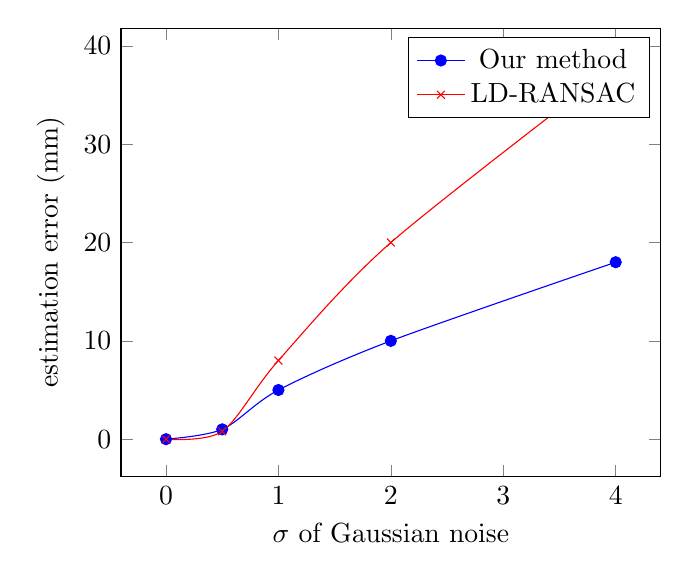
\begin{tikzpicture}
    \begin{axis}[xlabel=$\sigma$ of Gaussian noise, ylabel=estimation error (mm)]
      \addplot[smooth, mark=*, blue] plot coordinates {
        (0, 0)
        (0.5,1)
        (1, 5)
        (2, 10)
        (4, 18)
      };
      \addlegendentry{Our method}
      \addplot[smooth, mark=x, red] plot coordinates {
        (0, 0)
        (0.5,0.8)
        (1, 8)
        (2, 20)
        (4, 38)
      };
      \addlegendentry{LD-RANSAC}
    \end{axis}
  \end{tikzpicture}
  \caption{匹配误差随噪声变化曲线}
  \label{fig:err-noise}
\end{figure}
图中可以看出本文的方法比LD-RANSAC算法有更小的误差,并且对噪声也具有高强的鲁棒性。

为了考察算法的时间性能,通过对输入数据进行降采样(uniform sampling),变化uniform sampling的采集间距来变化输入点云的数量大小,不同点云数量大小下算法的运算时间的变化曲线如图\ref{fig:time-size}所示。
\begin{figure}[ht]
  \centering
  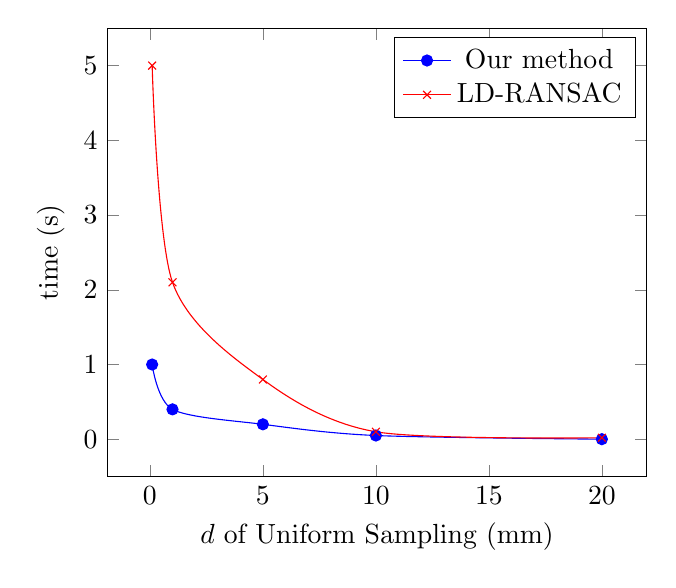
\begin{tikzpicture}
    \begin{axis}[xlabel=$d$ of Uniform Sampling (mm), ylabel=time (s)]
      \addplot[smooth, mark=*, blue] plot coordinates {
        (0.1, 1)
        (1,0.4)
        (5, 0.2)
        (10, 0.05)
        (20, 0.001)
      };
      \addlegendentry{Our method}
      \addplot[smooth, mark=x, red] plot coordinates {
        (0.1, 5)
        (1,2.1)
        (5, 0.8)
        (10, 0.1)
        (20, 0.02)
      };
      \addlegendentry{LD-RANSAC}
    \end{axis}
  \end{tikzpicture}
  \caption{匹配时间随点云数量大小变化曲线}
  \label{fig:time-size}
\end{figure}
图中可以看出本文所设计的方法的运算时间比LD-RANSAC少,并且随着点云数量的增加其运算时间的差距越来越大。

综上,本文所设计的匹配方法相比LD-RANSAC算法具有更高的匹配精度,对噪声的鲁棒性也更强,并且算法的时间复杂度也更小。

\section{3D-MRAI算法流程}
设计完检测模块和匹配模块后,整个3D-MRAI算法就比较简单了,其完整的算法流程如算法\ref{alg:3d-mrai}所示。
\begin{algorithm}
  \caption{3D-MRAI算法}
  \label{alg:3d-mrai}
  \KwIn{RGB Image $I$, Depth Map $D$, CAD Models $M$}
  \KwOut{Set of Pose and Class $Res$}
  $Res\leftarrow \varnothing$\;
  $P\leftarrow \varnothing$\;
  \ForAll {$M_i\in M$} {
    $P\leftarrow \left\{P, CAD2PointCloud(M_i)\right\}$\;
  }
  $H = Depth2HHA(D)$\;
  $Q = Depth2PointCloud(D)$\;
  $Mask, Class \leftarrow DetectModule(I, H)$\;
  \ForAll {$m_i\in Mask, c_i\in Class$} {
    $Q_i \leftarrow Crop(Q, m_i)$\;
    $P_i \leftarrow P(c_i)$\;
    $T_i,S_i\leftarrow MatchModule(P_i, Q_i)$\;
    \If {$S_i > S_{min}$} {
      $Res\leftarrow \left\{Res, \left[T_i, c_i\right]\right\}$\;
    }
  }
  \Return $Res$
\end{algorithm}

3D-MRAI算法首先会将目标的CAD模型转为匹配所需的点云。具体如何转换的话,基本思想是参考Uniform Sampling算法,Uniform Sampling算法的核心思想是以3D栅格中所有点的质心代替这些点,从而达到降采样。类似地,对于CAD模型也建立3D栅格,但由于无法获得3D栅格总所有点,因此判断CAD模型是否穿过3D栅格,如果穿过3D栅格,则在该3D栅格中心出增加一个点。显然3D栅格的边长越大,转换后的点云数量越小,精度越低,考虑到所使用相机生成点云的精度,因使CAD模型转换后的点云的精度与相机采集的点云的精度近似,实际取3D栅格边长为1mm,一个实际工件的CAD模型和以1mm为边长进行采样转换后的模型点云如图\ref{fig:model-pc}所示。
\begin{figure}[ht]
  \centering
  \subfloat[原CAD模型]{\includegraphics[width=7cm]{object-model}}
  \hskip1cm
  \subfloat[转换后点云]{\includegraphics[width=6cm]{object-pointcloud}}
  \caption{CAD模型和转换后的点云}
  \label{fig:model-pc}
\end{figure}

然后3D-MRAI算法会通过深度图计算HHA图和点云,由深度图计算HHA图的算法上文已经详细叙述过了,此处不再复述;将深度图变换为点云这一步则相对简单,只要通过深度摄像头的内参矩阵反投影到三维空间即可,详细见第~\ref{chap:rgbd}~章中RGB-D相机的数学模型。

处理完这些数据后,输入RGB图像和HHA图到检测模块,通过检测模块得到目标物体的BBox/Mask。然后根据BBox/Mask从深度图对应的点云中抠出目标点云,由于深度图转换的点云是有序的,因此BBox/Mask在深度图中的索引坐标与深度图转换的点云的索引坐标是一致的,只要将点云中对应的点提取出来就行,并滤去无效的点然后适当降采样即可,尽管滤波和降采样之后的目标点云是无序的,但后续匹配算法并不需要输入点云有序,而且降采样后点云数量减少,将会减少后续匹配算法的时间。


裁剪得到目标物体的点云$Q_i$后,找出对应物体的CAD模型转换的点云$P_i$,将$P_i$和$Q_i$输入到匹配模块,即可得到CAD模型到目标点云之间的刚体变换$T_i$,由于CAD模型坐标系与相机坐标系重叠,因此将矩阵$T$转换为$X,Y,Z,r,p,y$就是目标点云在相机坐标系下的位姿Pose,最后将所有匹配得到的结果与目标检测的结果组合,并滤去匹配或检测分数较低的结果。

\section{3D目标位姿估计实验}
为了评价所提出的3D-MRAI的性能,设计了3D目标位姿估计的实验,并与文献\cite{hinterstoisser2012model}所提出的基于LINEMOD算法的3D目标位姿估计框架相比较。
\subsection{数据集}
实验所使用的数据集是workpiece数据集,前文已经部分介绍过了,该数据集是在实验室采集的三类物体,检测模块实验中所用workpiece数据集中的ground truth是物体的种类、BBox和Mask,workpiece数据集中测试集中的图片的ground truth除了物体的种类、BBox和Mask,还有物体的位姿,物体的位姿是通过在物体旁固定标定板采集的。具体方法是,通过固定标定板在目标物体旁,我们可以记录标定板到目标的刚体变换关系$T_1$,然后我们通过彩色摄像头可以检测出标定板的位姿$T_2$,则物体的位姿可以通过下式得到
\begin{equation}
  T = T_2T_1
\end{equation}

\subsection{实验内容}
为了有效的评价3D-MRAI算法,我们先定义一个合适的评价指标{\kai 姿态误差}:
\begin{equation}
  m = {\underset{\mathbf{x}\in M}{avg}} \; {\parallel (R\mathbf{x}+t) - (\tilde{R}\mathbf{x}+\tilde{t})\parallel}
\end{equation}
其中$M$表示算法运行结果得到的物体种类对应的CAD模型转换得到的点云,$R$和$t$分别表示从ground truth物体位姿分解得到的旋转变换和平移变换,$\tilde{R}$和$\tilde{t}$分别表示从算法运行结果得到的物体位姿分解得到的旋转变换和平移变换。显然,如果算法运行结果和ground truth越接近,所定义的姿态误差就越小。对于一些对称的物体(如圆柱体的被子),显然不同角度下相机看到的目标物体可能近似,会造成算法运行的结果正确的情况下与ground truth相差很大,造成姿态误差很大,与我们所定义的评价指标的宗旨相违背。因此,针对一些对称的物体,重新定义姿态误差为
\begin{equation}
  m = {\avg_{\mathbf{x}_1\in M}} \; {\min_{\mathbf{x}_2\in M}} \; \norm{(R\mathbf{x}_1+t) - (\tilde{R}\mathbf{x}_2+t)}
\end{equation}
此外,如果$k_md>m$,我们就认为目标物体准确检测到了,并且估计的位姿正确,其中$d$是目标物体对应模型的直径,$k_m$是系数。因此,还可以定义一个正确检测目标并正确估计目标位姿的准确率。

实验在workpiece数据集的测试集上分别运行了3D-MRAI和文献\cite{hinterstoisser2012model}中的基于LINEMOD算法的检测框架,运行实验的计算机有两块Intel(R) Xeon(R) E5-2683 v3(2.00GHz)的CPU,4块TITAN X GPU,由于3D-MRAI有深度神经网络所以使用了一块GPU和一块CPU,Hinterstorisser等人的算法不需要GPU,只使用了一块CPU。

\subsection{实验结果}
\begin{figure}[ht]
  \centering
  \subfloat{\includegraphics[height=3.4cm]{3dmrai-res1}}
  \hskip0.2cm
  \subfloat{\includegraphics[height=3.4cm]{3dmrai-res2}}
  \hskip0.2cm
  \subfloat{\includegraphics[height=3.4cm]{3dmrai-res3}}
  \caption{3D-MRAI运算结果可视化图}
  \label{fig:3dmrai-res}
\end{figure}
3D-MRAI算法在workpiece数据集上一些测试用例的运算结果可视化如图\ref{fig:3dmrai-res}所示。变化系数$k_m$,根据3D-MRAI和Hinterstoisser等人的算法在测试集上的运行结果,统计算法的准确率如表\ref{tab:mrai}所示。
\begin{table}[ht]
  \centering
  \caption{3D-MRAI和Hinterstorisser等人的算法准确率}
  \begin{tabular}{ccccccc}
    \toprule
    $k_m[\%]$&5&7&9&11&13&15\\
    \midrule
    Hinterstorisser et al.&75.63& 83.84& 89.13& 93.48& 96.83&98.12\\
    \bf{3D-MRAI}&95.12& 97.35& 98.10& 98.69& 99.22& 100.00\\
    \bottomrule
  \end{tabular}
  \label{tab:mrai}
\end{table}
\begin{figure}[ht]
  \centering
     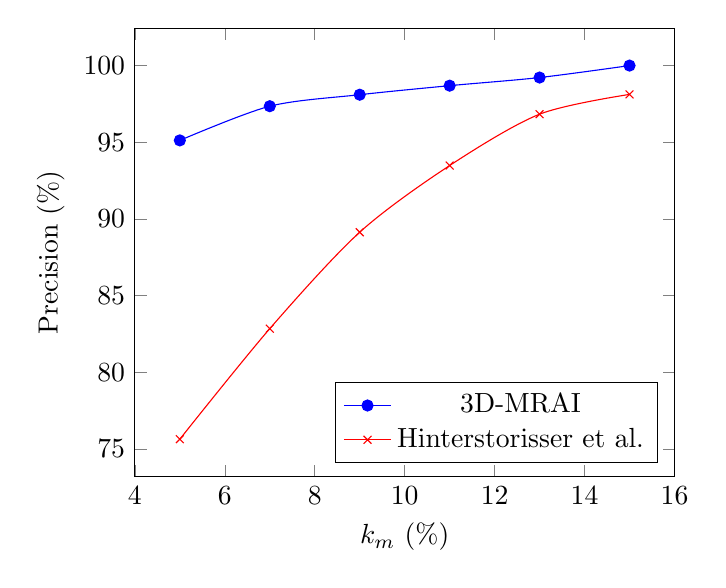
\begin{tikzpicture}
       \begin{axis}[xlabel=$k_m$ (\%),
         ylabel=Precision (\%),
         legend pos=south east,]
         \addplot[smooth, mark=*, blue] plot coordinates {
           (5, 95.12)
           (7, 97.35)
           (9, 98.1)
           (11, 98.69)
           (13, 99.22)
           (15, 100.00)
         };
         \addplot[smooth, mark=x, red] plot coordinates {
           (5, 75.63)
           (7, 82.84)
           (9, 89.13)
           (11, 93.48)
           (13, 96.83)
           (15, 98.12)
         };
         \legend{3D-MRAI,Hinterstorisser et al.}
       \end{axis}
     \end{tikzpicture}
  \caption{3D-MRAI和Hinterstorisser等人的算法准确率曲线}
  \label{fig:mrai}
\end{figure}
表中$k_m$从$5\%$变化到$15\%$,表示物体直径的占比,$k_m$越大,允许的姿态误差就越大,因此准确率就越高。实际实验时,发现$k_m\approx 10\%$时基本上肉眼可以看出匹配的姿态误差。将表\ref{tab:mrai}绘制成图如\ref{fig:mrai}所示,从图中可以发现本文所提出的3D-MRAI算法的准确率大大超过了Hinterstorisser等人的算法,在$k_m=13\%$是3D-MRAI算法的准确率已经接近$100\%$了,以肉眼可以看出匹配的姿态误差$k_m=9\%$为标准时3D-MRAI算法的准确达到了$98.10\%$,比Hinterstorisser等人提出的算法高了大约$9$个百分点。

为了进一步观察算法给出位姿的精度,取$k_m=9\%$时3D-MRAI准确检测的例子,将目标物体的位姿转换为$X,Y,Z,r,p,y$六个直观的变量三维位置和姿态欧拉角,然后于ground truth相比较,得到算法结果在距离和角度上的误差的频率直方图如图\ref{fig:pose-error}所示。
\begin{figure}[ht]
  \centering
  \includegraphics[width=16cm]{pose-error}
  \caption{3D-MRAI算法精度}
  \label{fig:pose-error}
\end{figure}
从图中可以看出3D-MRAI正确检测和估计目标位姿的情况下,在$X,Y,Z$方向下的位置误差大部分分布在$0\sim 1mm$之间,其距离精度在$1mm$左右;在$r,p,y$三个角度下的角度误差也大部分分布在$0\sim 1deg$之间,其角度精度在$1deg$左右。统计图\ref{fig:pose-error}中的数据,可以算出距离误差和角度误差的的均值和方差为:
\begin{equation}
  \begin{array}{ccc}
    e_d &=& 0.82\pm0.21mm\\
    e_a &=& 0.91\pm0.29deg
  \end{array}
\end{equation}

除了关心算法的准确率和精度,算法的运行时间也是我们所关心的。在实验所用的计算机上,本文所设计的3D-MRAI算法与Hinterstorisser等人设计的基于LINEMOD算法的平均帧率如表\ref{tab:mrai-fps}所示。
\begin{table}[ht]
  \centering
  \caption{3D-MRAI和Hinterstorisser等人的算法FPS}
  \begin{tabular}{ccc}
    \toprule
    &Hinterstoisser et al.&\bf{3D-MRAI}\\
    \midrule
    FPS&7.6&2.2\\
    \bottomrule
  \end{tabular}
  \label{tab:mrai-fps}
\end{table}
表中可以看出3D-MRAI的FPS相比Hinterstorisser等人的算法的FPS相对较低,由于使用了深度神经网络相关的算法,涉及到较大的计算量,因此较低的FPS也在情理之中。

综上所述,在$k_m=9\%$时,3D-MRAI算法的准确率为$98.10\%$左右,其估计的位姿的距离精度为$0.82\pm0.21mm$,角度精度为$0.91\pm0.29deg$。

\section{本章小结}
本章介绍了一种基于RGB-D图像的3D目标检测和位姿估计算法3D-MRAI,3D-MARI的核心由检测模块和匹配模块构成。检测模块在Mask R-CNN的基础上通过引入HHA和STN实现在RGB-D图中检测出目标的Mask;匹配模块在4PCS算法的基础上通过点云匹配计算出目标位姿。最后还通过实验与Hinterstorisser等人的算法比较,得出3D-MRAI算法具有更高的检测准确率,并且位姿精度也更高,但在时间性能上略逊于Hinterstorisser等人的算法。

%%% Local Variables:
%%% mode: latex
%%% TeX-master: "../thesis"
%%% End:

% %!TEX root = ../thesis.tex
\chapter{基于RGB-D图像的目标检测算法}
\label{chap:detector}
本章主要介绍所提出的两种基于RGB-D图像的目标检测算法3D Faster R-CNN和3D Mask R-CNN。3D Faster R-CNN是在Faster R-CNN\cite{Ren}的基础上,通过引入深度图以解决单从RGB图难以检测缺少纹理物体(Textureless Object)的问题,并且还引入了Spatial Transformer结构使得提取的特征具有旋转不变性。由于3D Faster R-CNN目标检测的结果是框出目标的Bounding Box,因此使得一些框住细长目标的Bounding Box内大部分像素并不属于该目标,这就使得后面的点云匹配算法难以得到满意的结果。因此3D Mask R-CNN根据Mask R-CNN\cite{He2017}对Faster R-CNN的改进思路,对3D Faster R-CNN进行了改进,使得其不仅能得到目标的Bounding Box,还能得到目标的Mask(可以知道Bounding Box内属于检测目标的像素),大大减少了后续匹配算法的难度。

\section{3D Faster R-CNN}
相比于Faster R-CNN,本文所提出的3D Faster R-CNN主要增加对深度信息的处理和Spatial Transformer,分别用于解决Faster R-CNN在实际应用时所不能解决的问题:
\begin{itemize}
\item 难以检测出缺少纹理的物体
\item 对物体的旋转敏感,提取的特征不具有旋转不变性
\end{itemize}

对于缺少纹理的物体,单从RGB图中很难检测出目标,这是一个很显然的问题,但是现在我们可以从对偶RGB-D相机中获取深度图,对于纹理少的物体,可以从深度图中提取特征检测出目标,所以现在的关键问题是如何从深度图中提取特征,并结合到Faster R-CNN中,本文所提出的方法是将深度图转换到HHA,然后再使用CNN提取特征,具体后文会详细介绍。

Faster R-CNN对于物体旋转敏感的问题,归根到底是因为CNN所提取的特征不具有旋转不变性,实际出现这种问题的情况,如图\ref{fig:cat}所示,
\begin{figure}[!ht]
  \centering
  \subfloat[检测旋转前的图片]{\includegraphics[width=4cm]{cat_up}}
  \hskip1em
  \subfloat[检测旋转后的图片]{\includegraphics[width=4cm]{cat_down}}
  \caption{Faster R-CNN检测识别宠物猫示例}
  \label{fig:cat}
\end{figure}
其中图(b)只是将图(a)旋转了180度,由于CNN所提取的特征不具有旋转不变性,并且训练所实验的图片中的宠物都是头朝上的,即使图(a)在训练集中,将其旋转180度后,也无法从中检测出目标来。解决这个问题有两个思路:
\begin{itemize}
\item Data Augmentation
\item Spatial Transformer
\end{itemize}
Data Augmentation是通过对训练集中的图片进行旋转以获取不同角度的图片,通过这种方式增大数据集从而使得最终训练得到的模型对各种角度的图片都能识别;Spatial Transformer是一种特殊的网络结构,本文所使用的就这种方式,后文会详细介绍。

\subsection{HHA}

\subsection{Faster RCNN}

\subsection{Spatial Transformer}


\section{3D Mask RCNN}

\section{目标检测实验}

\section{本章小结}


% \chapter{基于4PCS的点云匹配算法}
\label{chap:matcher}
本章主要介绍为了估计目标的位姿所提出的一种基于4PCS的点云匹配算法A4PCS-ICP(Angle-fixed-4PCS-ICP),A4PCS-ICP主要基于全局匹配算法4PCS\cite{aiger20084}和局部匹配算法ICP\cite{besl1992method}。为了详细介绍A4PCS-ICP算法,本章首先从整体上简单介绍了A4PCS-ICP算法,包括算法所要解决的问题的具体数学描述以及相关算法的背景;然后介绍A4PCS-ICP算法的基础4PCS算法,并分析了其不足,进而提出A4PCS算法对其进行改进;接着介绍与A4PCS算法相结合的ICP算法,ICP算法主要用于提高最终点云匹配的精度;最后进行了点云匹配的实验,将本文的A4PCS-ICP算法与其他几个匹配算法相比较。

\section{点云匹配算法概述}
\subsection{问题描述}
通过第~\ref{chap:detector}~章中的目标检测算法可以得到目标的bounding box或者mask,根据bounding box或者mask可以在深度图中提取对应的区域,从而获得包含目标的点云。所以现在的问题是如何通过目标的点云计算出目标的位姿,由于可以得到目标的三维模型,因此将目标的三维模型经过一个刚体变换$T$,使之与目标点云重合,然后目标的三维模型在相机坐标系下的位姿也是已知并且可调的,为方便起见将三维模型坐标系与相机坐标系重合,则目标的位姿便等于三维模型与目标点云之间的齐次变换关系,即$T$。所以,要计算目标的位姿,就要求解目标三维模型与相机采集到的目标点云之间的刚体变换$T$,如图~\ref{fig:match_diagram}~,这也是A4PCS-ICP主要要解决的问题:两个点云之间的匹配问题。
\begin{figure}[ht]
  \centering
  \includegraphics[width=14cm]{match_diagram}
  \caption{位姿估计示意图}
  \label{fig:match_diagram}
\end{figure}

相机所采集到的目标点云是一组包含空间三维坐标(x,y,z)以及颜色(r,g,b)的点集\footnote{对点集(point set)与点云(point cloud)不做区分,都指包含坐标点的集合},由于此处并不需要颜色信息,因此对目标点云只保留空间位置信息,去除颜色信息后的目标点云记为点集$P$。三维模型亦可通过采样得到一组包含空间三维坐标的点集,记为$Q$。A4PCS-ICP算法就可以简化为求解一个刚体变换$T$使得点集$P$中的点经过矩阵$T$变换后,尽可能与点集$Q$重合。更为准确地,A4PCS-ICP算法就可以简化为求解一个LCP(Largest Common Pointset)问题:

{\kai LCP问题:给定两个点集$P$和$Q$,在给定距离误差$\delta$下,求解点集$P$的最大子集$P'$,使得$T(P')$和点集$Q$之间的距离在合适的距离度量下小于$\delta$,其中$T$是一个刚体变换。}

\subsection{背景介绍}
LCP问题并不是一个新的问题,解决该问题的算法也有很多,尤其是近些年来,随着几何扫描相关技术的发展,如何将多次扫描或者多个设备采集的三维信息统一到一个坐标系下成为研究的热点,其本质上可以归结为LCP问题或其衍生问题,这些问题是计算机几何学和计算机视觉中的基础问题。

其中一个比较流行的算法是通过使用稳定的局部几何描述子来匹配得到粗略的刚体变换,然后紧接着使用ICP算法迭代获取较为精确的刚体变换\cite{li2005multiscale}。这种算法的效果十分取决于所选取的描述子,通常一般的描述子对传感器噪声都比较敏感,尤其是一些低精度的传感器,常用的局部几何特征描述子有SHOT\cite{salti2014shot}、FFPH\cite{rusu2009fast}等;还有一种比较流行的方法是通过几何希哈方法从事先设置好的候选集中来选择合适的刚体变换\cite{wolfson1997geometric};一些随机算法,如RANSAC(Random Sample Consesue)\cite{bolles1981ransac}通常需要足够长的时间才能保证得到合适的解。

上述介绍的一些算法,有些对噪声的鲁棒性不强,有些时间复杂度极高,有些也难以处理部分重叠的情况,即点集$P$和$Q$之间只有一部分点集是相匹配的,因此难以实际直接应用到本文所需要解决的问题,其效果也难以让人满意。对此,本文基于4PCS(4-Points Congruent Sets)算法设计了有效解决点云匹配的算法A4PCS-ICP。

\section{A4PCS-ICP算法}
\subsection{算法框架}
A4PCS-ICP算法基于4PCS,针对4PCS的瓶颈,有效地降低了其时间复杂度,然后通过与ICP算法配合提高匹配的精度,其整体框架如图~\ref{fig:4pcs-pe}~所示。
\begin{figure}[ht]
  \centering
  \includegraphics[width=12cm]{4pcs-pe}
  \caption{A4PCS-ICP算法框架}
  \label{fig:4pcs-pe}
\end{figure}
A4PCS-ICP由三个模块组成:Angle-fixed 4PCS、Outlier filter和ICP,Angle-fixed 4PCS是4PCS算法的优化版,也是A4PCS-ICP算法的核心,根据输入的两个点集,输出两个点集之间的粗略的变换关系;Outlier filter根据Angle-fixed 4PCS的输出对点集$P'$和$Q'$进行滤波,去掉一些离群点,用以提高下一步ICP算法的精度;ICP模块通过以Angle-fixed filter输出的变换关系为初始值对滤波后的两个点集进行迭代求解最佳的刚体变换关系,输出最终的变换关系$T$,也是目标的位姿。

\subsection{Angle-fixed 4PCS算法}
介绍Angle-fixed 4PCS算法之前,首先先详细介绍一下4PCS算法,4PCS算法是一个对3D点集全局匹配的算法,即使所给的两个3D点集有小的重叠,4PCS都能给出较好的结果,并且对噪声有一定的鲁棒性。这种方法对初始位姿没有任何要求,其核心是从3D点集中提取出所有与给定平面4-points近似全等的共面4-points,该算法时间复杂度为$O(n^2+k)$,其中$n$是3D点集中点的个数,$k$是提取出的4-points个数。4PCS使用十分广泛,并且引申出许多相关的变种\cite{corsini2013fully}。

\begin{algorithm}
  \caption{4PCS算法}
  \label{alg:4pcs}
  \KwIn{Point sets $P$ and $Q$, measure level $\delta$}
  \KwOut{Rigid transform $T$}
  $h\leftarrow 0$\;
  \For {$i = 1$ to $L$} {
    $B\leftarrow$ SELECTCOPLANARBASE($P$)\;
    $U\leftarrow$ FINDCONGRUENT($B,Q,\delta$)\;
    \ForAll {4-points coplannar sets $U_i\in U$} {
      $T_i\leftarrow$ best rigid transform that aligns $B$ to $U_i$ in the least square sense\;
      Find $S_i\subseteq P$, such that $d(T_i(S_i), Q)\leq\delta$\;
    }
    $k\leftarrow arg\;\underset{i}{max}\left\{|S_i|\right\}$\;
    \If {$|S_k| > h$} {
      $h\leftarrow |S_k|$\;
      $T\leftarrow T_k$\;
    }
    \Return $T$\;
  }
  \BlankLine
  \BlankLine
  \BlankLine
  \BlankLine
  \SetKwProg{Def}{def}{:}{}
  \Def{FINDCONGRUENT($B\equiv\left\{\mathbf{b_1},\mathbf{b_2},\mathbf{b_3},\mathbf{b_4}\right\},Q,\delta)$} {
    $d_1\leftarrow\;\parallel\mathbf{b_1}-\mathbf{b_2}\parallel$\;
    $d_2\leftarrow\;\parallel\mathbf{b_3}-\mathbf{b_4}\parallel$\;
    计算$R_1\equiv\left\{(\mathbf{p}_i,\mathbf{p}_j)\;|\;\mathbf{p}_i,\mathbf{p}_j\;\in Q\right\}$,使得$\parallel\mathbf{p}_i-\mathbf{p}_j\parallel\;\in [d_1-\delta,d_1+\delta]$\;
    计算$R_2\equiv\left\{(\mathbf{p}_i,\mathbf{p}_j)\;|\;\mathbf{p}_i,\mathbf{p}_j\;\in Q\right\}$,使得$\parallel\mathbf{p}_i-\mathbf{p}_j\parallel\;\in [d_2-\delta,d_2+\delta]$\;
    \ForAll {$r_{1i}\in R_1$} {
      计算与定量$r_1$和$r_2$相关的四个点$\left\{\mathbf{e}_{1i}^1,\mathbf{e}_{1i}^2,\mathbf{e}_{1i}^3,\mathbf{e}_{1i}^4\right\}$,记$\Pi(\mathbf{e}_{1i}^j)=r_{1i}$\;
    }
    对点集$\left\{\mathbf{e}_{1i}^j\right\}$在$\mathbb{R}^3$空间建立range tree的数据结构\;
    \ForAll {$r_{2i}\in R_1$} {
      计算与定量$r_1$和$r_2$相关的四个点$\left\{\mathbf{e}_{2i}^1,\mathbf{e}_{2i}^2,\mathbf{e}_{2i}^3,\mathbf{e}_{2i}^4\right\}$,记$\Pi(\mathbf{e}_{1i}^j)=r_{1i}$\;
    }
    $U'\leftarrow\varnothing$\;
    \ForAll {$\mathbf{e}_{2i}^j$} {
      在range tree中以$\delta$为领域检索点$\mathbf{e}_{2i}^j$附近的点,对于每个检索到的点$\mathbf{q}$,建立与$B$相对应的4个点的点集$U'\leftarrow\left\{U',(\Pi(\mathbf{q}),\Pi(\mathbf{e}_{2i}^j))\right\}$\;
    }
    \Return $U'$\;
  }
\end{algorithm}

{\kai 4PCS算法流程}:算法流程如\ref{alg:4pcs}所示,该算法输入两个点集$P$和$Q$,还有距离参数$\delta$,返回两个点集之间的刚体变换$T$。4PCS基于以下事实:{\kai 共面点集中定义的比例在仿射变换,包括刚体运动中保持不变。}举例来说,定义点集$X:=\left\{\mathbf{a},\mathbf{b},\mathbf{c},\mathbf{d}\right\}$,其中4个点不都在同一条直线上,设直线$ab$和$cd$相交于点$\mathbf{e}$,定义两个比例:
\begin{equation}
  \begin{array}{ccc}
    r_1& =& {\parallel \mathbf{a}-\mathbf{e}\parallel}/{\parallel \mathbf{a}-\mathbf{b}\parallel}\\
    r_2& =& {\parallel \mathbf{c}-\mathbf{e}\parallel}/{\parallel \mathbf{c}-\mathbf{d}\parallel}
  \end{array}
\end{equation}
则在仿射变换下所定义的$r_1$和$r_2$均保持不变,如图\ref{fig:4points}。
\begin{figure}[ht]
  \centering
  \includegraphics[width=12cm]{4points}
  \caption{4-points比例的仿射不变性}
  \label{fig:4points}
\end{figure}
如果曲面$S_1$和$S_2$匹配,并且4-points共面基在重叠区域,则$\mathbf{a},\mathbf{b},\mathbf{c},\mathbf{d}$对应的四个点$\mathbf{a}',\mathbf{b}',\mathbf{c}',\mathbf{d}'$也共面,并且
\begin{equation}
  \begin{array}{ccc}
    {\parallel \mathbf{a}'-\mathbf{e}'\parallel}/{\parallel \mathbf{a}'-\mathbf{b}'\parallel}&=&r_1\\
    {\parallel \mathbf{c}'-\mathbf{e}'\parallel}/{\parallel \mathbf{c}'-\mathbf{d}'\parallel}&=&r_2\\
  \end{array}
\end{equation}


4PCS算法另一个关键技术是使用了{\kai 宽基}(\emph{wide-base}),相比于一般的基,宽基中基的长度更长,如图\ref{fig:wide-base}所示,图片上半部分是使用宽基匹配的曲线,图片下半部分是使用一般的基匹配的曲线,显然,通过比较可以发现宽基相比普通基有更稳定的匹配结果,相关理论证明见文献\cite{goodrich1994practical}。
\begin{figure}[ht]
  \centering
  \includegraphics[width=14cm]{wide-base}
  \caption{宽基的匹配稳定性}
  \label{fig:wide-base}
\end{figure}

回到4PCS算法具体实现,算法的主体其实是一个RANSAC循环,每次循环首先会从点集$P$中挑选共面的宽基$B$,具体实现时,先从点集$P$中随机选取3个点,然后在剩下的点中选取第四个点构成共面的四点,第四个点的选取尽可能使得每个点之间的距离最大(因为我们要使用宽基),并且与前3个点近似共面(显然由于噪声的存在,完全共面并不现实),但如果第四个点选取的过远也会出现问题,因为如果宽基超过两个点集的重叠区域则难以匹配,因此当选以最大距离取宽基造成误差变大时以$f=1,0.5,0.25,\ldots$的比率降低最大距离来选取宽基。

在点集$P$中选取好宽基$B$后,算法下一步会在点集$Q$中通过4-points的仿射不变性找出所有与宽基$B$“全等”的基,构成集合$U$。在$Q$中选取基的方法见算法\ref{alg:4pcs}中的FINDCONGRUENT函数,函数首先使用基$B$中的点先定义两个仿射无关的比例,如图\ref{fig:findbase}中左边的图所示。
\begin{figure}[ht]
  \centering
  \includegraphics[width=15cm]{findbase}
  \caption{寻找近似“全等”的基示意图}
  \label{fig:findbase}
\end{figure}
假设在点集$Q$中找到两点$\mathbf{q}_1$和$\mathbf{q}_2$,并且$\left|\parallel \mathbf{q}_1-\mathbf{q}_2\parallel - \parallel \mathbf{a}-\mathbf{b}\parallel\right| \leq \delta$,则点$\mathbf{q}_1,\mathbf{q}_2$有可能与点$\mathbf{a}, \mathbf{b}$对应,则直线$\mathbf{a}\mathbf{b}$与$\mathbf{c}\mathbf{d}$相交的点$\mathbf{e}$的对应点可能为
\begin{equation}
  \mathbf{e}_1 = \mathbf{q}_1 + r1(\mathbf{q}_2-\mathbf{q}_1)
\end{equation}
或者
\begin{equation}
  \mathbf{e}_1 = \mathbf{q}_2 + r1(\mathbf{q}_1-\mathbf{q}_2)
\end{equation}
同理也可以根据$\mathbf{c},\mathbf{d}$的对应点(设为$\mathbf{q}_3, \mathbf{q}_4$)求得$\mathbf{e}$的对应点
\begin{equation}
  \mathbf{e}_2 = \mathbf{q}_3 + r1(\mathbf{q}_4-\mathbf{q}_3)
\end{equation}
或者
\begin{equation}
  \mathbf{e}_2 = \mathbf{q}_4 + r1(\mathbf{q}_3-\mathbf{q}_4)
\end{equation}
则当$\mathbf{e}_1\approx \mathbf{e}_2$时,$\mathbf{q}_1,\mathbf{q}_2,\mathbf{q}_3,\mathbf{q}_4$就是我们所要找的一组与点$\mathbf{a},\mathbf{b},\mathbf{c},\mathbf{d}$近似“全等”的基,如图\ref{fig:findbase}中右边图中的$\mathbf{q}_5,\mathbf{q}_3,\mathbf{q}_4,\mathbf{q}_1$。

具体实现时,当我们在点集$Q$中找出了所有可能的$\mathbf{e}_1$和$\mathbf{e}_2$后,找出其中近似相等的$\mathbf{e}_1$和$\mathbf{e}_2$可以通过range树\cite{arya1998optimal}来实现,对于大小为$n$的点集,range树的建立时间复杂度为$O(n\lg n)$,查询附近点的时间复杂度为$O(\lg n + k)$,其中$k$是查询到点的个数。

在$Q$中找出所有与基$B$近似“全等”的基后,下一步就是计算出最优的刚体变换$T$。对于$U$中的每个基$U_i$,我们可以利用最小二乘\cite{horn1987closed}的思想计算$B$到$U_i$的刚体变换$T_i$。得到刚体变换$T_i$后,我们将点集$P$进行变换$T_i$,然后对变换后的点集中的点在$Q$中查找最近点,统计最近点距离小于$\delta$的个数$S_i$,$S_i$也是评价$T_i$效果的分数,分数越高的$T_i$就是我们要求的最优刚体变换$T$。

{\kai 4PCS算法时间复杂度:}设输入的两个点集$P,Q$的大小分别为$m,n$。算法中最耗时的部分是FINDCONGRUENT函数:从点集$Q$中选取距离为$d_1$和$d_2$的点对,其时间复杂度为$O(n^21)$,然后建立和查询range树,其复杂度为$O(n^2+k$,其中$k$是满足条件的基个数,因此4PCS算法整体的时间复杂度为$O(n^2+k)$,空间复杂度显然为$O(n)$。

{\kai 4PCS算法不足:}仔细研究4PCS算法,可以发现从点集$Q$中提取的基与$B$并不是全等的,如图\ref{fig:4pcs-flaw}所示,
\begin{figure}[ht]
  \centering
  \includegraphics[width=12cm]{4pcs-flaw}
  \caption{4PCS中"全等“的基}
  \label{fig:4pcs-flaw}
\end{figure}
将线段$\mathbf{q}_1\mathbf{q}_2$绕交点转动一定角度后便不再与原基全等,但是4PCS仍然会找出点$\mathbf{q}_1',\mathbf{q}_2',\mathbf{q}_3,\mathbf{q}_4$作为与$\mathbf{p}_1',\mathbf{p}_2',\mathbf{p}_3,\mathbf{p}_4$全等的基。这一缺点会导致4PCS算法需要更多的求解时间,并且还有可能影响最终的匹配结果。

@todo: 4pcs算法改进

\subsection{Outlier filter}
从图~\ref{fig:match_diagram}其实可以看出目标点云有许多点并不属于目标物体,尤其是检测结果没有mask只能使用bbox分割目标时,不属于目标物体的离群点就尤其的多。因此,为了提高最终的匹配精度,除去这些离群点十分有必要,Outlier filter模块的作用就是根据Angle-fixed 4PCS输出的初始刚体变换来去除点云数据中的离群点,从而提升下一步ICP算法匹配的精度,使最终估计的位姿精度提高。

Outlier filter模块的核心算法如算法\ref{alg:outlier-filter}所示。
\begin{algorithm}[ht]
  \caption{Outlier filter算法}
  \label{alg:outlier-filter}
  \KwIn{Point sets $P$ and $Q$, Initial transform $T$, Distance tolerance $\delta$}
  \KwOut{Point sets $P'$ and $Q'$}
  $P'\leftarrow P$\;
  $Q'\leftarrow \varnothing$\;
  \ForAll {point $\mathbf{p}_i\in P$} {
    $\mathbf{p}_i\leftarrow T(\mathbf{p}_i)$\;
  }
  对点集$P$在$\mathbb{R}^3$空间建立kd树的数据结构\;
  \ForAll {point $\mathbf{q}_i\in Q$} {
    在kd树中检索出距离点$\mathbf{q}_i$最近的点$\mathbf{p}$\;
    $d\leftarrow\;\parallel\mathbf{q}_i-\mathbf{p}\parallel$\;
    \If {$d \leq \delta$} {
      $Q'\leftarrow \left\{Q', \mathbf{q}_i\right\}$\;
    }
  }
  \Return $P'$,$Q'$\;
\end{algorithm}
算法输入点集$P$和$Q$,需要参数初始刚体变换$T$,以及允许的距离误差$\delta$,由于点集$P$是由物体的CAD模型转换过来的,因此不对其进行滤波,只对点集$Q$进行离群点去除。具体方法是,首先使用$T$对点集$P$进行刚体变换;然后对变换后的点集建立kd树,建立kd树的目的是为了快速在点集$P$中找到距离某点最近的点,其查找的时间复杂度为$O(kN^{1-1/k}$,其中$k$是所建立kd树的维数,显然对于三维空间中点集为3,$N$是建立的kd树的节点个数;建立好kd树后,对点集$Q$中的每个点在kd树中找到与之距离最近的点,如果两点间的距离大于所设的参数$\delta$,则在点集Q中去除该点。实际运行Outlier filter算法的效果如图\ref{fig:outlier-filter}所示。
\begin{figure}[ht]
  \centering
  \includegraphics[width=13cm]{outlier-filter}
  \caption{Outlier filter效果图}
  \label{fig:outlier-filter}
\end{figure}


\subsection{ICP算法}
ICP(Iterative Closest Point)算法,即最近点迭代算法,是最为经典的数据配准算法。ICP算法本质上是基于最小二乘法的最优配准方法。该算法重复进行选择对应关系点对,计算最优刚体变换,直到满足正确配准的收敛精度要求。由于ICP算法是一种迭代算法,因此只要时间允许便可以获取足够精度的解,但也正因为如此,ICP也容易陷入局部最优解。本文充分考虑了ICP算法的这个特点,通过Angle-fixed 4PCS算法给出初始的刚体变换来避免ICP算法陷入局部最优解,同时通过迭代来提高最后输出的刚体变换精度。下面介绍一下ICP算法的基本原理。

给定两个点集$P_n:=\left\{\mathbf{p}_1,\mathbf{p}_2,\ldots,\mathbf{p}_n\right\}$和$Q_m:=\left\{\mathbf{q}_1,\mathbf{q}_2,\ldots,\mathbf{q}_m\right\}$,以及初始旋转变换$R$和平移变换$t$,以及迭代结束额距离误差$\delta$,ICP算法迭代步骤如下:
\begin{itemize}
\item {\kai 步骤1:}根据当前$R$和$t$,对于点集$P_n$中的每个点在$Q_m$中找出距离最近的点,构成点集$Q_n$;
\item {\kai 步骤2:}计算$P_n$和$Q_n$之间的距离的均方根误差:
  \begin{equation}
    E(R,t) = \frac{1}{n}\sum_{i=1}^n{\parallel \mathbf{q}_i - R\mathbf{p}_i - t\parallel}
  \end{equation}
  通过奇异值分解求得使得$E(R,t)$最小的$R'$和$t'$;
\item {\kai 步骤3:}如果$E(R,t) < \delta$,结束迭代;否则$R\leftarrow R'$,$t\leftarrow t'$,跳转至步骤1。
\end{itemize}

ICP算法的迭代过程还是相对来说十分简单的,唯一需要思考一下的是如何求得最小化$E(R,t)$的$R'$和$t'$,通过奇异值分解求解$R'$和$t'$的方法如下:

首先,记
\begin{equation}
  \left\{
  \begin{array}{ccccc}
  P_n'& = &\left\{\mathbf{p}_i-\mathbf{\mu}_p \;|\; \forall \mathbf{p}_i \in P_n\right\}&:=&\left\{\mathbf{p}'_i\right\}\\
  Q_n'& = &\left\{\mathbf{q}_i-\mathbf{\mu}_q \;|\; \forall \mathbf{q}_i \in Q_n\right\}&:=&\left\{\mathbf{q}'_i\right\}
  \end{array}
  \right.
\end{equation}
其中
\begin{equation}
  \left\{
    \begin{array}{ccc}
      \mathbf{\mu}_p&=&\frac{1}{n}\sum_{i=1}^n{\mathbf{p}_i}\\
      \mathbf{\mu}_q&=&\frac{1}{n}\sum_{i=1}^n{\mathbf{q}_i}
    \end{array}
  \right.
\end{equation}
再另
\begin{equation}
  W = \sum_{i=1}^n{\mathbf{p}_i'\mathbf{q}_i'}
\end{equation}
然后对矩阵$W$进行奇异值分解:
\begin{equation}
  W = U\Sigma V^T
\end{equation}
则
\begin{equation}
  \left\{
    \begin{array}{ccc}
      R'&=&UV^T \\
        t'&=&\mathbf{\mu}_p-R'\mathbf{\mu}_q
    \end{array}
    \right.
\end{equation}

\section{点云匹配实验}
为了评价所设计的算法A4PCS-ICP,考察其匹配精度以及时间性能,本文设计了位姿估计的实验,不但考察了A4PCS-ICP的性能,还与其他一些算法作比较,验证了A4PCS-ICP算法的匹配的精确度。

@todo: 点云匹配实验

\section{本章小结}
@todo: matcher 小结

%%% Local Variables:
%%% TeX-master: "../thesis.tex"
%%% End:
% \chapter{3D目标位姿估计算法}
\label{chap:pose}
本章提出了一种3D目标位姿估计算法3D-MRAI(3D Mask R-CNN \& A4PCS-ICP),该算法根据所提供目标的CAD模型,可以在RGB-D图中检测出目标,并给出目标的位姿。3D-ODPE算法主要基于第~\ref{chap:detector}~章中基于RGB-D图的目标检测算法3D Faster R-CNN/3D Mask R-CNN,以及第~\ref{chap:matcher}~章中的点云匹配算法A4PCS-ICP,通过将这两个算法结合,分两步计算出RGB-D图中目标的位姿。为了评价3D-MRAI算法的性能,本章还设计了相关实验,并与同类算法做了比较。

\section{3D-MRAI框架设计}
3D-MRAI主要解决三维空间中的目标检测和位姿估计问题,根据RGB-D图像,给出图像中目标的种类和其在三维空间中的位姿,区别与常见的在2D图像中的目标检测(如第~\ref{chap:detector}~章中的算法)给出的是目标的种类和其在图像坐标中的bounding box或者mask。给出目标在三维空间中的位姿的意义十分巨大,尤其在机器人领域中,图像层面的结果往往难以满足要求,但难度也很大。

一些给出3D目标位姿的传统算法,如3DMatch\cite{zeng20163dmatch},3DMatch通过匹配局部几何特征来计算目标的位姿,缺点是对采集的3d数据质量要求很高,往往需要使用激光采集,因此整个识别过程的时间很久;通过SIFT描述子来匹配目标位姿\cite{dias2015sift}也是一种方法,但其对纹理较少的物体往往难以匹配,效果很差;另外如LINEMOD\cite{hinterstoisser2012gradient}和MOPED\cite{collet2011moped}这些位姿估计框架,在某些情况下如目标在平整的桌面上并且光照条件较好的情况下才能取得满意的效果。因此,急需一种鲁棒性较强,精度较高,计算时间较短的3D目标位姿估计算法。

3D-MRAI的框架如图\ref{fig:detect-pose}所示,
\begin{figure}[ht]
  \centering
  \includegraphics[width=12cm]{detect-pose}
  \caption{3D-MRAI算法框架}
  \label{fig:detect-pose}
\end{figure}
从图\ref{fig:detect-pose}可以看出算法的输入是RGB图像、深度图,以及目标物体的CAD模型,输出是图像中检测到的目标的位姿。3D-MRAI的核心部分是3D Faster/Mask R-CNN和A4PCS-ICP算法,3D Faster/Mask R-CNN以及在第~\ref{chap:detector}~章详细介绍过,A4PCS-ICP也在第~\ref{chap:matcher}~章详细介绍过了。因此,3D-MRAI估计目标的位姿流程上也是分为两步(two-stage):
\begin{itemize}
\item {\kai 目标检测}:利用3D Faster/Mask R-CNN检测目标,得到目标BBox或者Mask
\item {\kai 点云匹配}:将CAD模型与目标检测对应的点云进行匹配,得到目标位姿
\end{itemize}

\section{3D-MRAI具体实现}
对与3D-MRAI输入的RGB图像和深度图,可以由对偶RGB-D获得,具体见第~\ref{chap:rgbd}~章。目标物体的CAD模型也容易获得,对于工厂中的工件,往往是有其CAD模型的,对于一般物体,可以通过3D扫描仪重构出来,当然也可以使用本文设计的对偶RGB-D相机采集重构出来。

获得目标物体的CAD模型后,为了方便后续需处理,我们需要将其转换为点云。具体如何转换的话,基本思想是参考Uniform Sampling算法,Uniform Sampling算法的核心思想是以3D栅格中所有点的质心代替这些点,从而达到降采样。类似地,对于CAD模型也建立3D栅格,但由于无法获得3D栅格总所有点,因此判断CAD模型是否穿过3D栅格,如果穿过3D栅格,则在该3D栅格中心出增加一个点。显然3D栅格的边长越大,转换后的点云数量越小,精度越低,考虑到所使用相机生成点云的精度,因使CAD模型转换后的点云的精度与相机采集的点云的精度近似,实际取3D栅格边长为1mm,一个实际工件的CAD模型和以1mm为边长进行采样转换后的模型点云如图~\ref{fig:model-pc}~所示。
\begin{figure}[ht]
  \centering
  \subfloat[原CAD模型]{\includegraphics[width=7cm]{object-model}}
  \hskip1cm
  \subfloat[转换后点云]{\includegraphics[width=6cm]{object-pointcloud}}
  \label{fig:model-pc}
  \caption{CAD模型和转换后的点云}
\end{figure}
此外,还需要将深度图转换为点云,这一步则相对简单,只要通过深度摄像头的内参矩阵反投影到三维空间即可,详细见第~\ref{chap:rgbd}~章。

对于3D Faster/Mask R-CNN的输入,还需要将深度图转换为HHA,具体见~\ref{sec:hha}~小节。3D Faster/Mask R-CNN模块的实现,由于一个深度神经网络,只要训练好后将网络模型导出成Tensorflow的pb文件,然后此处导入该网络模型,给定输入,网络输出便是图片中目标的BBox/Mask和Class。

得到目标物体的BBox/Mask后,需要从深度图对应的点云中抠出目标点云,由于深度图转换的点云是有序的,因此BBox/Mask在深度图中的索引坐标与深度图转换的点云的索引坐标是一致的,只要将点云中对应的点提取出来就行,并滤去无效的点然后适当降采样即可,尽管滤波和降采样之后的目标点云是无序的,但后续匹配算法并不需要输入点云有序,而且降采样后点云数量减少,将会减少后续匹配算法的时间。

裁剪得到目标物体的点云$Q_i$后,找出对应物体的CAD模型转换的点云$P_i$,将$P_i$和$Q_i$输入到A4PCS-ICP模型,即可得到CAD模型到目标点云之间的刚体变换$T_i$,由于CAD模型坐标系与相机坐标系重叠,因此将矩阵$T$转换为$X,Y,Z,r,p,y$就是目标点云在相机坐标系下的位姿Pose,最后将所有匹配得到的结果与目标检测的结果组合,并滤去匹配或检测分数较低的结果。详细的算法流程如算法\ref{alg:3d-mrai}所示。
\begin{algorithm}
  \caption{3D-MRAI算法}
  \label{alg:3d-mrai}
  \KwIn{RGB Image $I$, Depth Map $D$, CAD Models $M$}
  \KwOut{Set of Pose and Class $Res$}
  $Res\leftarrow \varnothing$\;
  $P\leftarrow \varnothing$\;
  \ForAll {$M_i\in M$} {
    $P\leftarrow \left\{P, CAD2PointCloud(M_i)\right\}$\;
  }
  $H = Depth2HHA(D)$\;
  $Q = Depth2PointCloud(D)$\;
  $Mask, Class \leftarrow 3DMASKRCNN(I, H)$\tcp*{Same with $3DFASTERRCNN$}
  \ForAll {$m_i\in Mask, c_i\in Class$} {
    $Q_i \leftarrow Crop(Q, m_i)$\;
    $P_i \leftarrow P(c_i)$\;
    $T_i,S_i\leftarrow A4PCSICP(P_i, Q_i)$\;
    \If {$S_i > S_{min}$} {
      $Res\leftarrow \left\{Res, \left[T_i, c_i\right]\right\}$\;
    }
  }
  \Return $Res$
\end{algorithm}

\section{3D目标位姿估计实验}
为了评价所提出的3D-MRAI的性能,设计了3D目标位姿估计的实验,并与文献\cite{hinterstoisser2012model}所提出的基于LINEMOD算法的3D目标位姿估计框架相比。
\subsection{数据集}
实验所使用的数据集是workpiece数据集,在第\ref{sec:dataset}小节中已经部分介绍过了,该数据集是在实验室采集的三类物体,第~\ref{chap:detector}~章中实验所用workpiece数据集中的ground truth是物体的种类、BBox和Mask,workpiece数据集中测试集中的图片的ground truth除了物体的种类、BBox和Mask,还有物体的位姿,物体的位姿是通过在物体旁固定标定板采集的。具体方法是,通过固定标定板在目标物体旁,我们可以记录标定板到目标的刚体变换关系$T_1$,然后我们通过彩色摄像头可以检测出标定板的位姿$T_2$,则物体的位姿可以通过下式得到
\begin{equation}
  T = T_2T_1
\end{equation}

\subsection{实验内容}
为了有效的评价3D-MRAI算法,我们先定义一个合适的评价指标{\kai 姿态误差}:
\begin{equation}
  m = {\underset{\mathbf{x}\in M}{avg}} \; {\parallel (R\mathbf{x}+t) - (\tilde{R}\mathbf{x}+\tilde{t})\parallel}
\end{equation}
其中$M$表示算法运行结果得到的物体种类对应的CAD模型转换得到的点云,$R$和$t$分别表示从ground truth物体位姿分解得到的旋转变换和平移变换,$\tilde{R}$和$\tilde{t}$分别表示从算法运行结果得到的物体位姿分解得到的旋转变换和平移变换。显然,如果算法运行结果和ground truth越接近,所定义的姿态误差就越小。对于一些对称的物体(如圆柱体的被子),显然不同角度下相机看到的目标物体可能近似,会造成算法运行的结果正确的情况下与ground truth相差很大,造成姿态误差很大,与我们所定义的评价指标的宗旨相违背。因此,针对一些对称的物体,重新定义姿态误差为
\begin{equation}
  m = {\avg_{\mathbf{x}_1\in M}} \; {\min_{\mathbf{x}_2\in M}} \; \norm{(R\mathbf{x}_1+t) - (\tilde{R}\mathbf{x}_2+t)}
\end{equation}
此外,如果$k_md>m$,我们就认为目标物体准确检测到了,并且估计的位姿正确,其中$d$是目标物体对应模型的直径,$k_m$是系数。因此,还可以定义一个正确检测目标并正确估计目标位姿的准确率。

实验在workpiece数据集的测试集上分别运行了3D-MRAI和文献\cite{hinterstoisser2012model}中的基于LINEMOD算法的检测框架,运行实验的计算机有两块Intel(R) Xeon(R) E5-2683 v3(2.00GHz)的CPU,4块TITAN X GPU,由于3D-MRAI有深度神经网络所以使用了一块GPU和一块CPU,Hinterstorisser等人的算法不需要GPU,只使用了一块CPU。

\subsection{实验结果}
% @TODO: exp detect results figures
分别统计3D-MRAI和LINEMOD在测试集上的运行结果,变化系数$k_m$统计算法的准确率如表\ref{tab:mrai}所示。
\begin{table}[ht]
  \centering
  \begin{tabular}{ccccccc}
    \toprule
    $k_m[\%]$&5&7&9&11&13&15\\
    \midrule
    Hinterstorisser et al.&75.63& 83.84& 89.13& 93.48& 96.83&98.12\\
    \bf{3D-MRAI}&95.12& 97.35& 98.10& 98.69& 99.22& 100.00\\
    \bottomrule
  \end{tabular}
  \caption{3D-MRAI和Hinterstorisser等人的算法准确率}
  \label{tab:mrai}
\end{table}
表中$k_m$从$5\%$变化到$15\%$,表示物体直径的占比,$k_m$越大,允许的姿态误差就越大,因此准确率就越高。实际实验时,发现$k_m\approx 10\%$时基本上肉眼可以看出匹配的姿态误差。将表\ref{tab:mrai}绘制成图如\ref{fig:mrai}所示,从图中可以发现本文所提出的3D-MRAI算法的准确率大大超过了Hinterstorisser等人的算法,在$k_m=13\%$是3D-MRAI算法的准确率已经接近$100\%$了,以肉眼可以看出匹配的姿态误差$k_m=9\%$为标准时3D-MRAI算法的准确达到了$98.10\%$,比Hinterstorisser等人提出的算法高了大约$9$个百分点。
\begin{figure}[ht]
  \centering
  \includegraphics[width=15cm]{accuracy}
  \caption{3D-MRAI和Hinterstorisser等人的算法准确率曲线}
  \label{fig:mrai}
\end{figure}

为了进一步观察算法给出位姿的精度,取$k_m=9\%$时3D-MRAI准确检测的例子,将目标物体的位姿转换为$X,Y,Z,r,p,y$六个直观的变量三维位置和姿态欧拉角,然后于ground truth相比较,得到算法结果在距离和角度上的误差的频率直方图如图\ref{fig:pose-error}所示。
\begin{figure}[ht]
  \centering
  \includegraphics[width=16cm]{pose-error}
  \caption{3D-MRAI算法精度}
  \label{fig:pose-error}
\end{figure}
从图中可以看出3D-MRAI正确检测和估计目标位姿的情况下,在$X,Y,Z$方向下的位置误差大部分分布在$0\sim 1mm$之间,其距离精度在$1mm$左右;在$r,p,y$三个角度下的角度误差也大部分分布在$0\sim 1deg$之间,其角度精度在$1deg$左右。统计图\ref{fig:pose-error}中的数据,可以算出距离误差和角度误差的的均值和方差为:
\begin{equation}
  \begin{array}{ccc}
    e_d &=& 0.82\pm0.21mm\\
    e_a &=& 0.91\pm0.29deg
  \end{array}
\end{equation}

除了关心算法的准确率和精度,算法的运行时间也是我们所关心的。在实验所用的计算机上,本文所设计的3D-MRAI算法与Hinterstorisser等人设计的基于LINEMOD算法的平均帧率如表\ref{tab:mrai-fps}所示。
\begin{table}[ht]
  \centering
  \begin{tabular}{ccc}
    \toprule
    &Hinterstoisser et al.&\bf{3D-MRAI}\\
    \midrule
    FPS&7.6&2.2\\
    \bottomrule
  \end{tabular}
  \caption{3D-MRAI和Hinterstorisser等人的算法准确率}
  \label{tab:mrai-fps}
\end{table}
表中可以看出3D-MRAI的FPS相比Hinterstorisser等人的算法的FPS相对较低,由于使用了深度神经网络相关的算法,涉及到较大的计算量,因此较低的FPS也在情理之中。

综上所述,在$k_m=9\%$时,3D-MRAI算法的准确率为$98.10\%$左右,其估计的位姿的距离精度为$0.82\pm0.21mm$,角度精度为$0.91\pm0.29deg$。

\section{本章小结}
本章介绍了一种基于RGB-D图像的3D目标检测和位姿估计算法3D-MRAI,3D-MARI通过结合3D Faster/Mask R-CNN和A4PCS-ICP算法实现对目标位姿的估计。并通过实验与Hinterstorisser等人的算法比较,得出3D-MRAI算法具有更高的检测准确率,并且位姿精度也更高,但在时间性能上略逊于Hinterstorisser等人的算法。

%%% Local Variables:
%%% mode: latex
%%% TeX-master: "../thesis"
%%% End:

\chapter{算法应用——Bin-Picking}
\label{chap:app}
本章主要介绍3D-MRAI算法的实际应用——Bin-Picking。首先介绍一下Bin-Picking相关背景,以及近些年的具体研究与发展;然后详细介绍基于3D-MRAI算法所开发的一套解决Bin-Picking问题的视觉系统,包括硬件的选型、开发环境、系统的框架设计以及算法的具体实现;最后介绍了针对所开发的Bin-Picking视觉系统,进行了随机抓取的实验,测试了系统抓取的成功率以及系统的抓取速度。

\section{Bin-Picking背景与现状}
使用机器人分拣散乱的工件的问题,在学术上我们称之为Bin-Picking,Bin-Picking并不是一个崭新的问题,学术上对这个问题的研究以及有了五十多年的历史。典型的Bin-Picking系统主要包括三部分:机器人、视觉检测模块和计算机控制模块。其中,视觉检测模块是整个Bin-Picking系统的核心部分,通过视觉检测模块对存放散乱工件的物料箱进行分析,获取目标工件的位姿,计算机控制模块根据视觉检测模块的检测结果规划机器人的运动路径,然后机器人执行完成工件的抓取。

传统的Bin-Picking中检测估计目标工件的算法大致可以分为两类:一类是基于特征匹配的算法,另一类是基于模板匹配的算法。基于特征匹配的算法,通过某些特征描述目标工件,如边角、空洞等特征,然后通过分析特征在空间中的旋转变换和平移变换来估计目标零件的位姿。这一类方法受工件纹理或者结构以及传感器的精度影响很大。另外一类基于模板匹配的方法的精度受限与模板的数量,要获得较高的精度就需要大量的模板,而大量的模板会造成算法运行时间过长。

工业上用于解决Bin-Picking问题的视觉系统也有许多,如图\ref{fig:bin-picking-sys}所示。日本的Fanuc公司推出了基于iRVision的Bin-Picking系统,该系统通过四个相机进行三维视觉重建,然后进行目标定位\cite{connolly2007new}。德国的ISRA Vision公司推出了3D Shape Scan系统,丹麦的Scape Technologies公司推出了Scape-Tech Discs系统,德国的Sick公司退出了PLB-500系统,诸如类似的Bin-Picking系统还有许多,这些Bin-Picking系统的价格大多二十万以上,并且抓取成功率和速度也往往难以满足客户需求,因此工业上还是缺少成熟的、价格便宜的、抓取成功率高、速度快的Bin-Picking解决方案。
\begin{figure}[ht]
  \centering
  \subfloat[Fanuc的iRVision系统]{\includegraphics[width=6cm]{fanuc}}
  \hskip1.5cm
  \subfloat[ISRA Vision的3D Shape Scan系统]{\includegraphics[width=6cm]{3dshape}}
  \vfill
  \subfloat[Scape Technologies的Scape-Tech Discs系统]{\includegraphics[width=6cm]{scapetech}}
  \hskip1.5cm
  \subfloat[Sick的PLB-500系统]{\includegraphics[width=6cm]{plb500}}
  \caption{工业上典型的Bin-Picking解决方案}
  \label{fig:bin-picking-sys}
\end{figure}

随着近几年一些高性价比的3D相机的出现,如微软的Kinect系列、Intel的RealSense系列,加上近几年深度学习的巨大发展,使得开发一种性价比高的、抓取成功率高的、速度快的Bin-Picking系统成为可能。但尽管深度学习在计算机视觉领域(Computer Vision)有了大量的研究,但在机器人感知(Robot Perception)领域的应用还比较少,因此本文将深度学习在计算机视觉领域内的成果通过一些改进引入到Robot Perception领域,再结合传统的全局点云匹配算法,提除了3D-MRAI算法,可以用于解决Bin-Picking相关问题。此外,本文基于Intel的RealSense SR300相机所提出的对偶RGB-D相机构建也为整个Bin-Picking系统提供了高性价比的相机解决方案。

\section{基于3D-MRAI的随机分拣系统}
\subsection{系统硬件设计}
本文所设计的基于3D-MRAI的随机分拣系统的硬件系统如图\ref{fig:hardware-sys}所示。
\begin{figure}[ht]
  \centering
  \includegraphics[width=14cm]{hardware-sys}
  \caption{基于3D-MRAI的随机分拣系统硬件框架}
  \label{fig:hardware-sys}
\end{figure}
从图\ref{fig:hardware-sys}可以看出,所设计的随机分拣系统的硬件系统由三个部分构成:相机模块、嵌入式计算模块以及机器人模块。对于相机模块,根据3D-MRAI算法的输入,需要相机能采集RGB-D图像,并且考虑整个系统的响应时间以及价格因此,希望相机模块的采集时间尽可能短,性价比尽可能高,因此选用了以结构光为原理的3D相机,并根据第~\ref{chap:rgbd}~章所设计的对偶RGB-D相机,用两个SR300相机构成了对偶RGB-D相机模块。

嵌入式计算模块选用了搭载了NVDIA公司的Jetson TX2模块的嵌入式计算机,如图\ref{fig:embeded-system},Jetson TX2如图\ref{fig:jetsontx2}所示。
\begin{figure}[ht]
  \centering
  \subfloat[搭载Jetson TX2模块的嵌入式计算机\label{fig:embeded-system}]{\includegraphics[width=14cm]{embeded-system}}
  \vfill
  \subfloat[Jetson TX2模块\label{fig:jetsontx2}]{\includegraphics[width=10cm]{jetsontx2}}
  \caption{嵌入式计算模块}
\end{figure}
由于3D-MRAI算法使用了深度神经网络,因此所选用的计算机最好要搭载一块GPU,当然由于模型的训练可以在服务器上完成,只需要在选用的计算机上跑模型的Interface,因此其GPU性能也不需要特别好。另外,考虑到系统需要长时间运行,因此选用了低功耗的嵌入式计算机。所选用的搭载Jetson TX2模块的嵌入式计算机拥有一块Pascal架构的GPU,256个CUDA cores,CPU是HMP Dual Denver加四块ARM A57,内存8G(LPDDR4),还拥有1 Gigabit Ethernet,802.11ac WLAN以及Bluetoothd,在系统计算资源、功耗以及通信上完全满足整个Bin-Picking系统的要求。

机器人模块选用了NACHI的六轴机械臂MZ04,如图\ref{fig:mz04}所示。
\begin{figure}[ht]
  \centering
  \includegraphics[width=8cm]{mz04}
  \caption{六轴机械臂NACHI MZ04}
  \label{fig:mz04}
\end{figure}
由于一般正常的随机分拣系统所要抓取的工件各种位姿都有,意味着所要抓取的工件有六个自由度,因此所选用的机器人末端至少也要有六个自由度,不然难以完成各种姿态工件的抓取任务,因此选用了工业上常见的六轴机械臂,至于为何选用NACHI的MZ04这个型号,是出于合作方的需要,并不由个人意志决定,当然何种机械臂也不是本文的重点,所设计的视觉算法对机械臂也没什么特殊的要求,因此此处不作详细介绍。

实际搭建随机分拣系统环境如图\ref{fig:bin-picking-env}所示,图中相机固定在支架上,与机械臂构成了eye-to-hand的形式,当然也可以将相机固定在机械臂末端构成eye-in-hand形式,两种固定相机的形式略有不同,但对视觉识别算法那没有影响,只与控制流程和相机与机器人之间的标定有关系,后文会具体介绍到。嵌入式计算机通过相机采集物料箱内的图像,然后运行基于3D-MRAI的视觉系统,得出目标工件位姿,然后规划机械臂路径,通过TCP/IP通信,控制机械臂完成抓取任务,并根据机械臂的运动状态控制整个系统的流程。
\begin{figure}[ht]
  \centering
  %@todo:bin picking env
  \includegraphics[width=10cm]{bin-picking-env}
  \caption{实际搭建随机分拣系统环境}
  \label{fig:bin-picking-env}
\end{figure}

\subsection{系统软件设计}
{\kai 需求分析:}
基于3D-MRAI的随机分拣系统的软件运行在所采用的嵌入式计算机上,主要需要以下几点功能:
\begin{itemize}
\item 图像的采集与处理
\item 与机器人的通信
\item 3D-MRAI算法的实现
\item 机器人相关的处理
\item 可视化界面
\end{itemize}
针对以上几点需求,整个软件分为五个模块,如图\ref{fig:software-module}所示。
\begin{figure}[ht]
  \centering
  \includegraphics[width=8cm]{software-module}
  \caption{系统软件模块设计}
  \label{fig:software-module}
\end{figure}
Camera模块主要实现对偶RGB-D图像的匹配与合成,旨在提供高质量的RGB-D图像;Communication模块主要实现一个TCP服务器,并且定义了与机器人的通信协议,旨在提供与机器人高效稳定的通讯服务;Vision模块主要实现了3D-MRAI算法,旨在根据输入的RGB-D图像,输出目标工件的位姿;Robot模块主要实现与机器人相关的一些路径规划,根据目标工件的位姿生成机械臂抓取的位姿;GUI模块主要实现对检测结果的可视化,以及一些简单的流程控制。每个模块具体的实现后文会详细介绍。

{\kai 开发环境:}
所采用的嵌入式计算机使用的是嵌入式Linux操作系统,当然由于嵌入式计算机特性,软件的开发主要在通用计算机上,通用计算机也使用了Linux操作系统,这样在编写完成的软件可以无缝拷贝到嵌入式Linux操作系统上,但由于通用计算机和嵌入式计算机的CPU架构不同,将程序拷贝到嵌入式计算机上后,需要重新编译。当然也可以考虑直接在通用计算机上交叉编译嵌入式计算机上的可执行程序,但考虑到调试方便,并且所使用的嵌入式计算机性能强劲,并未使用交叉编译的方式。考虑到系统的性能以及算法的复杂性,整个系统软件使用C++ 11编写,Clang作为编译器,CMake作为自动化编译工具,git作为版本控制,具体如表\ref{tab:dev_env}所示。
\begin{table}[ht]
  \centering
  \begin{tabular}{cc}
    \toprule
    操作系统&Ubuntu 16.04\\
    编译器&Clang 3.8.0 \\
    构建系统&CMake 3.5.1 \\
    版本控制& git 2.7.4 \\
    \bottomrule
  \end{tabular}
  \caption{系统开发环境}
  \label{tab:dev_env}
\end{table}

{\kai 软件依赖:}
系统软件的依赖如下所示:
\begin{itemize}
\item librealsense < 2.0.0
\item OpenCV >= 3.0.0
\item PCL(Point Cloud Library) >= 1.7.0
\item Tensorflow >= 1.2.0
\item Glog >= 0.3.4
\item glfw >= 3.1.2
\end{itemize}
上述所有的软件都是跨平台、开源的软件,librealsense是所使用的RGB-D相机SR300的驱动以及SDK,系统主要使用它获取相机采集的图片;OpenCV是一个基于BSD许可(开源)发行的跨平台计算机视觉库,系统主要使用OpenCV完成对相机采集图像的处理以及对偶RGB-D相机图像的合成与匹配算法;PCL是一个通用的开源点云库,它实现了大量点云相关的通用算法和高效数据结构,涉及到点云获取、滤波、分割、配准、检索、特征提取、识别、追踪、曲面重建、可视化等。支持多种操作系统平台,可在Windows、Linux、Android、Mac OS X、部分嵌入式实时系统上运行,系统主要使用PCL完成一些点云相关的算法;TensorFlow是谷歌基于DistBelief进行研发的深度学习框架,系统主要使用Tensorflow完成3D-MRAI算法中的深度神经网络;Glog是谷歌开发的一个C++语言的应用级日志记录框架,提供了C++风格的流操作和各种助手宏,系统主要使用Glog完成软件的日志记录;glfw是一个OpenGL图形库,系统主要使用glfw完成GUI模块的设计。

\emph{Camera module:}
Camera模块的主要接口是一个虚基类Camera,如图\ref{fig:camera-uml}所示。
\begin{figure}[ht]
  \centering
  \includegraphics[width=12cm]{camera-uml}
  \caption{Camera module UML}
  \label{fig:camera-uml}
\end{figure}
相机模块通过虚基类Camera定义了一些通用的接口函数,其他具体的相机通过继承这个基类来实现,对于外部使用者来说并不需要关心这些继承Camera类的具体实现,只需要调用Camera中定义的接口即可。整个模块具有很强的扩展性,如增加一个新的相机可以通过增加一个继承Camera的类,外部调用的模块无需改写。实际上,使用何种相机通过设置配置文件可以由用户选择。

\emph{Communication module:}
Communication模块主要使用C++构建了一个TCP服务器,并且规定了通信的协议。讲道理,系统的通讯并不复杂,并且数据量也很小,基本上就视觉系统告诉机器人运动到哪,然后机器人告诉视觉系统是否运动到了目的地这些简单的信息交流。在仔细研究机器人上具体编程后,由于机器人上编程比较单调且繁琐,因此通讯服务的服务器运行在嵌入式计算机上,并且,定义了接收和发送两类信息,发送信息指的是从嵌入式计算机发送到机器人控制器上的信息,接收信息类似。具体定义了一个类模板,如代码\ref{lst:tcp}所示。
\begin{lstlisting}[caption=TCP server template, label=lst:tcp]
template <typename RecvMsgT, typename SendMsgT>
class SyncTCPServer {
 public:
  SyncTCPServer(std::string address = "127.0.0.1", unsigned short port = 8000);

  void WaitingClient() {
    acceptor_->accept(*socket_);
  }

  /**
   * Receive message from client
   * @param msg the received message
   * @return read bytes size
   */
  int RecvMsg(RecvMsgT &msg);

  /**
   * Send message to client
   * @param msg the message will be sent
   * @return write bytes size
   */
  int SendMsg(const SendMsgT &msg);

 private:
  boost::asio::io_service io_service_;
  boost::shared_ptr<boost::asio::ip::tcp::acceptor> acceptor_;
  boost::shared_ptr<boost::asio::ip::tcp::socket> socket_;
};
\end{lstlisting}

\emph{Vision module:}
Vision模块的主要类的UML图如图\ref{fig:vision-uml}所示。
\begin{figure}[ht]
  \centering
  \includegraphics[width=14cm]{vision-uml}
  \caption{Vision module UML}
  \label{fig:vision-uml}
\end{figure}
Vision类提供在图像中找出目标工件位姿的接口,其核心是3D-MRAI算法,因此也有两个模块:Detector和Matcher。Detector和Matcher的设计思想和Camera模块类似,通过定义接口屏蔽具体实现,从提高了程序的扩展性,因为显然可以有多种检测的方法,比如本文就有基于Faster R-CNN和基于Mask R-CNN的两种检测模块,通过这种方式可以在不改动程序代码的情况下,通过配置文件快速切换所想要使用的算法。

Vision类的核心就是3D-MRAI算法,算法具体内容已经在第\ref{chap:pose}~章中详细叙述了,但此处运用于Bin-Picking系统,为了提高系统的效率,针对Bin-Picking这个系统,在实现细节上对3D-MRAI做了些改动,或者说trick。其中最主要的trick是不再对检测模块输出的每个检测结果都去运行匹配模块,取而代之的是通过对每个BBox/Mask提取的点云根据距离工作台的高度排序,从位置最高的点云开始运行匹配算法,满足条件就返回。这么做的原因是,Bin-Picking系统每次抓取只能抓取一个工件,并且,理论上位于物料堆最上面的工件显然最好抓取。增加这个trick后的3D-MRAI算法的流程如算法\ref{alg:modified-mrai}所示,这么做大大减少了视觉系统的运算时间,提高了整个系统的抓取工作效率。%除此之外,为了避免抓取时不必要的碰撞,在工件的抓取点附近还会检查有没有障碍物。

% IMPROVE:避免碰撞具体实现。

\begin{algorithm}
  \caption{3D-MRAI with Tricks}
  \label{alg:modified-mrai}
  \KwIn{RGB Image $I$, Depth Map $D$, CAD Models $M$}
  \KwOut{Set of Pose and Class $Res$}
  $P\leftarrow \varnothing$\;
  \ForAll {$M_i\in M$} {
    $P\leftarrow \left\{P, CAD2PointCloud(M_i)\right\}$\;
  }
  $H = Depth2HHA(D)$\;
  $Q = Depth2PointCloud(D)$\;
  $Mask, Class \leftarrow 3DMASKRCNN(I, H)$\tcp*{Same with $3DFASTERRCNN$}
  $Q_{sorted}\leftarrow \varnothing$\;
  \ForAll {$m_i\in Mask, c_i\in Class$} {
    $Q_i \leftarrow Crop(Q, m_i)$\;
    $Q_{sorted}\leftarrow {Q_{sorted}, [Q_i, c_i]}$\;
  }
  $SORTBASEDONHEIGHT(Q_{sort})$\;
  \ForAll {$[Q_i, c_i]\in Q_{sort}$} {
    $P_i \leftarrow P(c_i)$\;
    $T_i,S_i\leftarrow A4PCSICP(P_i, Q_i)$\;
    \If {$S_i > S_{min}$} {
      \Return $\left[T_i, c_i\right]$\;
    }
  }
\end{algorithm}

\emph{Robot module:}
Robot模块根据Vision模块输出的工件位姿,将其变换到机器人坐标系下,然后生成轨迹,发送给机器人。由于Vision模块与Robot模块之间是解耦的,Vision模块输出的工件位姿是在相机坐标系下的,为了将相机坐标系下的位姿变换到机器人坐标系下,还需要进行相机和机器人之间的标定(手眼标定),所设计的系统的相机固定在支架上,与机器人分离,因此是一个典型的eye-to-hand calibration。具体的,记机器人(Robot)基坐标系为$\{R\}$,机器人末端执行器(End Effector)坐标系为$\{E\}$,相机(Camera)坐标系为$\{C\}$,标定板(Board)坐标系为$\{B\}$,则eye-to-hand标定要求的就是机器人基坐标系到相机坐标系的齐次变换矩阵$\tensor*[^R_C]{\,\bm{H}}{}$。标定的流程如下:
\begin{itemize}
\item 将标定板固定在机器人末端执行器上;
\item 多次变化机器人末端位姿,记录机器人末端位姿$\tensor*[^R_E]{\,\bm{H}}{}$以及标定板在相机坐标系下的位姿$\tensor*[^C_B]{\,\bm{H}}{}$;
\item 根据多组$\tensor*[^R_E]{\,\bm{H}}{}$和$\tensor*[^C_B]{\,\bm{H}}{}$求解$\tensor*[^R_C]{\,\bm{H}}{}$;
\end{itemize}
根据多组机器人末端位姿和标定板位姿求解机器人基坐标系与相机坐标系之间的关系的原理等价与求解矩阵方程$\bm{A}\bm{X}=\bm{X}\bm{B}$。具体的,由于标定板固定在机器人末端执行器上,因此齐次变换矩阵$\tensor*[^B_E]{\,\bm{H}}{}$恒定,另外$\tensor*[^R_C]{\,\bm{H}}{}$也恒定,对于任意两组$\left\{\tensor*[^R_E]{\,\bm{H}}{_i},\tensor*[^C_B]{\,\bm{H}}{_i}\right\}$,$\left\{\tensor*[^R_E]{\,\bm{H}}{_j},\tensor*[^C_B]{\bm{H}}{_j}\right\}$存在等式
\begin{equation}
  \label{eq:eye}
  \tensor*[^E_R]{\,\bm{H}}{_i} \, \tensor*[^R_C]{\,\bm{H}}{} \, \tensor*[^C_B]{\,\bm{H}}{_i} = \tensor*[^E_R]{\,\bm{H}}{_j} \, \tensor*[^R_C]{\,\bm{H}}{} \, \tensor*[^C_B]{\,\bm{H}}{_j}
\end{equation}
将等式\ref{eq:eye}两边右乘$\tensor*[^B_C]{\,\bm{H}}{_i}$,再左乘$\tensor*[^R_E]{\,\bm{H}}{_j}$,则等式\ref{eq:eye}变为
\begin{equation}
  \label{eq:eye}
  \left(\tensor*[^R_E]{\,\bm{H}}{_j} \, \tensor*[^E_R]{\,\bm{H}}{_i} \,\right) \tensor*[^R_C]{\,\bm{H}}{} = \tensor*[^R_C]{\,\bm{H}}{} \, \left(\tensor*[^C_B]{\,\bm{H}}{_j} \, \tensor*[^B_C]{\,\bm{H}}{_i}\right)
\end{equation}
即$\bm{A}\bm{X}=\bm{X}\bm{B}$形式,矩阵方程$\bm{A}\bm{X}=\bm{X}\bm{B}$的求解可以参考文献\cite{daniilidis1999hand}。对于相机在机器人末端的手眼标定也类似,本文不再详细叙述。


将工件位姿从相机坐标系变换到机器人坐标系后,便可得机器人抓取的位姿,机器人抓取的位姿与工件的位姿是事先标定好的,并且为了提高抓取的成功率,对一个工件设了多组抓取位姿,根据工件的位姿选取合适的抓取位姿。

\emph{GUI module:}
为了可视化视觉系统的检测情况,设计了GUI模块实时展示检测结果,由于系统中存在3D的点云,因此采用OpenGL库在三维空间中可视化结果,并且可以对程序进行简单的控制。三维可视化的界面如图\ref{fig:gui}所示。
\begin{figure}[ht]
  \centering
  \includegraphics[width=10cm]{gui}
  \caption{视觉系统三维可视化}
  \label{fig:gui}
\end{figure}
三维可视化界面中标出了相机坐标系、检测出要抓取的工件的位姿,整个场景是相机采集到的3D数据,红色部分点云是将目标工件CAD模型变换到所计算得到的工件位姿,因此红色点云与相机采集到的3D目标点云相重合说明视觉系统的检测正确。整个界面是3D的,可以通过鼠标放大、缩小、旋转,也可通过键盘控制视角的前进后退左右移动,全方位360度观察当前检测结果,如图\ref{fig:view-pose}所示,在不同视角下观察检测结果。除此之外,还可以通过键盘保存当前所展示的点云和其他一些数据,方便进一步分析和观察。
\begin{figure}[ht]
  \centering
  \subfloat{\includegraphics[width=7cm]{ang1}}
  \hfill
  \subfloat{\includegraphics[width=7cm]{ang2}}
  \caption{不同视角下观察检测结果}
  \label{fig:view-pose}
\end{figure}

\section{随机分拣实验}
\subsection{实验内容}
设计的随机分拣实验在所搭建的工作台上进行,在物料箱中随机放慢物料,然后运行整个随机分拣系统,将物料中的全部工件分拣到另外一个箱子中,分拣完一箱后,再随机填充物料,一共统计十箱物料的抓取结果。

评价系统的指标主要是系统的抓取成功率:
\begin{equation}
  R = \frac{m}{n}\times 100\%
\end{equation}
其中$n$表示总的抓取次数,$m$表示成功抓取次数。一次成功的抓取是指机械臂成功将一个物料从物料箱中取出,然后放置到另外一个箱子中。除了系统的成功抓取率,为了考察系统的快速性,定义系统的相应时间$T_r$为从机器人请求开始抓取到机器人收到工件位姿,这个时间也是整个软件的响应时间,主要包括了:
\begin{itemize}
\item 相机采集时间
\item 视觉算法计算时间
\item 通讯时间
\end{itemize}
另外再定义机械臂从开始抓取到将物料抓出箱子的时间为抓取时间$T_1$,机械臂从将物料抓出箱子到放置完物料回到抓取起始点的时间为放置时间$T_2$,如果机械臂只要回到抓取起始点就立即请求下一个抓取位姿,则一个工作周期的总时间为
\begin{equation}
  T = T_r + T_1 + T_2
\end{equation}
但是,考虑到系统的相机是固定在支架上的,因此,只要机械臂将物料抓取出箱子就可以请求下一个抓取位姿,所以一个工作周期的总时间可以缩减为
\begin{equation}
  T = T_1 + \max(T_r,T_2)
\end{equation}
对于评价视觉系统来说,我们更关心系统响应时间$T_r$,对于评价整个Bin-Picking系统来说,显然工作周期$T$更重要。
\subsection{实验结果}
所设计的随机分拣系统的硬件系统抓取完十箱物料后,统计每箱的成功率、平均响应时间、平均抓取时间、平均放置时间和平均工作周期,绘制成表\ref{tab:app_res}以及图\ref{fig:app_res}。
\begin{table}[ht]
  \centering
  \begin{tabular}{cccccc}
    \toprule
    &成功率&响应时间$T_r$&抓取时间$T_1$&放置时间$T_2$&工作周期$T$ \\
    \midrule
    1&100\%&711ms&7.6s&4.2s&12.5s \\
    2&100\%&729ms&6.8s&4.2s&11.0s \\
    3&100\%&708ms&6.5s&4.2s&10.7s \\
    4&100\%&701ms&8.1s&4.2s&12.3s \\
    5&100\%&713ms&9.3s&4.2s&13.5s \\
    6&100\%&722ms&6.6s&4.2s&10.8s \\
    7&100\%&693ms&7.9s&4.2s&12.1s \\
    8&100\%&732ms&9.1s&4.2s&13.3s \\
    9&100\%&718ms&8.9s&4.2s&13.1s \\
    10&100\%&723ms&6.9s&4.2s&11.1s \\
    \bf{Avg.}&\bf{100\%}&\bf{715ms}&\bf{7.77s}&\bf{4.20s}&\bf{12.04s} \\
    \bottomrule
  \end{tabular}
  \caption{随机分拣实验结果}
  \label{tab:app_res}
\end{table}
\begin{figure}[ht]
  \centering
  \subfloat[抓取成功率]{\includegraphics[width=7cm]{app_r}}
  \hskip0.5cm
  \subfloat[响应时间]{\includegraphics[width=7cm]{app_tr}}
  \vfill
  \subfloat[抓取时间]{\includegraphics[width=7cm]{app_t1}}
  \hskip0.5cm
  \subfloat[放置时间]{\includegraphics[width=7cm]{app_t2}}
  \vfill
  \subfloat[工作周期]{\includegraphics[width=7cm]{app_t}}
  \caption{随机分拣实验结果}
  \label{fig:app_res}
\end{figure}
从表中可以发现所设计的基于3D-MRAI的随机分拣系统的平均抓取成功率为100\%,但理论上随着抓取次数的增加,个人认为系统一定会出现抓取失败的情况,并且实验中所使用的物料也相对单一,不同的物料理论上也会影响视觉的识别效果,因此换一种物料系统的抓取成功率也可能达不到100\%。但总体上来说,此次实验100\%的成功率充分说明了所设计的Bin-Picking视觉系统完全能满足一般随机分拣任务,成功率高。

另外,视觉系统的响应时间为$715ms$左右,分拣系统的工作周期为$12.04s$左右,从表中数据可以发现工作周期基本上为抓取时间和放置时间之和,也就是完全是机械臂运动的时间,除了一开始系统启动时会增加额外的响应时间,但这对真个工作时间来说可以忽律不计,因此,所设计的基于3D-MRAI算法的Bin-Picking视觉系统在时间上完全满足一般分拣任务的要求,实时性高。

\section{本章小结}
本章将3D-MRAI算法应用到实际机器人上,用以解决Bin-Picking随机分拣问题,设计并实现了一个Bin-Picking视觉系统,并进行了抓取实验,实验结果表明,所设计的视觉系统有很高的抓取成功率,并且其响应速度也完全能满足分拣任务的要求。

%%% Local Variables:
%%% TeX-master: "../thesis.tex"
%%% End:
%!TEX root = ../thesis.tex
\chapter{结论与展望}
\label{conclusion}

\section{结论}

\section{进一步工作的方向}




%%% 其它部分
\backmatter

\makeatother

% 致谢
\begin{ack}\fs
  % TODO
逾尺的札记和研究纪录凝聚成这么薄薄的一本,高兴和欣慰之余,不禁感慨系之。记得鲁迅在一篇文章里写道:“人类的奋战前行的历史,正如煤的形成,当时用大量的木材,结果却只是一小块”。倘若这一小块有点意义的话,则是我读书生活的最好纪念,也令我对于即将迈入的新生活更加充满信心。
回想读书生活,已经整整二十个年头,到同济求学将近五年,攻读博士学位也已三年了。进入同济大学以来,深深醉心于一流学府的大家风范。名师巨擘,各具特点;中西融合,文质相顾。处如此佳境以陶铸自我,实乃人生幸事。

\ackdate
\end{ack}

%%% Local Variables:
%%% TeX-master: "../thesis.tex"
%%% End:

%%% 参考文献
\bibliographystyle{tongjibib-lxd}
\bibliography{ref/ref}

% 附录
\begin{appendix}
\chapter{补充资料}
\label{Appendix}
@todo:可能需要补充的内容……


%%% Local Variables:
%%% TeX-master: "../thesis.tex"
%%% End:
\end{appendix}

%%% 个人简历
\begin{resume}
% \chapter{个人简历、在读期间发表的学术论文与研究成果}

\resumeitem{个人简历}
\hskip-0.81cm 李勇奇,男,1992年12月生。
\\
2015年6月毕业于南京理工大学 自动化专业 获工学学士学位。
\\
2015年9月入同济大学攻读控制科学与工程专业的硕士学位。

% \resumeitem{已发表论文}
% \hskip-0.81cm [1] XU, Jing, Chenxiao CAI, Yongqi LI, and Y. Zou. "Dual-loop path tracking and control for quad-rotor miniature unmanned aerial vehicles." Control Theory \& Applications 32, no. 10 (2015): 1335-1342.
% \begin{enumerate}[{[}1{]}]
%   \item XU, Jing, Chenxiao CAI, Yongqi LI, and Y. Zou. "Dual-loop path tracking and control for quad-rotor miniature unmanned aerial vehicles." Control Theory \& Applications 32, no. 10 (2015): 1335-1342.
% \end{enumerate}

	% \resumeitem{已获得专利}
	% \begin{enumerate}[{[}1{]}]
	% \item ...
	% \item ...
	% \end{enumerate}

\resumeitem{科研竞赛获奖}
\hskip-0.81cm [1] 2016 RoboCup机器人世界杯标准平台组八强,莱比锡,德国

\hskip-0.81cm [2] 2016 RoboCup 机器人世界杯中国赛标准平台组冠军,安徽,中国

% \begin{enumerate}[{[}1{]}]
%   \item \hs2016 RoboCup机器人世界杯标准平台组八强,莱比锡,德国
%   \item 2016 RoboCup 机器人世界杯中国赛标准平台组冠军,安徽,中国
% \end{enumerate}

\end{resume}

%%% Local Variables:
%%% TeX-master: "../thesis.tex"
%%% End:

\end{document}

%%% Local Variables:
%%% mode: latex
%%% TeX-master: t
%%% End:
